\documentclass[pl,12pt]{aghdpl}
% \documentclass[en,11pt]{aghdpl}  % praca w języku angielskim

% Lista wszystkich języków stanowiących języki pozycji bibliograficznych użytych w pracy.
% (Zgodnie z zasadami tworzenia bibliografii każda pozycja powinna zostać utworzona zgodnie z zasadami języka, w którym dana publikacja została napisana.)
\usepackage[english,polish]{babel}

% Użyj polskiego łamania wyrazów (zamiast domyślnego angielskiego).
\usepackage{polski}

\usepackage[utf8]{inputenc}

% Załączniki

\usepackage[toc, page]{appendix}
\renewcommand\appendixpagename{Załączniki}
\renewcommand\appendixtocname{Załączniki}

% dodatkowe pakiety

\usepackage{mathtools}
\usepackage{amsfonts}
\usepackage{amsmath}
\usepackage{systeme}
\usepackage{caption}
\usepackage{amsthm}
\usepackage{graphicx}
\usepackage{float}% do umieszczenia floatów [H]
\usepackage{enumitem}
\setlist{nosep} % or \setlist{noitemsep} to leave space around whole list
\usepackage[bookmarks,hidelinks]{hyperref}
%\usepackage{cite}

\newcommand{\overbar}[1]{\mkern 1.5mu\overline{\mkern-1.5mu#1\mkern-1.5mu}\mkern 1.5mu}
% Środowisko float do kodu źródłowego \begin{program}

\floatstyle{plaintop}
\ifcsname{chapter}\endcsname%
    \newfloat{program}{!tbh}{lop}[chapter]
\else%
    \newfloat{program}{!tbh}{lop}
\fi
\floatname{program}{Kod źr.}

% Kod poniżej powoduje, że floaty nie wylatują poza granice sekcji

\usepackage{placeins}

\ifcsname{chapter}\endcsname%
    \let\Oldchapter\chapter
    \renewcommand{\chapter}{\FloatBarrier\Oldchapter}
\fi

\let\Oldsection\section
\renewcommand{\section}{\FloatBarrier\Oldsection}

\let\Oldsubsection\subsection
\renewcommand{\subsection}{\FloatBarrier\Oldsubsection}

\let\Oldsubsubsection\subsubsection
\renewcommand{\subsubsection}{\FloatBarrier\Oldsubsubsection}

% --- < bibliografia > ---





\usepackage{csquotes}
% Ponieważ `csquotes` nie posiada polskiego stylu, można skorzystać z mocno zbliżonego stylu chorwackiego.
\DeclareQuoteAlias{croatian}{polish}



% Nie wyświetlaj wybranych pól.
%\AtEveryBibitem{\clearfield{note}}


% ------------------------
% --- < listingi > ---

% Użyj czcionki kroju Times.
\usepackage{newtxtext}
\usepackage{newtxmath}

\usepackage{listings}
\lstset{language=TeX}

\lstset{
        literate={ą}{{\k{a}}}1
           {ć}{{\'c}}1
           {ę}{{\k{e}}}1
           {ó}{{\'o}}1
           {ń}{{\'n}}1
           {ł}{{\l{}}}1
           {ś}{{\'s}}1
           {ź}{{\'z}}1
           {ż}{{\.z}}1
           {Ą}{{\k{A}}}1
           {Ć}{{\'C}}1
           {Ę}{{\k{E}}}1
           {Ó}{{\'O}}1
           {Ń}{{\'N}}1
           {Ł}{{\L{}}}1
           {Ś}{{\'S}}1
           {Ź}{{\'Z}}1
           {Ż}{{\.Z}}1
}

% Ustawienia pakietu lstlisting do umieszczania kodu

\usepackage{color}

\definecolor{mygreen}{rgb}{0,0.6,0}
\definecolor{mygray}{rgb}{0.5,0.5,0.5}
\definecolor{mymauve}{rgb}{0.58,0,0.82}

\lstset{ %
  backgroundcolor=\color{white},     % choose the background color
  basicstyle=\ttfamily\footnotesize, % size of fonts used for the code
  breaklines, breakatwhitespace,     % automatic line breaking only at whitespace
  commentstyle=\color{mygreen},      % comment style
  numbers=left,
  showstringspaces=false,
  numberstyle=\tiny,
  frame=l,
  escapeinside={\%*}{*)},            % if you want to add LaTeX within your code
  keywordstyle=\color{blue},         % keyword style
  stringstyle=\color{mymauve}        % string literal style
}

% ------------------------

\AtBeginDocument{
        \renewcommand{\tablename}{Tab.}
        \renewcommand{\figurename}{Rys.}
}

% ------------------------
% --- < tabele > ---

\usepackage{array}
\usepackage{tabularx}
\usepackage{multirow}
\usepackage{booktabs}
\usepackage{makecell}
\usepackage[flushleft]{threeparttable}

%%%%%%%start  komendy do autorstwa rozdzialow oraz sekcji
\usepackage{titlesec}
\usepackage{suffix}

\newcommand\chapterauthor[1]{\authortoc{#1}\printchapterauthor{#1}}
\WithSuffix\newcommand\chapterauthor*[1]{\printchapterauthor{#1}}

\makeatletter
\newcommand{\printchapterauthor}[1]{%
  {\parindent0pt\vspace*{-35pt}%
  \linespread{1.1}\Large\scshape#1%
  \par\nobreak\vspace*{30pt}}
  \@afterheading%
}
\newcommand{\authortoc}[1]{%
  \addtocontents{toc}{\vskip-3pt}%
  \addtocontents{toc}{%
    \protect\contentsline{chapter}%
    {\hskip1.5em\mdseries\scshape\protect\scriptsize#1}{}{}}
  \addtocontents{toc}{\vskip3pt}%
}
\makeatother


\newcommand\sectionauthor[1]{\authorsectoc{#1}\printsectionauthor{#1}}
\WithSuffix\newcommand\sectionauthor*[1]{\printsectionauthor{#1}}

\makeatletter
\newcommand{\printsectionauthor}[1]{%
  {\parindent0pt\vspace*{-15pt}\hskip1.5em%
  \linespread{1.1}\Large\scshape#1%
  \par\nobreak\vspace*{30pt}}
  \@afterheading%
}
\newcommand{\authorsectoc}[1]{%
  \addtocontents{toc}{\vskip-3pt}%
  \addtocontents{toc}{%
    \protect\contentsline{section}%
    {\hskip2.5em\mdseries\scshape\protect\scriptsize#1}{}{}}
  \addtocontents{toc}{\vskip3pt}%
}
\makeatother
%%%%%%%koniec  komendy do autorstwa rozdzialow oraz sekcji

% defines the X column to use m (\parbox[c]) instead of p (`parbox[t]`)
\newcolumntype{C}[1]{>{\hsize=#1\hsize\centering\arraybackslash}X}


%---------------------------------------------------------------------------

\author{{}Katarzyna Rugiełło}
\authorsec{{}Bartłomiej Piwowarczyk}

\makeatletter% Poniższe makra są wyłącznie zdefiniowane w klasie aghdpl-imir
\@ifclassloaded{aghdpl}{

  \sex{k} % Mężczyzna - m; kobieta - cokolwiek
  \sex{m}
  \shortauthor{{[}Im. i nazwisko]}
  \albumnum{269475}
  \albumnumsec{269466}
  \address{ul. Adama Mickiewicza 17/38, 38-400 Krosno}
  \addresssec{Stryszowa 27, 32-420 Gdów}

  \titlePL{Opracowanie aplikacji do symulacji propagacji fal prowadzonych w prętach stalowych}
  \titleEN{Development of software application for the simulation of guided wave in steel bars}

  \shorttitlePL{{[}Skrócony temat pracy]} % skrócona wersja tytułu
  \shorttitleEN{{[}Short thesis subject]}

  % rodzaj pracy bez końcówki fleksyjnej np. inżyniersk, magistersk
  \thesistypePL{magistersk}
  \thesistypeEN{master}

  \supervisor{prof. dr hab. inż. Tadeusz Stepinski}

  \reviewer{dr hab. inż. Paweł Paćko}

  \degreeprogrammePL{Automatyka i Robotyka}
  \degreeprogrammeEN{Automatics and Robotics}

  \specialisationPL{Automatyka i Metrologia}
  \specialisationEN{Automation and Metrology}

  \graduationyear{2018}
  \years{2017/2018}
  \yearofstudy{II}

  \department{Katedra Automatyzacji Procesów}

  \facultyPL{Wydział Inżynierii Mechanicznej i Robotyki}
  \facultyEN{Faculty of Mechanical Engineering and Robotics}

  \thesisplan{ % Przykłądowy plan pracy, należy omówić z promotorem
    \begin{enumerate}
    \item Omówienie tematu pracy i sposobu realizacji z promotorem.
    \item Zebranie i opracowanie literatury dotyczącej tematu pracy.
    \item Zebranie i opracowanie wyników badań.
    \item Analiza wyników badań, ich omówienie i zatwierdzenie przez promotora.
    \item Opracowanie redakcyjne.
    \end{enumerate}
  }

  \summaryPL{\indent\indent%
    Celem niniejszej pracy dyplomowej było stworzenie aplikacji, pozwalającej na symulację badania metalowych prętów przy pomocy fal prowadzonych. Do tworzenia aplikacji wybrany został obiektowy język programowania Python w wersji 3.x. Praca składa się z sześciu rozdziałów. Pierwszy z nich stanowi wstęp, w którym zdefiniowane zostały cele i założenia. W ramach niniejszej pracy powstała aplikacja pozwalająca metodami numerycznym na wybór sygnału wejściowego, wyznaczenie modelu matematycznego symulowanego pręta, wyznaczenie sygnału zwrotnego z uwzględnieniem parametrów pręta, wyznaczenie krzywych dyspersji dla pręta o zadanych właściwościach materiałowych a także kompensację dyspersji sygnału wyjściowego trzema wybranymi metodami. Rozdział drugi stanowi wstęp teoretyczny, zawierający podstawowe zagadnienia propagacji fal w ośrodku sprężystym. Omównione w nim zostały zagadnienia związane z liniową teorią sprężystości, zjawiskiem dyspersji a także rodzajem fal sprężystych. Zrozumienie powyższych zagadnień było elementem niezbędnym podczas tworzenia założonej aplikacji. W kolejnym rozdziale zaprezentowane zostały zagadnienia związane z metodą elementów skończonych. W ramach pracy zaimplementowany został solver MES. Przy jego pomocy tworzony jest model matematyczny zadanego obiektu. W rozdziale tym omówione zostały wszystkie etapy jego tworzenia. Rozdział czwarty podzielony jest na dwie główne części. Pierwsza z nich to wstęp omawiający konieczność kompensacji rozproszonego sygnału. Zawiera opis sygnału stosowanego podczas symulacji, a także omawia cel agregacji krzywych dyspersji wygenerowanych przez solver oraz implementację zastosowanego algorytmu. Druga część  poświęcona jest kompensacji dyspersji wybranymi metodami. Są to: odwracanie sygnału w czasie, mapowanie liniowe przy pomocy rozwinięcia w szereg Taylora oraz mapowanie sygnału z dziedziny czasu na dziedzinę częśtotliwości. Każda metoda została szczegółowo opisana oraz przedstawione zostały uzyskane drogą symulacji wyniki kompensacji. Rozdział kolejny stanowi dokumentację kodu stworzonej aplikacji oraz opis stworzonego graficznego interfejsu użytkownika. Zostały w nim zawarte informacje pozwalające na instalację oraz konfigurację środowiska pycharm, szczegółowe opisy stworzonych funkcji, oraz przykłady użycia ich w kontekście symulacji przy pomocy aplikacji. Ostatni rozdział stanowi podsumowanie całej pracy.
  }
  \summaryEN{\indent\indent%
    The aim of this diploma thesis was to create an application that allows the simulation of testing metal bars using waveforms. To create the application, Python object-oriented programming language in 3.x version was chosen. The work consists of six chapters. The first one is an introduction in which objectives and assumptions have been defined. Created application alowed, using numerical methods, to select the input signal, determine the mathematical model of the simulated bar, determine the feedback signal including bar parameters, determine the dispersion curves for the bar with given material properties, and compensate for the output signal dispersion using three selected methods. The second chapter is a theoretical introduction, containing the basic issues of propagation of guided waves. Issues related to the linear theory of elasticity, the phenomenon of dispersion and the type of elastic waves are discussed in it. Understanding the above issues was an indispensable element when creating the assumed application. The next chapter presents issues related to the finite element method. As part of the work, the MES solver was implemented. With its help, a mathematical model of the given object is created. This chapter discusses all stages of its creation. Chapter four is divided into two main parts. The first of these is the introduction discussing the need to compensate for the scattered signal. It contains a description of the signal used during the simulation and also discusses the purpose of aggregation of the dispersion curves generated by the solver and the implementation of the applied algorithm. The second part is devoted to the compensation of dispersion using selected methods. These are: time reversal, linear mapping by developing into the Taylor series and mapping the signal from the time domain to the field of frequency. Each method was described in detail and the results of compensation were obtained by simulation. The next chapter is the documentation of the code of the created application and a description of the created graphical user interface. It contains information that allows for the installation and configuration of the pycharm environment, detailed descriptions of the functions created, and examples of their use in the context of simulation using the application. The last chapter is a summary of the whole work.
  }

  \acknowledgements{%
    Składamy najserdeczniejsze podziękowania dla Promotora pracy, prof. dr hab. inż. Tadeusza Stepińskiego, oraz recenzenta dr hab. inż. Pawła Paćko, za wskazówki udzielone nam podczas pisania pracy, za cenne uwagi przekazywane w dużym spokoju, za wszechstronną pomoc, która była dużym wsparciem podczas pisania tej pracy, a także za cały poświęcony czas.
  }

  \setlength{\cftsecnumwidth}{10mm}
}{}%
\makeatother%

\date{\today}


%---------------------------------------------------------------------------
\setcounter{secnumdepth}{4}
\brokenpenalty=10000\relax


\begin{document}
\bibliographystyle{ieeetr}

\titlepages

% Ponowne zdefiniowanie stylu `plain`, aby usunąć numer strony z pierwszej strony spisu treści i poszczególnych rozdziałów.
\fancypagestyle{plain}
{
        % Usuń nagłówek i stopkę
        \fancyhf{}
        % Usuń linie.
        \renewcommand{\headrulewidth}{0pt}
        \renewcommand{\footrulewidth}{0pt}
}

\setcounter{tocdepth}{2}
{\singlespacing\tableofcontents}
\clearpage

\chapter{Wprowadzenie}
\label{cha:wprowadzenie}

\LaTeX~jest systemem składu umożliwiającym tworzenie dowolnego typu dokumentów (w~szczególności naukowych i technicznych) o wysokiej jakości typograficznej (\cite{Dil00}, \cite{Lam92}). Wysoka jakość składu jest niezależna od rozmiaru dokumentu -- zaczynając od krótkich listów do bardzo grubych książek. \LaTeX~automatyzuje wiele prac związanych ze składaniem dokumentów np.: referencje, cytowania, generowanie spisów (treśli, rysunków, symboli itp.) itd.

\LaTeX~jest zestawem instrukcji umożliwiających autorom skład i wydruk ich prac na najwyższym poziomie typograficznym. Do formatowania dokumentu \LaTeX~stosuje \TeX a (wymiawamy 'tech' -- greckie litery $\tau$, $\epsilon$, $\chi$). Korzystając z~systemu składu \LaTeX~mamy za zadanie przygotować jedynie tekst źródłowy, cały ciężar składania, formatowania dokumentu przejmuje na siebie system.

%---------------------------------------------------------------------------

\section{Cele pracy}
\label{sec:celePracy}


Celem poniższej pracy jest zapoznanie studentów z systemem \LaTeX~w zakresie umożliwiającym im samodzielne, profesjonalne złożenie pracy dyplomowej w systemie \LaTeX.

\subsection{Jakiś tytuł}

\subsubsection{Jakiś tytuł w subsubsection}


\subsection{Jakiś tytuł 2}

%---------------------------------------------------------------------------

\section{Zawartość pracy}
\label{sec:zawartoscPracy}

W rodziale~\ref{cha:pierwszyDokument} przedstawiono podstawowe informacje dotyczące struktury dokumentów w \LaTeX u. Alvis~\cite{Alvis2011} jest językiem 



















\chapter{Wybrane zagadnienia propagacji fal w ośrodku sprężystym}
\label{cha:wybrane_zagadnienia_propagacji_fal_w_osrodku_sprezystym}

W rozdziale przedstawiono zagadnienia dotyczące mechaniki ośrodka sprężystego wykorzystywane w projekcie. Założenia liniowej teorii sprężystości oraz definicje naprężenia i odkształcenia przytaczane są w \cite{bartek_wolny}. Opis typów fal sprężystych znaleźć można w \cite{bartek_rose} i \cite{bartek_nazarchuk}. Zjawisko dyspersji opisane jest między innymi w \cite{bartek_rose}, \cite{bartek_feruza}, \cite{bartek_cervena}, \cite{bartek_tian}, \cite{bartek_valsamos}, a sposoby wyznaczania krzywych wzbudzalności w \cite{bartek_kijanka} oraz \cite{bartek_fabien}. Efekt sing-around jest obiektem prac \cite{bartek_kwach} oraz \cite{bartek_kwach2}. Przetworniki piezoeletryczne były analizowane na podstawie danych dostępnych na stronie jednego z producentów \cite{bartek_piezo}.


%---------------------------------------------------------------------------



\section{Liniowa teoria sprężystości}
\label{sec:liniowa_teoria_sprezystosci}

Liniowa teoria sprężystości jest mechaniką ciała stałego opartą na następujących założeniach:
\begin{itemize}
  \item ciało jest wypełnione materią w sposób ciągły zarówno przed jak i po odkształceniu
  \item odkształcenia i przemieszczenia są bardzo małe
  \item spełniona jest zasada superpozycji
  \item ośrodek zachowuje się zgodnie z prawem Hooke'a
  \item siły działają na ciało w taki sam sposób przed odkształeceniem jak i po odkształceniu
\end{itemize}

\subsection{Naprężenie}
\label{sec:naprezenie}

Naprężenie można zdefiniować jako miara sił wewnętrznych ciała w punkcie. Weźmy ciało przedstawione na rysunku \ref{fig:potato}, na które działają siły zewnętrzne P1 i P2. W płaszczyźnie przekroju wybieramy punkt B, w którego otoczeniu określamy pole dA. Stosunek sił jakimi oddziałują na siebie połówki ciała w tym punkcie przekroju, do pola dA, nazywamy naprężeniem ciała w punkcie B. Kierunek naprężenia będzie zgodny z kierunkiem działania siły przekrojowej w punkcie.

\begin{figure}[h]
\centering
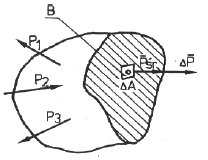
\includegraphics[width=5cm]{Zdjecia/2/potato}
\caption{Ciało pod wpływem sił zewnętrznych \cite{bartek_wolny}}
\label{fig:potato}
\end{figure}

Stana naprężenia w punkcie B oznacza ogół naprężeń, które otrzymamy dla wszystkich możliwych przekrojów ciała przez ten punkt.
W przypadku trójwymiarowego stanu naprężenia, dla każdego przekroju wektor naprężenia będzie miał inny kierunek. Stan naprężenia można opisać przy pomocy tensora naprężeń, dla układu kartezjańskiego danego wzorem:


\begin{gather}
	\sigma=\begin{bmatrix} 
	  \sigma_{xx}    & \tau_{xy} & \tau_{xz} \\ 
	  \tau_{yx} & \sigma_{yy} & \tau_{yz} \\
	  \tau_{zx} & \tau_{zy} & \sigma_{zz} 
	\end{bmatrix}
\end{gather}

gdzie

\begin{eqwhere}[2cm]
        \item[$\sigma_{ii}$] naprężenie normalne, i=(x, y, z)
        \item[$\tau_{ij}$] naprężenie styczne, i,j=(x, y, z), \( i \neq j, \tau_{ij}=\tau_{ji}\)
\end{eqwhere}

\subsection{Odkształcenie i prawko Hooke'a}
\label{sec:odksztalcenie_i_prawo_hookea}

	Pod wpływem naprężeń ciało sprężyste ulega odkształceniu. Możemy wyróżnić odkształcenia liniowe \( \varepsilon_i \) oraz odkształcenia postaciowe \( \gamma_{ij} \). Najprostszym przypadkiem odkształcenia liniowego jest rozciąganie pręta. Poniżej znajduje się rysunek pręta rozciąganego siłą P. 

\begin{figure}[h]
\centering
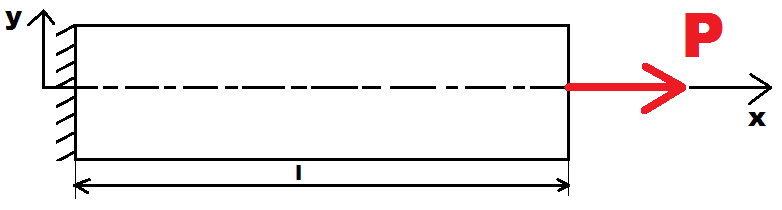
\includegraphics[width=10cm]{Zdjecia/2/rozciaganie}
\caption{Rozciąganie pręta}
\label{fig:rozciaganie}
\end{figure}

	W takim przypadku odkształceniem wzdłużnym będziemy nazywać stosunek wydłużenia pręta do jego początkowej długości:

\begin{equation}
\varepsilon_x=\frac{\Delta l}{l}.
\end{equation}
	
	Odkształceniem poprzecznym(postaciowym) nazywać będziemy stosunek zmiany średnicy przekroju do jego początkowej średnicy:

\begin{equation}
\varepsilon_y=\frac{\Delta d}{d}.
\end{equation}

	Odkształcenia te związane są zależnością:

\begin{equation}
\varepsilon_x=-\nu \varepsilon_y
\end{equation}
gdzie
\begin{eqwhere}[2cm]
        \item[$\nu$] współczynnik Poissona.
\end{eqwhere}

	Współczynnik Poissona jest wielkością bezwymiarową. Określa on sposób w jaki odkształca się ciało i przyjmuje wartości z przedziału [-1, 1]. Dla popularnych w mechanice stopów metali przyjmuje zwykle wartości z przedziału [0.2 , 0.4]. Wartości ujemne przyjmuje dla tak zwanych materiałów odwrotnych, które pod wpływem naprężenia zwiększają swoją objętość.

	Dla przypadku prostego rozciągania zachodzi jeszcze jedna zależność. Opisuje ona związek pomiędzy naprężeniem i odkształceniem i nazywana jest prawem Hooke'a.

\begin{equation}
\sigma=E\varepsilon
\end{equation}
gdzie
\begin{eqwhere}[2cm]
        \item[$E$] moduł Younga.
\end{eqwhere}

	Moduł Younga określa zależność odkształcenia liniowego i przyłożonego naprężenia. Jednostką moduły Younga jest paskal, a wartości podaje się w gigapasklach (GPa). Wartości dla stali wynoszą około 200 GPa, a dla aluminium około 70 GPa.

	W przypadku trójwymiarowego rozkładu okształceń stosuje się zapis tensorowy. Tensor odkształcenia znajduje się poniżej:
\begin{gather}
	\varepsilon=\begin{bmatrix} 
	  \varepsilon_{xx}    & \gamma_{xy} & \gamma_{xz} \\ 
	  \gamma_{yx} & \varepsilon_{yy} & \gamma_{yz} \\
	  \gamma_{zx} & \gamma_{zy} & \varepsilon_{zz} 
	\end{bmatrix}
\end{gather}

%\[
%	\textbf{$\varepsilon$}=\begin{bmatrix} 
%	  \varepsilon_{xx}    & \gamma_{xy} & \gamma_{xz} \\ 
%	  \gamma_{yx} & \varepsilon_{yy} & \gamma_{yz} \\
%	  \gamma_{zx} & \gamma_{zy} & \varepsilon_{zz} 
%	\end{bmatrix}
%\]

gdzie

\begin{eqwhere}[2cm]
        \item[$\varepsilon_{ii}$] odkształcenie liniowe, i=(x, y, z)
        \item[$\gamma_{ij}$] odkształcenie postaciowe, i,j=(x, y, z), \( i \neq j, \tau_{ij}=\tau_{ji}\)
\end{eqwhere}

Dla takiego przypadku prawo Hooke'a przybiera bardziej skomplikowaną postać:

\begin{equation}
\varepsilon_xx=\frac{1}{E}(\sigma_xx-\nu(\sigma_yy+\sigma_zz)), \gamma_{xy}=\frac{\tau_{xy}}{G}
\end{equation}
\begin{equation}
\varepsilon_yy=\frac{1}{E}(\sigma_yy-\nu(\sigma_xx+\sigma_zz)), \gamma_{xz}=\frac{\tau_{xz}}{G}
\end{equation}
\begin{equation}
\varepsilon_zz=\frac{1}{E}(\sigma_zz-\nu(\sigma_xx+\sigma_yy)), \gamma_{yz}=\frac{\tau_{yz}}{G}
\end{equation}

\begin{eqwhere}[2cm]
        \item[$G$] moduł Kirchoffa
\end{eqwhere}

	Moduł Kirchoffa opisuje zależność odkształcenia postaciowego od naprężenia stycznego występującego w materiale. Jednostką tego współczynnika jest paskal, a typowymi wartościami są dla stali 80 Gpa, dla aluminium 25,5 GPa.

	Opisane wcześniej stałe materiałowe są powiązane równaniem:
\begin{equation}
E=2G(\nu+1)
\end{equation}

%\begin{equation}
%c_L=\sqrt{\frac{\lambda+2\mu}{\rho}}
%\end{equation}
%gdzie
%\begin{eqwhere}[2cm]
%        \item[$c_L$] prędkość fali podłużnej
%        \item[$\lambda, \mu$] stałe Lam\'{e}go
%        \item[$\rho$] gęstość ośrodka
%\end{eqwhere}
%
%\begin{figure}[h]
%\centering
%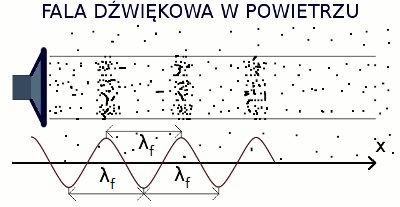
\includegraphics[width=10cm]{Zdjecia/2/fala_podluzna}
%\caption{Przykład fali podłużnej}
%\label{fig:fala_podluzna}
%\end{figure}
%
%
%
%\begin{figure}[h]
%        \centering
%        \begin{subfigure}{0.35\textwidth}
%                \centering
%	     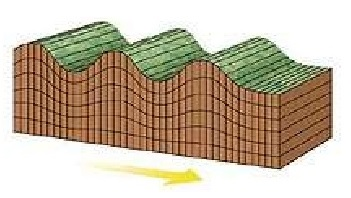
\includegraphics[width=5cm]{Zdjecia/2/fala_rayleigha}
%                \subcaption{\label{subfigure_a}}
%        \end{subfigure}
%        \begin{subfigure}{0.35\textwidth}
%                \centering
%	     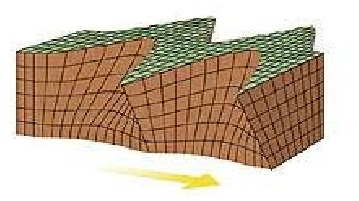
\includegraphics[width=5cm]{Zdjecia/2/fala_lova}
%                \subcaption{\label{subfigure_b}}
%        \end{subfigure}
%        \label{fig:subcaption_example}
%        \caption{Fale powierzchniowe: \protect\subref{subfigure_a} fala Rayleigha, \protect\subref{subfigure_b} fala L\"{o}va}
%\end{figure}

























\section{Rodzaje fal sprężystych}
\label{sec:rodzaje_fal_sprezystych}

Fale można podzielić ze względu na sposób w jaki propagują w materiale. Mogą to być fale podłużne lub poprzeczne. Fale takie propagują jeśli długość fali jest mniejsza lub bliska wymiarom ośrodka. Fale o długości przekraczającej wyraźnie przynajmniej jeden z wymiarów falowodu nazywamy falami prowadzonymi i mają one zupełnie inne własności. Do takich fal możemy zaliczyć np. fale Lamba. Fala Rayleigha z kolei propagują na powierzchniach, stąd ośrodek musi być ograniczony przynajmniej jedną płaszczyzną.

\subsection{Fale podłużne}

Fale podłużne to fale, w których kierunek propagacji jest równoległy z kierunkiem drgania cząstek. Tego typu fale mogą rozchodzić się w każdym ośrodku materialnym. Przykładem fali podłużnej jest fala dźwiękowa rozchodząca się w powietrzu, pokazana na Rys.2.1. Prędkoś fali podłużnej w nieograniczonym ośrodku zależy od parametrów materiałowych ośrodka i dana jest wzorem:

\begin{equation}
c_L=\sqrt{\frac{\lambda+2\mu}{\rho}}
\end{equation}
gdzie
\begin{eqwhere}[2cm]
        \item[$c_L$] prędkość fali podłużnej
        \item[$\lambda, \mu$] stałe Lam\'{e}go
        \item[$\rho$] gęstość ośrodka
\end{eqwhere}

\begin{figure}[h]
\centering
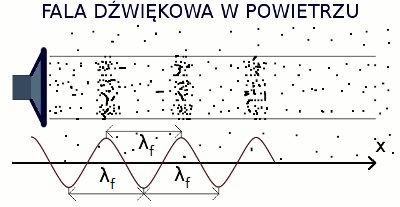
\includegraphics[width=10cm]{Zdjecia/2/fala_podluzna}
\caption{Przykład fali podłużnej}
\label{fig:fala_podluzna}
\end{figure}

Długością fali \( \lambda_f \) nazywamy odległoś między dwoma maksimami (lub minimami), które oznaczają maksymalne zagęszczenie (rozrzedzenie) cząstek w materiale.

\subsection{Fale poprzeczne}

Fale poprzeczne propagują w kierunku prostopadłum do kierunku drgań cząstek. Przykładami takich fal są fale elektromagnetyczne, fale propagacji naprężeń w materiale stałym, czy fala na zamocowanym jednostronnie sznurze, pokazana na Rys.2.2. Prędkoś fali poprzecznej w nieograniczonym ośrodku wyraża się wzorem:

\begin{equation}
c_T=\sqrt{\frac{\mu}{\rho}}
\end{equation}
gdzie
\begin{eqwhere}[2cm]
        \item[$c_T$] prędkość fali poprzecznej
        \item[$\mu$] stała Lam\'{e}go
        \item[$\rho$] gęstość ośrodka
\end{eqwhere}

\begin{figure}[h]
\centering
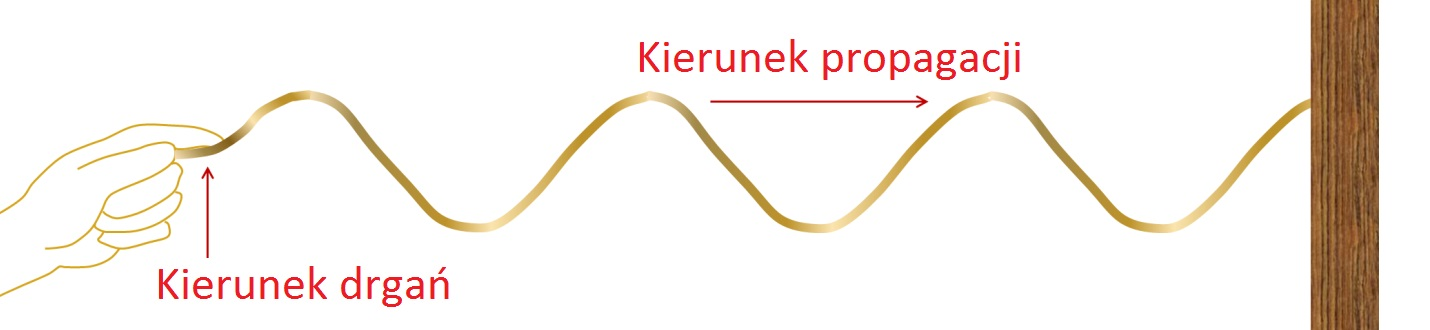
\includegraphics[width=10cm]{Zdjecia/2/fala_poprzeczna}
\caption{Przykład fali poprzecznej}
\label{fig:fala_poprzeczna}
\end{figure}

\subsection{Fale Rayleigha i L\"{o}va}

Opisane wcześniej fale propagują w nieograniczonych mediach. Fale Rayleigha oraz L\"{o}va są falami propagującymi w obszarze powierzchni ciał stałych. Dla fal Rayleigha drgania cząstek odbywają się równolegle oraz prostopadle do kierunku rozchodzenia się fali, zataczając elipsy. Kierunek prostopadły jest normalny do płaszczyzny, na której fala propaguje. Prędkoś fal Rayleigha dla metalu można wyrazić za pomocą współczynnik Poissona i prędkości fal poprzecznych:

\begin{equation}
c_R=\frac{0.87+1.12\cdot\nu}{1+\nu}\cdot c_T
\end{equation}
gdzie
\begin{eqwhere}[2cm]
        \item[$c_R$] prędkość fali Rayleigha
        \item[$c_T$] prędkość fali poprzecznej
        \item[$\nu$] współczynnik Poissona
\end{eqwhere}

Fale L\"{o}va to fale, w których drgania zachodzą w kierunku prostopadłym do kierunku, ale równolegle do płaszczyzny propagacji. Takie fale są wykorzystywane przy badaniu układów wielowarstwowych. Są silnie dyspersyjne, co oznacza że ich prędkość jest funkcją częstotliwości.

\begin{figure}[h]
        \centering
        \begin{subfigure}{0.35\textwidth}
                \centering
	     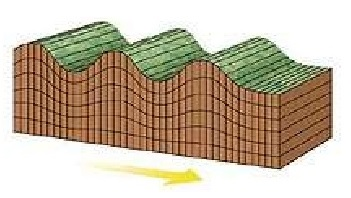
\includegraphics[width=5cm]{Zdjecia/2/fala_rayleigha}
                \subcaption{\label{subfigure_a}}
        \end{subfigure}
        \begin{subfigure}{0.35\textwidth}
                \centering
	     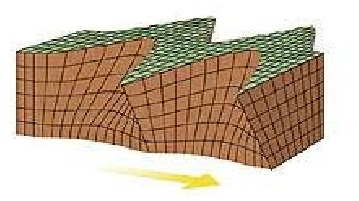
\includegraphics[width=5cm]{Zdjecia/2/fala_lova}
                \subcaption{\label{subfigure_b}}
        \end{subfigure}
        \label{fig:subcaption_example}
        \caption{Fale powierzchniowe: \protect\subref{subfigure_a} fala Rayleigha, \protect\subref{subfigure_b} fala L\"{o}va}
\end{figure}

\subsection{Fale Lamba}

Ważnym typem fal, z racji na szerokie zastosowanie, są fale Lamba. Propagują one na cienkościennych elementach jak płyty, czy rury. Tego typu fale powstają na skutek złożenia dwóch fal Rayleigha, propagujących na płaszczyznach po obu stronach obiektu. Fale Lamba można podzielić na fale symetryczne, kiedy obie fale składowe propagują w tej samej fazie i asntysymetryczne kiedy propagują w innych fazach. Prędkość fal Lamba zależna jest od częstotliwości, ze względu na dyspersyjny charakter.

\begin{figure}[h]
\centering
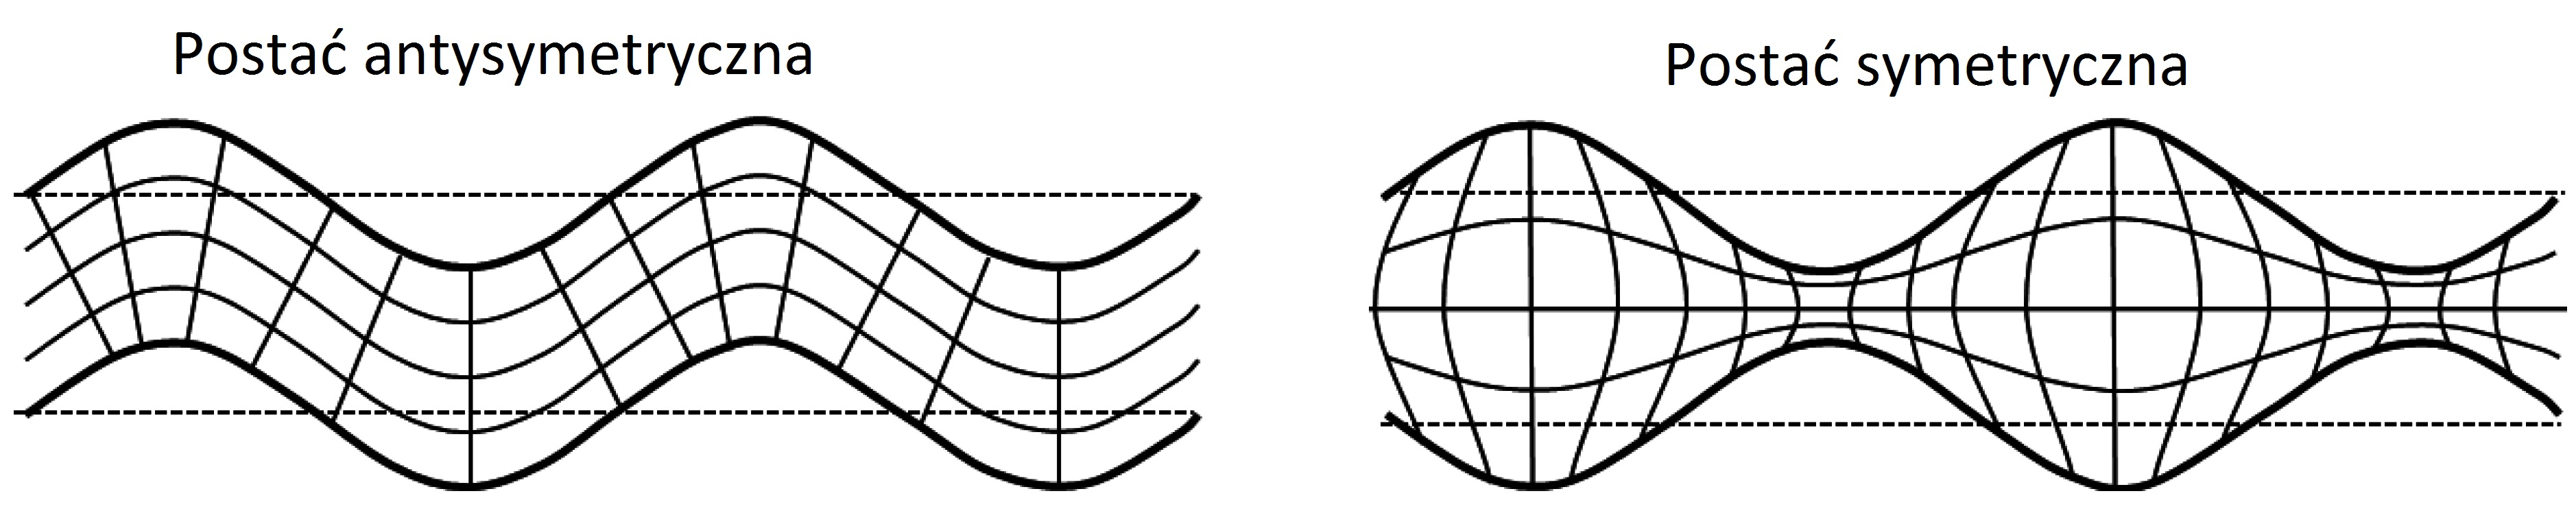
\includegraphics[width=14cm]{Zdjecia/2/fala_lamba}
\caption{Fale Lamba}
\label{fig:fala_lamba}
\end{figure}

%---------------------------------------------------------------------------
























\section{Zjawisko dyspersji}
\label{sec:rodzaje_fal_sprezystych}

Dyspersja jest zjawiskiem zależności prędkości propagacji fali od jej częstotliwości. Częstotliwością fali nazywamy liczbę pełnych przebiegów (np. od maximum do maximum) w jednostce czasu. Jednostką częstotliwości jest herc (Hz). Wielkością równie często używaną jest częstość kołowa dana wzorem \( \omega = 2\pi f \). Jej jednostką jest radian na sekundę [rad/s]. Odpowiednikiem tego parametru dla wymiarów geometrycznych jest liczba falowa. Określa ona jak wiele długości fali zawiera fala w jednostce odległości. Jednostką liczby falowej jest radian na metr [rad/m].

\begin{figure}[h]
\centering
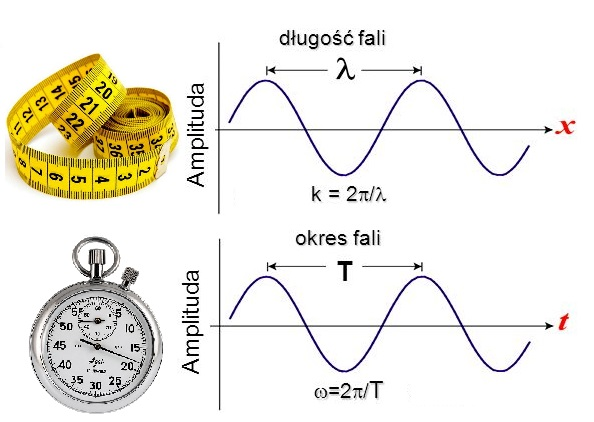
\includegraphics[width=10cm]{Zdjecia/2/czestotliwosc1}
\caption{Częstotliwość \( \omega \) i liczba falowa k}
\label{fig:czestotliwosc_i_liczba_falowa}
\end{figure}


Kiedy mówimy o krzywych dyspersji, możemy mieć na myśli zależności liczby falowej od częstotliwości, prędkości fazowej od częstotliwości lub prędkości grupowej od częstotliwości. Na rysunku \ref{fig:krzywe_k_od_omega} znajdują się przykładowe charakterystyki k(\(\omega\)) postaci fal Lamba dla aluminiowej płyty o grubości 1mm.

\begin{figure}[h]
\centering
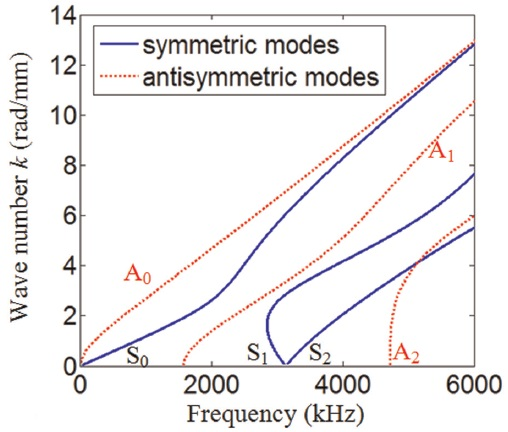
\includegraphics[width=10cm]{Zdjecia/2/char_fazowa}
\caption{Krzywe k(\(\omega\)) \cite{bartek_tian}}
\label{fig:krzywe_k_od_omega}
\end{figure}

Na wykresach widać jedną rzecz, ważną dla zastosowań fal prowadzonych - są one multimodalne. Z wykresów wynika, że w najkorzystniejszym do analizy przypadku propagują dwa mody, jeden symetryczny i jeden antysymetryczny. Wraz ze wzrostem częstotliwości propagującej fali pojawiają się dodatkowe jej postaci, co znacznie utrudnia analizę danych z przebiegów. Jednym ze sposobów ograniczania liczby modów, jest wprowadzanie wymuszeń o niskich częstotliwościach.

\subsection{Prędkość fazowa i grupowa}

Prędkość fazowa określa jak szybko przemieszcza się punkt fali o stałej fazie. Dla fali sinusoidalnej u(x,t)=sin(kx-\(\omega\)t) można wyznaczyć zależność na prędkość fazową w następujący sposób:

\begin{equation}
kx-\omega t=const \Rightarrow \frac{d(kx-\omega t)}{dt}=0 \Rightarrow k\frac{dx}{dt}-\omega=0
 \Rightarrow \frac{dx}{dt}=\frac{\omega}{k}
\end{equation}

Jak widać dla skończonej wartości \(\omega\) i k dążącego do zera, prędkość fazowa rośnie do nieskończoności. Dla przypadku pierwszych modów, gdzie zarówno k jak i \(\omega\) zmierzają do zera, sytuacja wygląda różnie. Na rysunku \ref{fig:krzywe_vp_od_omega} znajduje się przykładowy wykres zależności prędkości fazowej od iloczynu częstotliwości i grubości materiału dla cienkościennej rury. W przypadku fal prowadzonych dla elementów cienkościennych, często wykreśla się charakterystyki z zaznaczeniem wpływu grubości ściany. Na wykresie widać, że wszystkie mody poza pierwszymi dwoma dążą prawostronnie do nieskończoności. Pozostałe dwa zachowują się odmiennie - jeden wykres dąży do 0 (postać antysymetryczna), a drugi do wartości skończonej (postać symetryczna).

\begin{figure}[h]
\centering
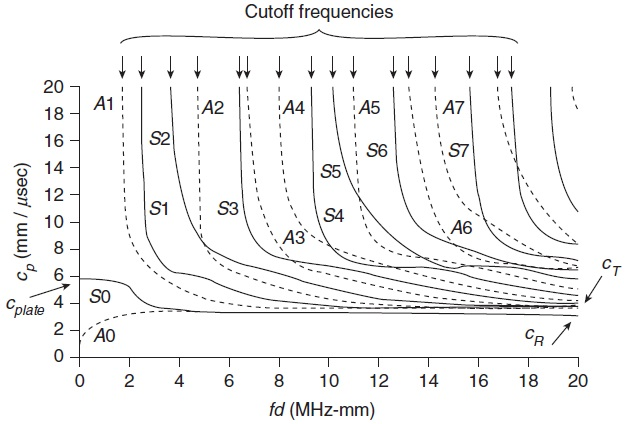
\includegraphics[width=10cm]{Zdjecia/2/char_predkosc_fazowa}
\caption{Krzywe \(V_p(\omega\)) \cite{bartek_rose}}
\label{fig:krzywe_vp_od_omega}
\end{figure}

Jeśli fala składa się z więcej niż jednej składowej sinusoidalnej, które mają różne prędkości, należy określić jeszcze prędkość grupową.  Prędkość każdej z pojedynczych składowych, będzie jej prędkością fazową. Prędkość grupowa dotyczy sygnału, złożonego ze wszystkich składowych. Można ją prezentować jako prędkość punktu o zmiennej fazie na wykresie sygnału, np. maximum, jak na rysunku \ref{fig:przykladowy_sygnal}.

\begin{figure}[h]
\centering
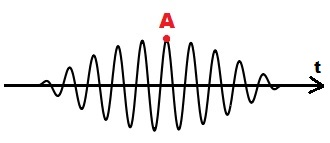
\includegraphics[width=10cm]{Zdjecia/2/predkosc_grupowa_wierzcholek}
\caption{Przykładowy sygnał. Prędkość punktu A jest prędkością grupową}
\label{fig:przykladowy_sygnal}
\end{figure}

Weźmy sygnał złożony z kilku sinusoid o zbliżonej częstości. Fazę każdego sygnału można zapisać jako \( \omega_i t - k_i T + \phi_i \), gdzie \( i\) oznacza numer składowej. Założmy, że fazy tych sygnałów są równe w punkcie x=0, t=0. Wynika stąd, że \( \phi_i \) są niezależne od \( \omega \). Punkt x=0, t=0 będzie maksimum, ponieważ wszystkie składowe zsumują się w tym punkcie. Aby znaleźć kolejny punkt z takim maximum, należy określić gdzie fazy po raz kolejny będą sobie równe.  Punkt, w którym to zjawisko zajdzie musi być niezależny od \( \omega \), w otoczeniu pewnego \( \omega \). Symbolicznie można to zapisać jako:

\begin{equation}
\frac{d(\omega t - kx - \phi)}{d\omega}=0 \Rightarrow t-\frac{dk}{d\omega}x=0 \Rightarrow \frac{x}{t}=\frac{d\omega}{dk}
\end{equation}

Maximum sygnału będzie więc w każdym punkcie x, t spełniającym powyższą zależność. Prędkość grupowa fali jest więc równa:

\begin{equation}
V_g=\frac{dw}{dk}
\end{equation}

Z samego faktu istnienia takiej zależności nie wynika, że w sygnale znajdzie się jakiś charakterystyczny punkt, propagujący z taką prędkością. Wynika z niej natomiast, że jeśli takowy punkt będzie, to będzie się poruszał z prędkością grupową. Należy jeszcze wspomnieć o wyznaczaniu prędkości grupowej sygnału o składowch, o różnych wartościach \( \omega \). W takim przypadku należy prędkość grupową wyznaczyć dla wartości \(\omega\) sygnału dominującego. Dominujący sygnał można znaleźć przy pomocy przekształecenia Fouriera.

Na rysunku \ref{fig:predkosc_grupow_wykres} znajdują się przykładowe krzywe, przedstawiające prędkość grupową dla fal Lamba, dla cienkościennej płyty aluminiowej.

\begin{figure}[h]
\centering
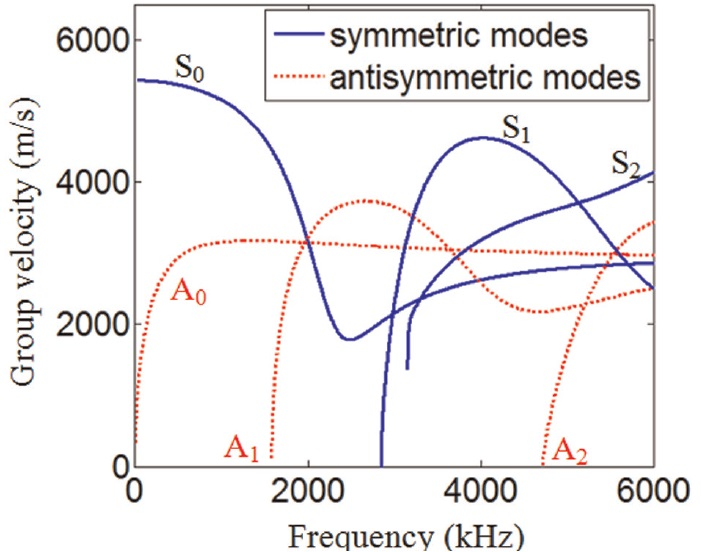
\includegraphics[width=10cm]{Zdjecia/2/predkosc_grupowa_wykres}
\caption{Wykres prędkości grupowej \(V_g(\omega)\) \cite{bartek_tian}}
\label{fig:predkosc_grupow_wykres}
\end{figure}


\subsection{Analityczne wyznaczanie krzywych dyspersji}

Zależności dyspersyjne są trudne, a często niemożliwe do wyznaczenia w sposób analityczny. Dla prostych przypadków rozwiązania analityczne są znane, a kilka z nich jest poniżej opisanych w celu lepszego wyjaśnienia zjawiska dyspersji.
Pierwszym przypadkiem będzie model nieskończenie długiej, napiętej sprężyny, przedstawionej na rysunku \ref{fig:nieskonczenie_krotki_odcinek_sprezyny}.

\begin{figure}[h]
\centering
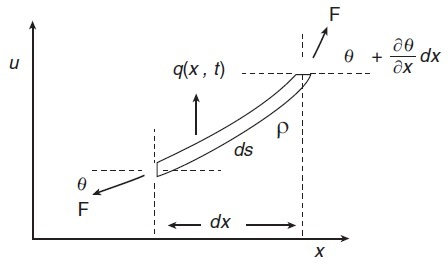
\includegraphics[width=10cm]{Zdjecia/2/dyspersja_analitycznie_sprezyna}
\caption{Nieskończenie krótki odcinek napiętej sprężyny \cite{bartek_rose}}
\label{fig:nieskonczenie_krotki_odcinek_sprezyny}
\end{figure}

Symbole z rysunku oznaczają:

\begin{eqwhere}[2cm]
        \item[$ds$] długość sprężyny
        \item[$\theta$] kąt przyłożenia siły zewnętrznej
        \item[$F$] siły wewnętrzne
        \item[$q$] siła oddziaływania sprężyny na jednostkę długości ugięcia
        \item[$\rho$] masa sprężyny na jednostkę długości.
\end{eqwhere}

Korzystając z drugiej zasady dynamiki Newtona, zapisujemy równanie ruchu układu:

\begin{equation}
-Fsin\theta+Fsin(\theta+\frac{\partial \theta}{\partial x}dx)+qds = \rho ds \frac{\partial^2u}{\partial t^2}.
\end{equation}

Załóżmy dodatkowo, że:

\begin{equation}
ds \approx dx\; ,\; sin\theta=\theta \; i\; \theta = \frac{\partial u}{\partial x}.
\end{equation}

To pozwala uprościć równanie:

\begin{equation}
-F\theta+F(\theta + \frac{\partial \theta}{\partial x}dx)=\rho dx\frac{\partial^2 u}{\partial^2 t}
\end{equation}

\begin{equation}
F\frac{\partial^2 u}{\partial x^2} + q = \rho \frac{\partial^2 u}{\partial^2 t}.
\end{equation}

Jeśli założymy brak siły zewnętrznej, to otrzymujemy proste równanie falowe:

\begin{equation}
\frac{\partial^2 u}{\partial x^2} = \frac{1}{c_0^2} \frac{\partial^2 u}{\partial^2 t},\quad c_0=\sqrt{\frac{F}{\rho}}
\end{equation}

gdzie
\begin{eqwhere}[2cm]
        \item[$c_0$] prędkość fali.
\end{eqwhere}

Przyjmijmy rozwiązanie w postaci:

\begin{equation}
u(x,t)=Ae^{i(kx-\omega t)}.
\end{equation}

Jeśli wstawimy je do równania falowego to otrzymamy zależność dyspersyjną:

\begin{equation}
\omega^2=c_0^2 k^2.
\end{equation}

Jest to przypadek liniowej zależności \( k(\omega)\), a więc dyspersja fali nie zachodzi. W takim przypadku prędkość fazowa, jest równa prędkości grupowej:

\begin{equation}
V_p=\frac{\omega}{k}=\frac{d\omega}{dk}=V_g
\end{equation}

Prosta modyfikacja układu ze sprężyną jak na rysunku \ref{fig:nieskonczenie_krotki_odcinek_sprezyny2}, powoduje skomplikowanie zależności dyspersyjnej.

\begin{figure}[h]
\centering
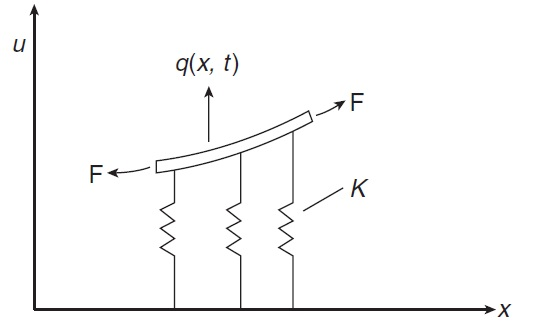
\includegraphics[width=10cm]{Zdjecia/2/dyspersja_analitycznie_sprezyna2}
\caption{Nieskończenie krótki odcinek napiętej sprężyny na sprężystym podłożu \cite{bartek_rose}}
\label{fig:nieskonczenie_krotki_odcinek_sprezyny2}
\end{figure}

Przyjmijmy siłę \(q=-Ku(x,t)\), co prowadzi do równania równowagi:

\begin{equation}
\frac{\partial^2 u}{\partial x^2} - \frac{K}{F}u = \frac{1}{c_0^2} \frac{\partial^2 u}{\partial^2 t}.
\end{equation}

Ponownie załóżmy rozwiązanie w postaci \( u(x,t)=Ae^{i(kx-\omega t)} \) i podstawmy je do równania równowagi. Prowadzi to do zależności:

\begin{equation}
\Big(-k^2-\frac{K}{F}+\frac{w^2}{c_0^2}\Big)e^{i(kx-\omega t)}=0.
\end{equation}

Równanie to jest nazywane równaniem charaktersytycznym (lub dyspersyjnym). Rozwiązaniem jest:

\begin{equation}
-k^2-\frac{K}{F}+\frac{w^2}{c_0^2}=0.
\end{equation}

Zależność \(k(\omega)\) przyjmuje postać:

\begin{equation}
k^2=\frac{w^2}{c_0^2}-\frac{K}{F}.
\end{equation}

Podstawiając \( k=\frac{\omega}{c_p}\), otrzymujemy :

\begin{equation}
c_p = \sqrt{c_0^2\Bigg( \frac{1}{1 - \frac{c_0^2 K}{\omega^2 F} } \Bigg)}.
\end{equation}

Jak widać w takim przypadku prędkość fazowa jest zależna od częstotliwości, a więc będzie zachodzić dyspersja fali.

\vspace{3mm}

Kolejnym problemem wartym wspomnienia, jest problem propagacji fal Lamba w cienkiej, nieskończonej płycie. Płyta wraz z przyjętym układem współrzędnych znajduje się na rysunku \ref{fig:nieskonczona_plyta}.

\begin{figure}[h]
\centering
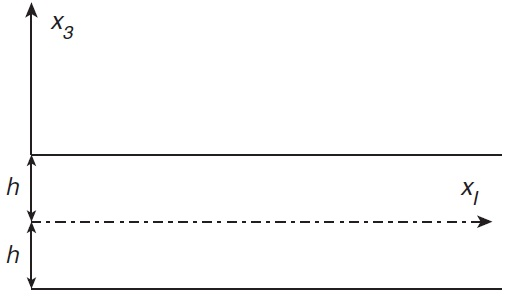
\includegraphics[width=10cm]{Zdjecia/2/dyspersja_analitycznie_plyta}
\caption{Nieskończona płyta \cite{bartek_rose}}
\label{fig:nieskonczona_plyta}
\end{figure}

Jest kilka metod rozwiązania takiego zagadnienia, ale nie są opisane one w tej pracy (metoda potencjałów, metoda fal cząstkowych). Jeśli przyjmiemy zerowe naprężenia na płaszczyznach zewnętrznych jako warunki początkowe, to związki dyspersyjne przyjmują zależności:

\begin{equation}\label{fig:RL1}
\frac{tan(qh)}{tan(ph)}=-\frac{4k^2pq}{(q^2-k^2)^2}
\end{equation}
dla postaci symetryczych oraz

\begin{equation}\label{fig:RL2}
\frac{tan(qh)}{tan(ph)}=-\frac{(q^2-k^2)^2}{4k^2pq}
\end{equation}
dla postaci antysymetrycznych,

gdzie
\begin{equation}
p^2=\frac{\omega^2}{c_L^2} - k^2 \; ,a \; q^2=\frac{\omega^2}{c_L^2}-k^2
\end{equation}

\begin{eqwhere}[2cm]
        \item[$c_T$] prędkość fali poprzecznej
	\item[$c_L$] prędkość fali podłużnej
\end{eqwhere}

Równania \ref{fig:RL1}, \ref{fig:RL2} nazywają się równaniami Rayleigha-Lamba i są nierozwiązywalne w sposób analityczny. Jest to przykład bardziej skomplikowanego modelu, gdzie możliwe jest wyznaczenie związków \(k\) i \(\omega\), ale do wykreślenia krzywych dyspersji konieczne jest zastosowanie metod numerycznych.



\subsection{Numeryczne wyznaczanie krzywych dyspresji}
Pierwszym przypadkiem numerycznego wyznaczania krzywych dyspersji, jest rozwiązanie równań Rayleigha-Lamba przedstawionych w poprzedniej sekcji. Zakładamy, że interesują nas tylko rozwiązania rzeczywiste, które pojawią się jeśli k przyjmie wartości rzeczywiste bądź urojone (w równaniach występuje tylko czynnik \(k^2\)).

Poniżej znajdują się równania Rayleigha-Lamba w postaci ułatwiającej proponowany sposób rozwiązania:

\begin{equation}
\frac{tan(qh)}{q}+\frac{4k^2ptan(ph)}{{q^2-k^2}^2}=0
\end{equation}

\begin{equation}
qtan(qh)+\frac{{(q^2-k^2)}^2tan(ph)}{2k^2p}=0.
\end{equation}

\vspace{5mm}

Rozwiązać równanie możemy według przedstawionego algorytmu.

\begin{enumerate}
  \item Wybierz iloczyn \((\omega h)_0\).
  \item Wybierz początkową estymatę prędkości fazowe \((c_p)_0\) (a pośrednio też \(k\)).
  \item Oblicz znak lewych stron równań R-L.
  \item Wybierz kolejną wartość prędkości fazowej \((c_p)_1 > (c_p)_0\) i policz znaki lewych stron jeszcze raz.
  \item Powtarzaj kroki 3 i 4 aż znaki się zmienią. Oznaczać to bedzie, że pierwiastek równania znajduje się pomiędzy ostatnio wybranymi prędkościami. Załóżmy, że jest to pomiędzy \( (c_p)_n \) i \( (c_p)_{n+1} \).
  \item Wykorzystaj jakiś algorytm iteraycjny do znalezienia pierwiastka \(c_p\) z odpowiednią dokładnością.
   \item Po znalezienu pierwiastka, kontynuuj wyszukiwnie kolejnych pierwiastków dla założonego \( (\omega h)_0 \), powtarzając kroki 2-6.
  \item Wybierz kolejną wartość \( \omega h \) i wykonaj dla niej kroki 2-7.
\end{enumerate}

\vspace{5mm}

W ten sposób łatwo wyznaczyć krzywe dyspersji, ale należy zaznaczyć, że równania dyspersyjne zostały obliczone analitycznie dla konkretnego przypadku struktury, jaką jest płyta. Metody numeryczne ograniczają się w tym przypadku do rozwiązania wyznaczonych równań. Możliwość ogólniejszego podejścia do badań numerycznych, dla szerokiego wachlarza struktur daje metoda elementów skończonych.

Metoda ta daje możliwości dokładnego przewidzenia odpowiedzi dynamicznych, dla złożonych układów mechanicznych. Jeśli założymy przypadek małych odkształceń, to problem można zapisać w postaci równania różniczkowego:

\begin{equation} \label{eq:MES1}
M\ddot u + Ku = f^{ext}
\end{equation}

gdzie
\begin{eqwhere}[2cm]
        \item[$M$] macierz mas układu
        \item[$K$] macierz sztywności układu 
        \item[$u$] przemieszczenia punktów układu
        \item[$f^{ext}$] wektor sił zewnętrznych
\end{eqwhere}

Sposobem wyznaczenia krzywych dyspersji z tak określonego układu, może być rozwiązanie równania tj. znalezienie pola przemieszczeń dla wszystkich węzłów w dyskretnych chwilach czasowych, a następnie obliczenie wielowymiarowego przekształcenia Fouriera otrzymanego sygnału.

Równanie można rozwiązać na przykład z wykorzystaniem centralnej formuły różnicowej dla \( \ddot u\):

\begin{equation}
\ddot x = \frac{u^{t+1} - 2u^t + u^{t-1}}{\Delta t^2}.
\end{equation}

Po podstawienu otrzymujemy zależność:

\begin{equation}
\frac{1}{\Delta t^2}M(u^{t-1}-2u^t+u^{t-1}) + Ku^t = f^t
\end{equation}

\begin{equation}
u^{t+1}=\Delta t^2 M^{-1}(f^t -Ku^t)+2u^t-u^{t-1}
\end{equation}

gdzie \( t \) oznacza obecną chwilę czasową, a \( t+1 \) chwilę kolejną.
Operacja odwracania macierzy mas jest kosztowna obliczeniowo. Można przyśpieszyć obliczenia przez zastosowanie skupionej macierzy mas (wyrazy niezerowe tylko na głownej diagonali).

Jeśli interesuje nas propagacja tylko w jednym kierunku, to dla obliczonego sygnału \( u[m, n] \) (m - liczba kroków czasowych \(\Delta t \) , n - liczba kroków geometrycznych \(\Delta x\) w kierunku x) przekształcenie Fouriera można obliczyć według wzoru:

\begin{equation} \label{eq:fourier_2d}
U[p, q] = \sum_{k=0}^{m-1} \sum_{l=0}^{n-1} u[k, l]e^{-i2\pi (-p \frac{k}{m} + q\frac{l}{n})}
\end{equation}

Mając dyskretną postać przekształcenia Fouriera można wykreślić krzywe dyspersji, wyznaczając dla każdej próbki wartość czętotliwości i liczby falowej. Można to zrobić wiedząc, że częstość zawiera się w przedziale \([0, \frac{1}{2\Delta t}2\pi]\), a liczba falowa \([0, \frac{1}{2\Delta x}2\pi]\). Przykładowe krzywe przedstawione są na rysunku \ref{fig:krzywe_dyspersji_tian1}.

\vspace{5mm}

\begin{figure}[h]
\centering
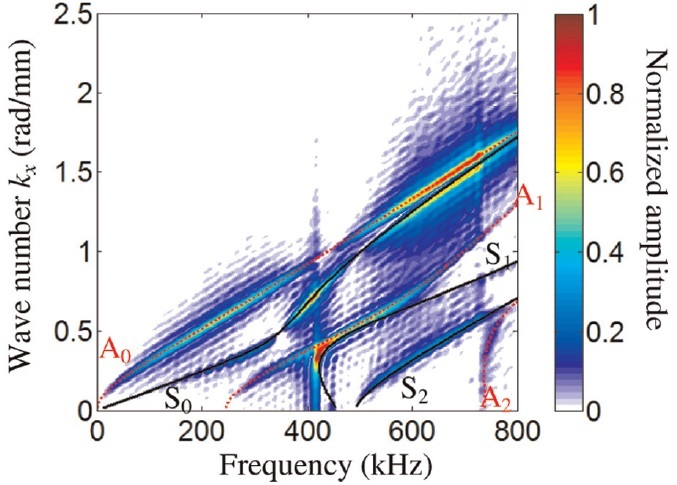
\includegraphics[width=10cm]{Zdjecia/2/dyspersja_tian1}
\caption{Krzywe dyspersji wyznaczone przy pomocy dwuwymiarowego DFT}
\label{fig:krzywe_dyspersji_tian1}
\end{figure}

Innym sposobem wyznaczania krzywych dyspersji z pomocą modelu MES, jest symulacja układu dla wymuszeń harmonicznych o ustalonych częstotliwościach, w których chcemu wyznaczyć krzywe. Jako przyład rozpatrzmy jednorodny pręt. Dla przypadku pręta wymuszanego na jednej płaszczyźnie przekroju, dane należy zebrać przed odbiciem fali od swobodnego końca pręta, tak aby sygnał propagował tylko w jednym kierunku. W liniach równoległych do osi, obliczamy pola prędkości przemieszczenia punktów. Może to być też pole przemieszczeń lub naprężeń, ale pole prędkości jest stosunkowo łatwe do wyznaczenia.
Znając już prędkości dla wszystkich punktów w jednej lini, w chwili t, możemy wyznaczyć widmo otrzymanego sygnału. Następnie z widma sygnału odczytujemy liczby falowe, dla których powstały widoczne piki. Pik dla największej liczby falowej dotyczy pierwszego modu, a każdy kolejny, z coraz mniejszymi liczbami falowymi, modów kolejnych.

Pole prędkości można wyznaczyć na podstawie różnycowych formuł centralnych \ref{eq:MES2} oraz \ref{eq:MES3}.

\begin{equation} \label{eq:MES2}
\dot u^{t+1} = \dot u^n + \frac{\Delta t}{2}(\ddot u^n + \ddot u^{n+1})
\end{equation}

\begin{equation} \label{eq:MES3}
u^{n+1} = u^n + \Delta t(\dot u^n + \frac{\Delta t}{2}\ddot u^n)
\end{equation}

Załóżmy, że znamy pełne rozwiązanie w chwili t. Przemieszczenie w chwili t+1 możemy więc obliczyć z zależności \ref{eq:MES3}. Następnie podstawiamy wynik do równania \ref{eq:MES1} i obliczamy przyspeszenie w chwili t+1. Ostatecznie korzystając z formuły \ref{eq:MES2} możemy wyznaczyć prędkość w chwili t+1.

Przykładowe widmo, z którego możemy odczytać liczby falowe czterech modów znajduje się na rysnuku \ref{fig:widmo_wymuszenie1}. Jak widać nie wszystkie liczby falowe da się wykryć przy pomocy danych z jednej lini, więc niezbędne jest prowadzenie obliczeń dla kilku różnych linii.

\begin{figure}[h]
\centering
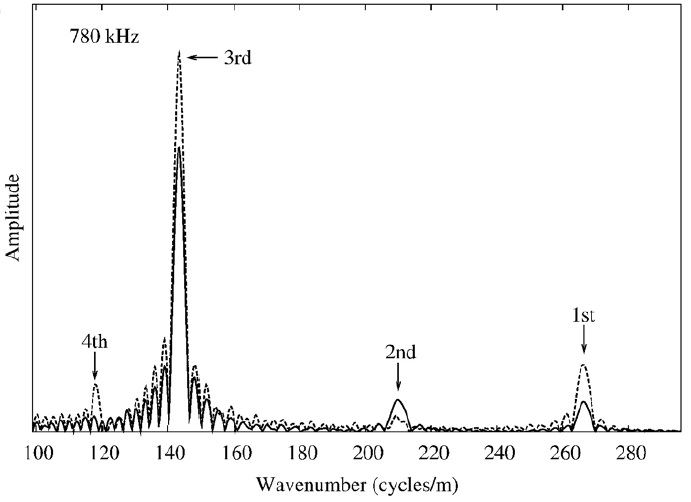
\includegraphics[width=10cm]{Zdjecia/2/widmo_wymuszenia_waskopasmowe}
\caption{Widmo sygnału prędkości na liniach równoległych do osi pręta}
\label{fig:widmo_wymuszenie1}
\end{figure}

Wadą tego sposobu jest konieczność prowadzenia obliczeń dla każdej częstotliwości, dla jakiej chcemy mieć punkty krzywych dyspersji. Jedne przebieg daję nam tylko jeden punkt na każdej krzywej. Fakt prowadzenia obliczeń tylko w liniach równoległych do osi pręta, ogranicza dodatkow obszar propagujących fal do fal podłużnych.

\vspace{3mm}

Sposobem zmniejszenia liczby symulacji jakie trzeba przeprowadzić jest symulacja z wymuszeniem szerokopasmowym. Pozwala to na uzyskanie informacji o krzywych dyspersji, dla częstotliwości zawierających się w wymuszającym sygnale. Pojawia się jednak kilka dodatkowych kroków jakie trzeba wykonać, aby uzyskać liczby falowe modów dla poszczególnych częstotliwości.

Aby uzyskać dane do wykreślenia krzywych dyspersji, należy obliczyć przestrzenny rozkład prędkości na liniach równoległych do osi dla wszystkich częstotliwości. W tym celu trzeba wykonać następujące czynności.

\begin{enumerate}
  \item Wyznaczyć odpowiedzi czasowe dla każdego punktu na interesującej nas lini równoległej do osi pręta.
  \item Obliczyć transformaty Fouriera tych sygnałów
  \item Z widma sygnału w każdym punkcie pobrać informacje o amplitudzie dla kolejnych częstotliwości. Na tej podstawie odtworzyć amplitudowy przebieg sygnału na całej lini dla każdej interesującej nas częstotliwości.
  \item Dla obliczonych w pkt. 3 przebiegów, obliczyć transformatę Fouriera i z wykresu odczytać wartości liczby falowej, dla wybranych częstotliwości.
\end{enumerate}

Rysunki \ref{fig:szer_odp_czasowe} oraz \ref{fig:szer_odp_przestrzenne} przedstawiają kolejne kroki postępowania, dla odpowiedzi na wymuszenie krokiem jednostkowym preta zbudowanego z 1601 węzłów na długości jednej lini. 

\begin{figure}[h]
\centering
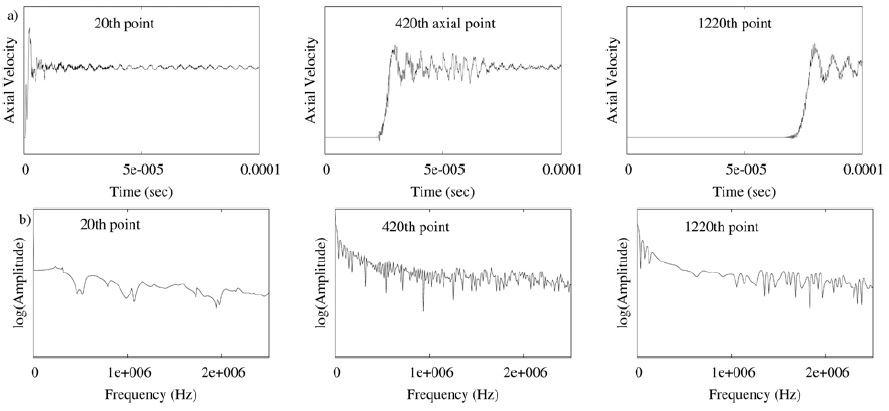
\includegraphics[width=12cm]{Zdjecia/2/widmo_wymuszenia_szerokopasmowe1}
\caption{a) Odpowiedzi na szerokopasmowe wymuszenie w wybranych punktach jednej lini b) Przekształcenia Fouriera odpowiedzi czasowych}
\label{fig:szer_odp_czasowe}
\end{figure}

\begin{figure}[h]
\centering
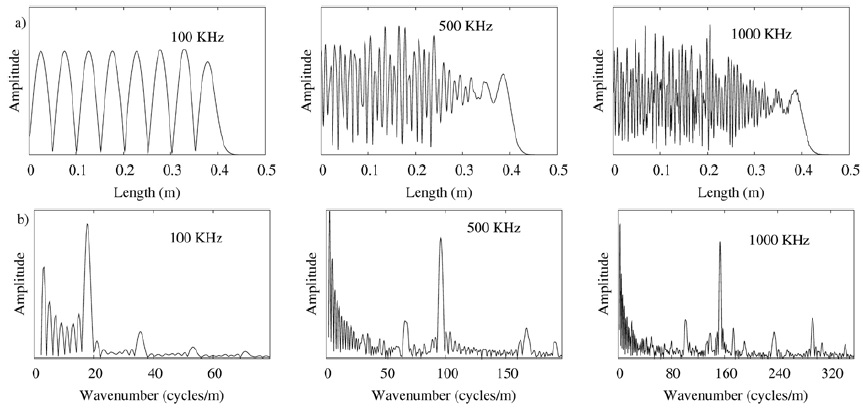
\includegraphics[width=12cm]{Zdjecia/2/widmo_wymuszenia_szerokopasmowe2}
\caption{a) Odtworzony sygnał apmlitudowy na długości pręta w jednej lini b) Przekształcenie Fouriera odtworzonych sygnałów}
\label{fig:szer_odp_przestrzenne}
\end{figure}

\vspace{3mm}

Ostatnia przedstawiona tutaj metoda skupia się, na rozwiązaniu zagadnienia własnego modelu wyznaczonego z pomocą MES. Tym razem zakładać będziemy wybraną liczbę falową i dla niej obliczać częstości poszczególnych modów. 
Po raz kolejny za przykład weźmy pręt. Pręt dzielimy na komórki, które będą się składać z kolejnych płaszczyzn, na których znajdują się węzły. Znając odległość płaszczyzn i wybierając liczbę falową, możemy okrelić przesunięcie fazowe fali pomiędzy płaszczyznami. Sytuacja przedstawiona jest na rysunku \ref{fig:komorki_preta}.


\begin{figure}[h]
\centering
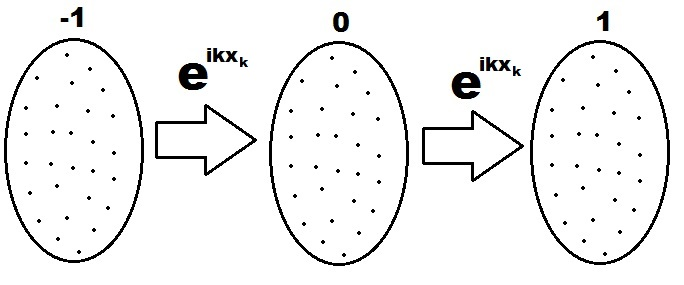
\includegraphics[width=10cm]{Zdjecia/2/metoda_numeryczna3}
\caption{Kolejne komórki pręta}
\label{fig:komorki_preta}
\end{figure}

W liniowych systemach do opisu popagacji fali wystarcza jedna komórka i siły wewnętrzne pochodzące od komórek sąsiednich. W przypadku braku sił zewnętrznych i przy założeniu skupionej macierzy mas, równanie układu można zapisać w postaci \ref{eq:MES4}. Rysunek \ref{fig:komorki_preta_sztywnosc} przedstawia sposób wyznaczania macierzy sztywności dla komórki środkowej, z uwzględnieniem zależności z komórkami sąsiednimi.

\begin{equation} \label{eq:MES4}
M_0\ddot x_0 + \sum_{p=-1}^1 K_p x_p = 0
\end{equation}

\begin{figure}[h]
\centering
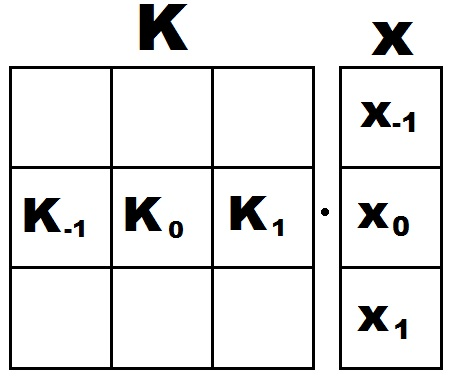
\includegraphics[width=8cm]{Zdjecia/2/metoda_numeryczna3_sztywnosc}
\caption{Wyznaczanie macierzy sztywności środkowej komórki z uwzględnieniem zależności z komórkami sąsiednimi}
\label{fig:komorki_preta_sztywnosc}
\end{figure}

Uwzględniając wszystkie informacje równanie układu można zapisać jako \ref{eq:MES5}. Podstawiając dodatkowo zależności \( \ddot x = x \omega^2 \), \( M_{sys} = M_0 \) oraz \( K_{sys} = K_{-1} e^{-ikx_k} + K_0 + K_1 e^{ikx_k} \) otrzymujemy równanie \ref{eq:MES6}.

\begin{equation} \label{eq:MES5}
M_0\ddot x_0 + K_{-1} x_0 e^{-ikx_k} + K_0 x_0 + K_1 x_0 e^{ikx_k} = 0
\end{equation}

\begin{equation} \label{eq:MES6}
 (M_{sys}\omega^2 + K_{sys})x_0 = 0
\end{equation}

Ostatecznie rozwiązując zagadnienie własne dla pary macierzy \( M_{sys} \) i \( K_{sys} \) otrzymujemy kwadraty częstości własnych układu dla założonego \( k \). Każda z częstości należy do jednego modu krzywych dyspersji.

Wadami tej metody są konieczność prowadzenia obliczeń dla każdej liczby falowej, którą chcemy uwzględnić w wynikach, oraz brak dokładnej informacji, która częstość własna należy do której postaci fali.

Dużą zaletą z kolei jest fakt, że wyznaczamy jedną metodą krzywe dyspersji dla fal podłużnych i poprzecznych.

Przykładowe krzywe dyspersji uzyskane w ten sposób przedstawia rysunek \ref{fig:przykladowe_krzywe}.

\begin{figure}[h]
\centering
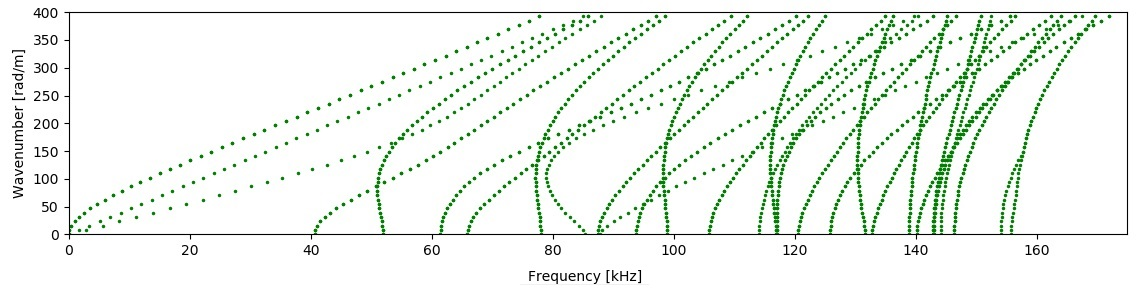
\includegraphics[width=14cm]{Zdjecia/2/przykladowe_krzywe}
\caption{Krzywe uzyskane przez wielokrotne rozwiązanie zagadnienia własnego pręta}
\label{fig:przykladowe_krzywe}
\end{figure}



\subsection{Eksperymentalne wyznaczanie krzywych dyspersji}

Eksperymentalne badania fal prowadzonych przeprowadza się wzbudzając odpowiednio obiekt, a następnie zbiera się dane o powstałej fali w innych punktach konstrukcji lub w tym samym punkcie po odbiciu fali. Zebrane dane analizuje się za pomocą algorytmów, w których duże znaczenie ma przekształcenie Fouriera.

Jako wzbudniki fal prowadzonych często stosowane są przetworniki piezoelektryczne (na przykład z ceramik PZT). Proste zjawisko piezoelektryczne z jakiego korzystają takie przetworniki, pozwala przekształcić energię elektryczną na energię mechaniczną. Efekt odwrotny pozwala zbierać informację o energi odkształcenia w materiale i sygnał mechaniczny przekształcić w elektryczny. 

Materiały piezoelektryczne znalazły szerokie zastosowanie ze względu na dobre parametry mechaniczne, odporność na wiele substancji chemicznych oraz bardzo duże możliwości kształtowania przetworników. Wzbudniki i sensory piezoelektryczne często występują jako cienkie fragmenty materiału piezoelektrycznego, które można wykonać w dowolnym kształcie. W przypadku kiedy chcemy uzyskać większą apmlitudę wzbudzenia, stosuje się stosy stworzone z wielu warstw piezoelektryka.

Obecna ilość dostępnych na rynku rozwiązań pozwala na dobranie odpowiedniego przetwornika do niemal każdego projektu bazującego na niskich częstotliwościach. Podczas analizy rozwiązań komercyjnych okazało się, że duża część takich przetowrników posiada ograniczenia działania do kilku kHz. Jest to najczęściej zbyt niska częstotliwość, nawet w przypadku badania wyłącznie modów podstawowych. Dostępne są też rozwiązania dla częstotliwości do nawet kilkuset kHz, co w przypadku fal prowadzonych może stanowić wystarczającą wartość.

Przykłady przetworników piezoelektrycznych w formie płytki oraz stosu znajdują się na rysunku \ref{fig:piezoelektryki}.

\begin{figure}[h]
        \centering
        \begin{subfigure}{0.35\textwidth}
                \centering
	     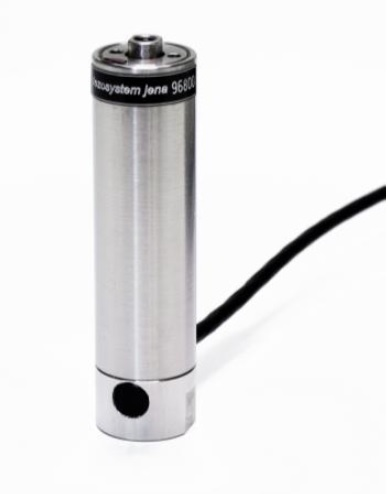
\includegraphics[width=5cm]{Zdjecia/2/piezo_stos}
                \subcaption{\label{subfigure_a}}
        \end{subfigure}
        \begin{subfigure}{0.35\textwidth}
                \centering
	     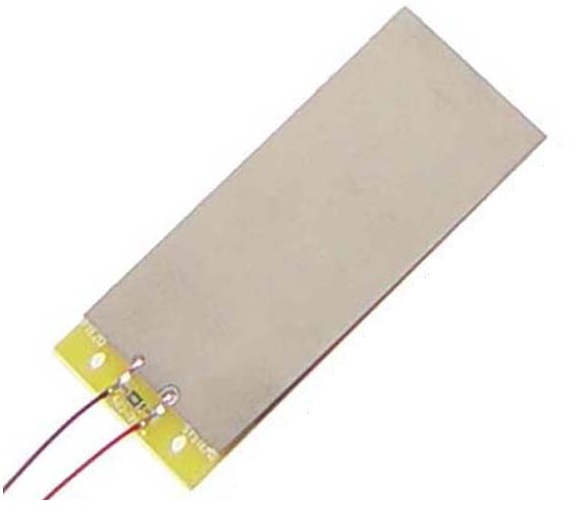
\includegraphics[width=5cm]{Zdjecia/2/piezo_plytka}
                \subcaption{\label{subfigure_b}}
        \end{subfigure}
        \caption{Przetworniki piezoelektryczne: \protect\subref{subfigure_a} w formie sotsu, \protect\subref{subfigure_b} w formie płytki}
        \label{fig:piezoelektryki}
\end{figure}

\vspace{3mm}

Innym sposobem badań jest wykorzystanie techniki laserowej. Za pomocą wiązki lasera możliwe jest wzbudzenie fal sprężystych w materiale. Na szczególną uwagę zasługuje możliwość wzbudzenia fali krótki impulsem, którego widmo będzie miało bardzo duży zakres częstotliwości. Sygnał taki możemy porównać do delty Diraca, dla której widmo ma stałą amplitudę. 

Za pomocą lasera możemy wykonywać także pomiary drgań materiału. Posłużyć może do tego na przykład interferometr laserowy, wykorzystujący efekt Dopplera. Detekcja jest jednak ograniczona do fal powierzchniowych. Atutem takiego pomiaru jest możliwość wykonania go dla wielu punktów na badanym obiekcie. Dzięki temu możemy uzyskać przestrzenny obraz propagacji fali.

Przykładowe stanowisko do badania płyt za pomocą wymuszenia laserem przedstawia rysunek \ref{fig:laser}.

\begin{figure}[h]
\centering
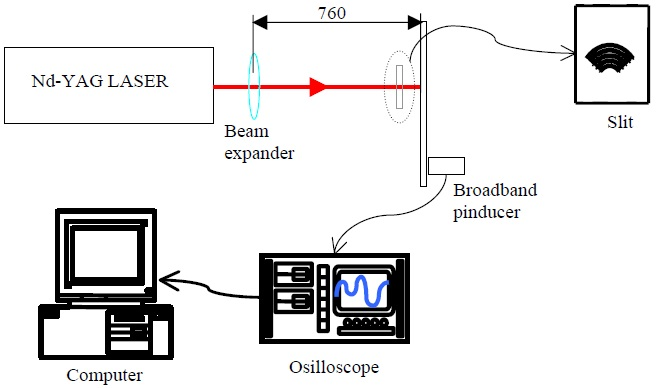
\includegraphics[width=10cm]{Zdjecia/2/laser}
\caption{Przykładowy układ stanowiska do badania fal Lamba w cienkiej płycie \cite{bartek_tian}}
\label{fig:laser}
\end{figure}


%Wzbudzalnosc w sekcji dyspersja

\subsection{Wyznaczanie krzywych wzbudzalności}

Krzywe wzbudzalności określają zależność amplitudy od częstotliwości fali dla poszczególnych jej modów i dla danego wymuszenia. Dla pewnych przypadków można wyznaczyć taką zależność analitycznie, jednak podobnie jak w przypadku krzywych dyspersji, nie jest to metoda uniwersalna. Poniżej znajdują się wyłącznie przykładu numerycznych sposobów wyznaczania tego typu krzywych, ponieważ mają one szersze zastosowanie.

Pierwszy sposób wykorzystuję standardowy model MES ze wzoru \ref{eq:MES1}. Wyznaczamy przemieszczenia węzłów w pewnych chwilach czasowych , a następnie obliczamy wielowymiarowe przekształcenie Fouriera na zgromadzonych danych \ref{eq:fourier_2d}. Wynikiem transformacji jest zależność częstości i liczby falowej, co pozwala wykreślać krzywe dyspersji, a dodatkowo trzecia oś, prostopadła do pozostałych, zawiera informacje o amplitudzie. Przedstawiając na płaszczyźnie zależność amplitudy od liczby falowej, otrzymamy krzywe wzbudzalności.

\vspace{3mm}

Innym sposobem omawianym w literaturze jest zastosowanie metody SAFE (Semi-Analytical Finite Element). Jest ona modyfikacją metody elementów skończonych, polegającą na ustaleniu analitycznego rozwiązania problemu, dla jednego kierunku propagacji. W przypadku problemu trójwymiarowego pozwala to na tworzenie elementów dwuwymiarowych, w kierunkach propagacji, dla których nie znamy rozwiązania. Dzięki temu cały model jest prostszy i szybszy w rozwiązaniu. Sformułowanie takie jest jednak złożone i nie będzie tutaj przytaczane w całości. Jest ono opisane dokładniej w \cite{bartek_fabien}.

Wynikiem wykorzystania metody SAFE jest związek siły wymuszającej i przemieszczenia węzłów modelu. Związek ten przedstawia wzór \ref{eq:wzbudzanie1}. Wzbudzalność określić można na podstawie macierzy E. Określa ona dla modu m, związek pomiędzy siłą przyłożoną w i-tym węźle i przemieszczeniu j-tego węzła \( (\textbf{E}_m)_{ij} \). Rysunek \ref{fig:wzbudzalnosc1} przedstawia wzbudzalność obliczoną dla pierwszych dwóch modów w dwuwarstwowej płycie, bez tłumienia.

\begin{equation} \label{eq:wzbudzanie1}
\textbf{U} = \sum_{m=1}^M \textbf{E}_m \textbf{F}(k_m) e^{ik_m z}
\end{equation}

gdzie
\begin{eqwhere}[2cm]
	\item[$U$] wektor przemieszczenia węzłów
	\item[$E$] macierz wzbudzalności
	\item[$U$] siła wymuszająca w dziedzinie liczby falowej
	\item[$z$] kierunek propagacji, dla którego założono rozwiązanie analityczne
	\item[$m$] numer modu
	\item[$M$] liczba propagujących modów
	\item[$k$] liczba falowa dla m-tego modu.	
\end{eqwhere}

\begin{figure}[h]
\centering
\includegraphics[width=10cm]{Zdjecia/2/wzbudzalnosc1}
\caption{Krzywe wzbudzalności dla dwuwarstwowej cienkiej płyty \cite{bartek_fabien}}
\label{fig:wzbudzalnosc1}
\end{figure}

Kolejna metoda polega na porównaniu prac modów dla fal Lamba z tzw. modem wirtualnym . Prowadzi ona do zależności na wzbudzalność dla cienkich płyt:

\begin{equation} \label{eq:wzbudzanie2}
a_m =  \textbf{X}_m^{(b), H} \frac{\textbf{F}(z)}{i\textbf{P}_{(a:m),(b)}}.
\end{equation}

gdzie

%\begin{equation} \label{eq:wzbudzanie2}
%P_{(a:m),(b)} = \textbf{X}_m^{(b), H} (\textbf{K}_{+1}^{(b),H} e^{-k^{(b)}\Delta x} - \textbf{K}_{-1}^{(b),H} e^{+ik^{(b)}\Delta x} - \textbf{K}_{+1}^{(a)} e^{+ik_m^{(a)}\Delta x} + \textbf{K}_{-1}^{(a)} e^{-ik_m^{(a)}\Delta x})\textbf{X}_{0,m}^{(a)} = 0
%\end{equation}

\begin{equation} \label{eq:wzbudzanie3}
\textbf{P}_{(a:m),(b)} = \textbf{X}_m^{H} (\textbf{K}_{+1}^{H} e^{-ik\Delta x} - \textbf{K}_{-1}^{H} e^{+ik\Delta x} - \textbf{K}_{+1} e^{+ik\Delta x} + \textbf{K}_{-1} e^{-ik\Delta x})\textbf{X}_{0}
\end{equation}

\begin{eqwhere}[2cm]
	\item[$a_m$] amplituda m-tego modu w odpowiedzi na wymuszenie
	\item[$\textbf{F}(z)$] siła wymuszająca działająca wzdłuż grubości płyty
	\item[$\textbf{X}$] wektory własne 
	\item[$\textbf{K}_{\pm 1}$] macierz sztywności dla kolejnej/poprzedniej płaszczyzny propagacji
	\item[$k$] liczba falowa
	\item[$x$] kierunek propagacji
	\item[$m$] numer modu	
	\item[$a_m$] mod numer m, dla pola falowego a
	\item[$b$] mod wirtualny b	
	\item[$H$] sprzężenie hermitowskie.
\end{eqwhere}

Należy zaznaczyć, że do obliczenia amplitud poszczególnych modów, konieczna jest znajomość krzywych dyspersji (zależności \( k(\omega) \) ), oraz wektorów własnych odpowiadających częstościom własnym, dla których wyznaczamy amplitudy.

\subsection{System sing\_around (lub Self-Excited Acoustical System)}

Systemy sing-around to samowzbudne systemy, do pomiaru parametrów rezonansowych fal. Idea systemu polega na dodatnim sprzężeniu zwrotnym pomiędzy przetwornikiem pomiarowym oraz wzbudnikiem. Badanie konstrukcji rozpoczyna arbitralny sygnał wzbudzający. Przetwornik pomiarowy odbiera sygnał i przetwarza go na sygnał elektryczny, który jest odpowiednio filtrowany i wzmacniany, a następnie podawany do wzbudnika. Dane pomiarowe są przesyłane do systemu akwizycji i obróbki, w celu wydobycia informacji o stanie konstrukcji. Schemat przykładowego stanowiska badawczego znajduje się na rysunku \ref{fig:sing_around}.

\begin{figure}[h]
\centering
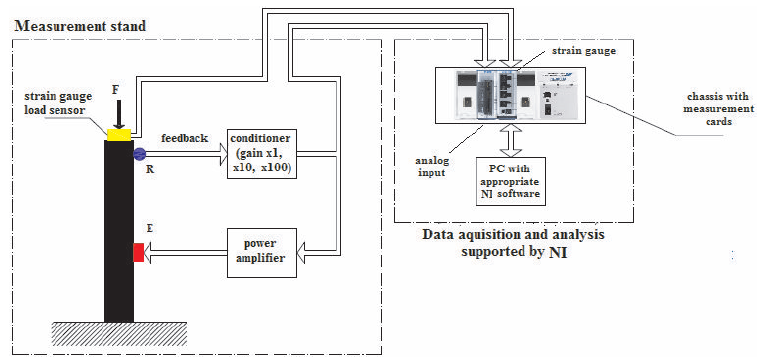
\includegraphics[width=10cm]{Zdjecia/2/sing_around}
\caption{Stanowisko badawcze z systemem sing around \cite{bartek_kwach}}
\label{fig:sing_around}
\end{figure}

Popularnym zastosowaniem tego typu systemów jest pośredni pomiar naprężeń, które mają związek z częstotliwością rezonansową układu bądź prędkością fali, które zmieniają się wraz z odkształcaniem się materiału. Praktycznym przykładem jest pomiar częstotliwości rezonansowej słupa podporowego silosa cementu. Na rysunkach \ref{fig:sing_around_silos} i \ref{fig:sing_around_wyniki} znajduje się widok stanowiska pomiarowego oraz wyniki pomiarów, dla zwiększania i zmniejszania się masy cementu w silosie. W ciągu minuty do silosa dostarczane jest 500kg cementu (125 kg na podporę), a jedno rozładowanie to ok. 2500kg (625 kg na podporę). Przedstawione wyniki dotyczą konfiguracji E1, R1, gdzie E1 to wzbudnik, a R1 to przetwornik pomiarowy.

\begin{figure}[h]
\centering
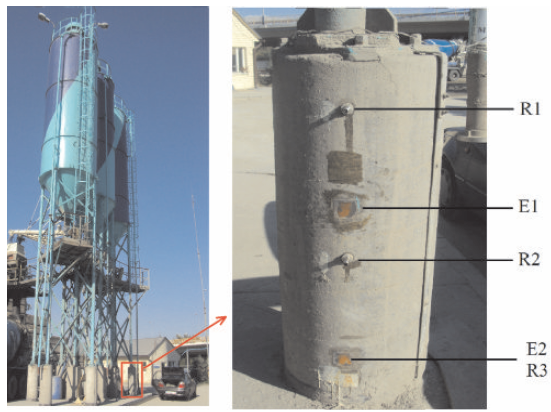
\includegraphics[width=10cm]{Zdjecia/2/sing_around_silos}
\caption{Widok podpory silosa z zamontowanymi przyżadami \cite{bartek_kwach}}
\label{fig:sing_around_silos}
\end{figure}

\begin{figure}[h]
\centering
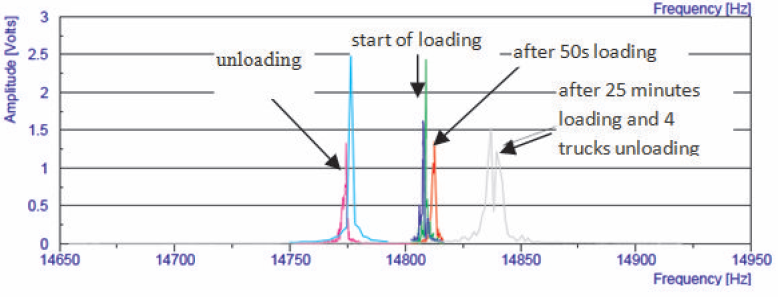
\includegraphics[width=14cm]{Zdjecia/2/sing_around_wyniki}
\caption{Wyniki pomiaru dla ciągłego dostarczania cementu do silosa \cite{bartek_kwach}}
\label{fig:sing_around_wyniki}
\end{figure}

Jak widać częstotliwość rezonansowa zwiększa się wraz ze wzrostem naprężeń ściskających w badanej podporze. Tego typu systemy mają ogromne możliwości zastosowań w różnego typu konstrukcjach, gdzie istotne jest monitorowanie naprężeń.

Znajomość krzywych dyspersji oraz krzywych wzbudzalności dla określonego wymuszenia pozwala zasymulować działanie układu sing-around. Sygnał wyjściowy dla symulacji przebiegu fali, należy podać jako wejście do kolejnej symulacji. Uwzględnienie krzywych dyspersji pozwala określić sposób pomiaru, dla sygnału, który rozbiega się w czasie. Krzywe wzbudzalności pozwalają wyznaczyć piki rezonansowe w widmie badanego sygnału.


%---------------------------------------------------------------------------






















%---------------------------------------------------------------------------





















\chapter{Wykorzystywane zagadnienia metody elementów skończonych}
\chapterauthor{Bartłomiej Piwowarczyk}
\label{cha:MES_chapter}
Metoda elementów skończonych jest zaawansowanym sposobem rozwiązywania równań różniczkowych cząstkowych. Jest ona szczególnym przypadkiem metody Galerkina. Nazwa pochodzi od nazwiska Borisa Grigorievicha Galerkina, który jako pierwszy przeprowadził usystematyzowane studia na temat tego typu metod. Za pomocą tej metody można rozwiązać skomplikowane zadania dziedzin takich jak mechanika ciała stałego, mechanika płynów czy teoria pola elektromagnetycznego. Podstawy tej metody opisane są w \cite{bartek_srodka} oraz \cite{bartek_gavin}. Informacje na temat pochodzenia i estymacji błędów zaczerpnięto z \cite{bartek_pointer} oraz \cite{bartek_erke}.



\section{Rozwiązywanie zadań z  pomocą MES}
\label{sec:rozwiazwyanie_zadan}

W wytrzymałości materiałów poszukujemy zwykle sił działających w poporach konstrukcji i naprężeń wewnątrz jej konkretnych elementów. Innym podejciem jest znalezienie pola przemieszczeń dla każdego punktu konstrukcji.  W jednym i drugim przypadku znalezienie niewiadomych jest osiągalne wyłącznie dla mało skomplikowanych konstrukcji.

Metoda elementów skończonych bierze swoją nazwę od wydzielanych fragmentów konstrukcji, które są właśnie elementami skończonymi. Elementy tworzymy na siatce węzłów, które są punktami wewnątrz lub na brzegach konstrukji. Węzły są także punktami wspólnymi sąsiadujących elementów. Rozwiązanie opiera się na znalezieniu przemieszczenia węzłów i na tej podstawie obliczenia rozwiązania we wszystkich punktach wewnątrz elementów. Kolejne etapy rozwiązywania zadania za pomocą MES przedstawione są poniżej. Rysnuek \ref{fig:MES_przyklad} przedstawia przykład obiektu, który został zdyskretyzowany za pomocą elementów skończonych.

\vspace{5 mm}

\begin{enumerate}
  \item Generacja siatki węzłów.
  \item Budowa elementów skończonych na stworzonej siatce.
  \item Wyznaczanie macierzy mas i sztywności dla każdego elementu (macierze lokalne).
  \item Agregacja macierzy mas  i sztywności dla całej konstrukcji (macierze globalne).
  \item Wprowadzenie wektora obciążeń.
  \item Wprowadzenie warunków brzegowych. Mogą to być siły czynne (modyfikacja wektora obciążeń), naprężenia początkowe czy przemieszczenia wskazanych węzłów.
  \item Rozwiązanie wyznaczonego liniowego równania różniczkowego \( M \ddot x + Kx = F \) - znalezienie przemieszczeń węzłów.
  \item Wyznacznie odkształceń i naprężeń.
  \item Wyznaczenie reakcji w podporach (węzłach, dla których założono przemieszczenie)
\end{enumerate}

\vspace{5 mm}

\begin{figure}[h]
\centering
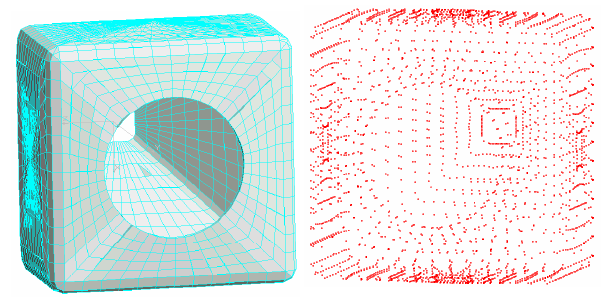
\includegraphics[width=10cm]{Zdjecia/3/MES_przyklad}
\caption{Przykład dsykretyzacji obiektu za pomocą elementów skończonych}
\label{fig:MES_przyklad}
\end{figure}

























\section{Funkcje kształtu}
\label{sec:funkcje_ksztaltu}

Weźmy metalowy pręt o długości L. W punkcie \(x_1\) na pręcie przykładamy temperaturę \( T_1 \), a w punkcie \(x_2\) temperaturę \( T_2 \). Przewidujemy, że po nieskończenie długim czasie rozkład temperatury w pręcie pomiędzy tymi punktami będzie liniowy (Rys. \ref{fig:temperatura_pret}).

\begin{figure}[h]
\centering
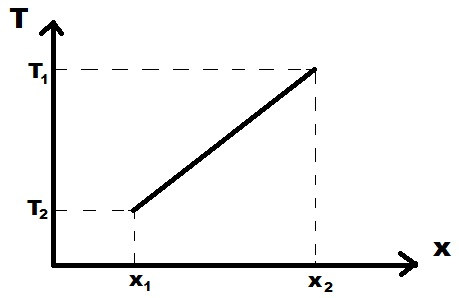
\includegraphics[width=10cm]{Zdjecia/3/rozklad_temperatury}
\caption{Temperatur pomiędzy punktami pręta}
\label{fig:temperatura_pret}
\end{figure}

Temperaturę pomiędzy tymi punktami możemy przedstawić funkcją \ref{eq:funkcja_liniowa}.

\begin{equation} \label{eq:funkcja_liniowa}
T(x)=a_0 + a_1 x, \quad dla \quad x \epsilon [x_1, x_2]
\end{equation}

Można wyznaczyć współczynniki funkcji liniowej mając dwa jej punty.

\begin{equation}
a_1 = \frac{T_2 - T_1}{x_2 - x_1}
\end{equation}

\begin{equation}
a_0 = T_2 - a_1 x_2
\end{equation}

Podstawiając współczyyniki do funkcji, możemy wyznaczyc funkcje kształtu.

\begin{equation}
T(x) = T_1 - \frac{T_2 - T_1}{L} x_1 + \frac{T_2 - T_1}{L} x = \frac{x_2 - x}{L}T_1 + \frac{x - x_1}{L}T_2 = N_1(x)T_1 + N_2(x)T_2
\end{equation}

gdzie
\begin{eqwhere}[2cm]
	\item[$N_1, N_2 $] funkcje kształtu.

\end{eqwhere}

Funkcje kształtu określają w jakim stopniu wartość temperatury z jednego węzła wpływa na wartość temperatury w dowolnym punkcie wewnątrz elementu. Dla większej liczby węzłów w jednowymiarowym elemencie funkcje kształtu są wielomianami wyższych rzędów. Poniżej znajduje się sposób wyznaczania funkcji kształtu na przykładzie 3-węzłowego elementu jednowymiarowego.

\begin{gather} \label{eq:interpolacja}
T(x) = a_0 + a_1 x + a_2 x^2 =
	\begin{bmatrix} 
	 	1 & x& x^2 \\
	\end{bmatrix}
	\begin{bmatrix} 
	 	a_0 \\
		a_1 \\
		a_2 \\
	\end{bmatrix} = \textbf{p} \textbf{a}^e = \textbf{N} \textbf{T}^e
\end{gather}

gdzie
\begin{eqwhere}[2cm]
	\item[$\textbf{p} $] wektor zmiennych kolejnych jednomianów T(x)
	\item[$\textbf{a}^e $] wektor współczynników kolejnych jednomianów T(x)
	\item[$\textbf{N} $] wektor funkcji kształtu
	\item[$\textbf{T}^e $] wektor wartości w węzłach.
\end{eqwhere}

Prawdziwe jest też poniższe równanie.

\begin{gather}
\textbf{T}^e =
	\begin{bmatrix} 
	 	1 & x_1& x_1^2 \\
		1 & x_2& x_2^2 \\
		1 & x_3& x_3^2 \\
	\end{bmatrix}
	\begin{bmatrix} 
	 	a_0 \\
		a_1 \\
		a_2 \\
	\end{bmatrix}
= \textbf{M}^e \textbf{a}^e
\end{gather}

Wyznaczając z tego równania \( \textbf{ a}^e  \) i podstawiając do równania \ref{eq:interpolacja}, otrzymamy następującą zależność.

\begin{equation}
\textbf{p a}^e = \textbf{p} {(\textbf{M}^e)}^{-1} \textbf{T}^e  = \textbf{N T}^e   \quad \Rightarrow \quad \textbf{N} = \textbf{p} {(\textbf{M}^e)}^{-1}
\end{equation}

Funkcje kształtu obliczone w taki sposób mają postać jak poniżej.

\begin{equation}
\begin{aligned}
N_1 = \frac{1}{det\textbf{M}^e} \big(x_2 x_3^2 - x_2^2 x_3 + (x_2^2 - x_3^2)x + (-x_2 + x_3)x^2\big) \\
N_2 = \frac{1}{det\textbf{M}^e} \big(x_1^2 x_3 - x_1 x_3^2 + (x_3^2 - x_1^2)x + (x_1 - x_3)x^2\big) \\
N_3 = \frac{1}{det\textbf{M}^e} \big(x_1 x_2^2 - x_1^2 x_2 + (x_1^2 - x_2^2)x + (-x_1 + x_2)x^2\big)
\end{aligned}
\end{equation}

Prawidłowo wyznaczone funkcje kształtu mają dwi ważną własności. Pierwsza związana jest z węzłami i mówi że każda funkcja przyjmuje wartość 1 w jednym węźle, a we wszystkich pozostałych 0. Druga własność mówi, że suma funkcji kształtu wewnątrz elmentu skończonego wynosi 1. Matematycznie zapisać te własności można następująco:

 \begin{equation} \label{eq:eq_zgodnosc}
	\left\{
                \begin{array}{ll}
		N_n(x_m, y_m) = 1, \quad dla \quad n=m \\
		N_n(x_m, y_m) = 0, \quad dla \quad \neq m 
                \end{array}
	\right.
 \end{equation}

 \begin{equation} \label{eq:WBS}
	\sum_1^n N_n = 1.
 \end{equation}
























\section{Wyznaczanie macierzy sztywności i mas elementów}
\label{sec:wyznaczanie_macierzy}

Weźmy model jednorodnego pręta, obciążonego jak na rysunku \ref{fig:pret} o module Younga \( E \), polu przekroju \( A \) i długości \( L \).

\begin{figure}[h]
\centering
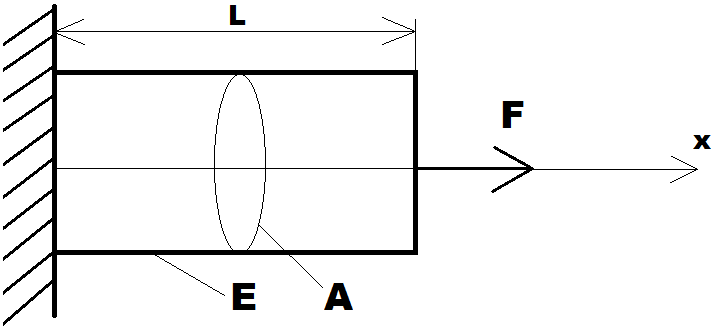
\includegraphics[width=10cm]{Zdjecia/3/pret}
\caption{Model pręta}
\label{fig:pret}
\end{figure}

Energię potencjalną i kinetyczną układu można wyrazić poniższymi wzorami.

\begin{gather} \label{eq:energia}
V = \frac{1}{2} \int_0^L \varepsilon A \sigma dx - Fu_{x=L} = \frac{1}{2} \int_0^L EA {\bigg( \frac{du}{dx}\bigg)}^2 dx - Fu_{x=L} \\
K = \frac{1}{2} \int_0^L \rho A {\bigg(\frac{\partial u}{\partial t}\bigg)}^2 dx
\end{gather}

gdzie
\begin{eqwhere}[2cm]
	\item[$V $] energia potencjalna
	\item[$K $] energia kinetyczna
	\item[$u $] przemieszczenie
	\item[$\varepsilon $] odkształcenie
	\item[$\sigma $] naprężenie
	\item[$F $] siła zewnętrzna skupiona
\end{eqwhere}
	
	Następnie stwórzmy uproszczony model, do którego wyznaczymy zależności MES.

\begin{figure}[h]
\centering
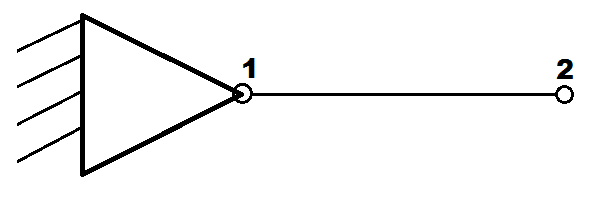
\includegraphics[width=10cm]{Zdjecia/3/pret_upr}
\caption{Uproszczony model pręta}
\label{fig:pret_upr}
\end{figure}

Znając funkcje kształtu i wartości przemieszczeń węzłów można wyznaczyć przemieszczenie w każdym punkcie pręta, a następnie odpowiednie pochodne po przemieszczeniach i po czasie.

\begin{gather}
u = N_1 x_1 + N_2 x_2 = 
	\begin{bmatrix} 
	 	N_1 & N_2 \\
	\end{bmatrix}
	\begin{bmatrix} 
	 	u_1 \\
		u_2 \\
	\end{bmatrix}
\end{gather}

\begin{gather}
\frac{\partial u}{\partial x}= 
	\begin{bmatrix} 
	 	\frac{d N_1}{d x} & \frac{d N_2}{d x} \\
	\end{bmatrix}
	\begin{bmatrix} 
	 	u_1 \\
		u_2 \\
	\end{bmatrix} = \textbf{B u}^e
\end{gather}


\begin{gather}
\frac{\partial u}{\partial t}= 
	\begin{bmatrix} 
	 	N_1 &  N_2 & \\
	\end{bmatrix}
	\begin{bmatrix} 
	 	\frac{du_1}{dt} \\
		\frac{du_2}{dt}\\
	\end{bmatrix} = \textbf{N} \dot{\textbf{u}}^e
\end{gather}


	Mając wyznaczoną energię, możemy obliczyć lagranżjan i wstawić go do dynamicznych równań Lagrangea drugiego rodzaju. Dzięki tej operacji otrzymamy końcowe, dynamiczne równanie ruchu oraz postać macierzy mas i sztywności. Równania Lagrangea drugiego rodzaju mają postać:

\begin{equation}
\frac{d}{dt} \frac{\partial L}{\partial \dot{\textbf{u}}^e} - \frac{\partial L}{\partial \textbf{u}^e} = 0, \quad L = K - V
\end{equation}

gdzie
\begin{eqwhere}[2cm]
	\item[$L$] lagranżjan.
\end{eqwhere}

Pierwszy człon wynosi

\begin{equation}
\frac{d}{dt} \frac{\partial L}{\partial \dot{\textbf{u}}^e} = \int_0^L \rho A {\textbf{N}}^T \textbf{N} {\ddot{\textbf{u}}}^e dx,
\end{equation}

zaś drugi

\begin{equation}
 \frac{\partial L}{\partial \textbf{u}^e} = -\int_0^L EA {\textbf{B}}^T \textbf{B} {\textbf{u}}^e dx + F \textbf{Nu}^e_{x=L}.
\end{equation}

Równanie dynamiki układu zapisane jest poniżej.

\begin{equation}
\int_0^L \rho A {\textbf{N}}^T \textbf{N} dx {\ddot{\textbf{u}}}^e + \int_0^L A {\textbf{B}}^T E \textbf{B} dx u = F \textbf{Nu}^e_{x=L}
\end{equation}

Postaci macierzy mas i sztywności są następujące:

\begin{gather}
\textbf{M}^e = \int_0^L \rho A {\textbf{N}}^T \textbf{N} dx \\
\textbf{K}^e = \int_0^L A {\textbf{B}}^T E \textbf{B} dx.
\end{gather}

W przypadku kiedy występuje więcej niż jedna stała materiałowa, zamiast \( E \) pojawia się macierz materiałowa \( D \). W przypadku bardziej złożonych obiektów o większej liczbie elementów skończonych, całkowanie niezbędne do obliczenia macierzy staje się bardzo czasochłonne. Ponieważ funkcje kształtu są wielomianami, optymalnym rozwiązaniem jest zastosowanie kwadratur Gaussa. Kolejny problem to określenie granic całkowania. W przypadku przedstawionym powyżej nie widać specjalnej trudności, natomiast dla trójwymiarowych obiektów o nieregularnych kształtach wymaga to dodatkowej serii obliczeń.

W takich przypadkach można zastosować mapowanie na współrzędne naturalne. W takich współrzędnych element ma z góry ustalone współrzędne węzłów, co za tym idzie także granice całkowania są znane. Dla obiektu trójwymiarowego przyjmijmy współrzędne rzeczywiste \( x, y, z \) i współrzędne naturalne \( \xi, \eta, \zeta \). Mapowania z jednych współrzędnych na drugie oblicza się według poniższego wzoru. Wizualizacja procedury przedstawiona jest na rysunku \ref{fig:izoparam}.


\begin{gather}
	\begin{bmatrix} 
	 	x \\
		y \\
		z 
	\end{bmatrix} = \sum_{i=1}^n
	\begin{bmatrix} 
	 	x_i \\
		y_i \\
		z_i 
	\end{bmatrix} N_i(\xi, \eta, \zeta)
\end{gather}

\begin{eqwhere}[2cm]
	\item[$x_i, y_i, z_i$] współrzędne rzeczywiste punktów
	\item[$N_i$] funkcje kształtu we współrzędnych naturalnych
	\item[$n$] liczba węzłów elementu.
\end{eqwhere}

\begin{figure}[h]
\centering
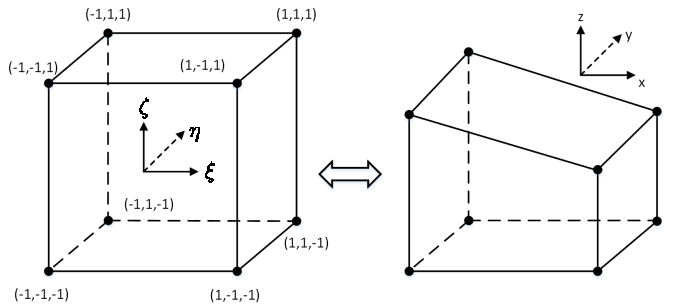
\includegraphics[width=10cm]{Zdjecia/3/izoparam}
\caption{Przekształcenie izoparametryczne}
\label{fig:izoparam}
\end{figure}

Dla elementów w takich współrzędnych funkcje kształtu są znane i stabelaryzowane. Dla elementu sześciennego wypisane są w \ref{eq:f_ksztaltu_hex}.

\begin{equation} \label{eq:f_ksztaltu_hex}
	\begin{aligned}
		N_1 = \frac{1}{8}(1-\xi)(1-\eta)(1-\zeta) \\
		N_2 = \frac{1}{8}(1+\xi)(1-\eta)(1-\zeta) \\
		N_3 = \frac{1}{8}(1+\xi)(1+\eta)(1-\zeta) \\
		N_4 = \frac{1}{8}(1-\xi)(1+\eta)(1-\zeta) \\
		N_5 = \frac{1}{8}(1-\xi)(1-\eta)(1+\zeta) \\
		N_6 = \frac{1}{8}(1+\xi)(1-\eta)(1+\zeta) \\
		N_7 = \frac{1}{8}(1+\xi)(1+\eta)(1+\zeta) \\
		N_8 = \frac{1}{8}(1-\xi)(1+\eta)(1+\zeta)
	\end{aligned}
\end{equation}

Ostatnim elmentem niezbędnym do prawidłowego całkowania we współrzędnych naturalnych jest wyznaczenie jakobianu przekształcenia. Macierz Jacobiego przedstawiona jest w równaniu \ref{eq:m_jacobiego}.

\begin{gather} \label{eq:m_jacobiego}
	\textbf{J} = \begin{bmatrix} 
	 	\frac{\partial x}{\partial \xi} & \frac{\partial y}{\partial \xi} & \frac{\partial z}{\partial \xi} \\
	 	\frac{\partial x}{\partial \eta} & \frac{\partial y}{\partial \eta} & \frac{\partial z}{\partial \eta} \\
	 	\frac{\partial x}{\partial \zeta} & \frac{\partial y}{\partial \zeta} & \frac{\partial z}{\partial \zeta}
	\end{bmatrix}
\end{gather}

Ostatecznie wyznaczanie macierzy mas i sztywności dla elementu sześciennego zostanie zmodyfikowane jak poniżej:

\begin{equation} \label{eq:macierz_sztywnosci}
	\begin{aligned}
	\textbf{K}^e = \int_V {\textbf{B}}^T E \textbf{B} dV \quad \rightarrow \quad \textbf{K}^e =  \int_{-1}^1 \int_{-1}^1 \int_{-1}^1  {\textbf{B}}^T \textbf{D} \textbf{B} det\textbf{J} d\xi d\eta d\zeta.
	\end{aligned}
\end{equation}

\begin{equation} \label{eq:macierz_mas}
	\begin{aligned}
	\textbf{M}^e = \int_V \rho {\textbf{N}}^T \textbf{N} dV \quad \rightarrow \quad \textbf{M}^e = \int_{-1}^1 \int_{-1}^1 \int_{-1}^1 \rho {\textbf{N}}^T \textbf{N} det\textbf{J} d\xi d\eta d\zeta \\
	\end{aligned}
\end{equation}
























\section{Agregacja globalnych macierzy mas i sztywności}
\label{sec:agregacja}

Metoda agregacji macierzy globalnych zostanie przedstawiona na przykładzie macierzy sztywności dwóch elmentów kwadrratowych i obiektu z nich zbudowanego. Wspomniany obiekt przedstawia rysunek \ref{fig:agreg}. Czarne cyfry oznaczają numerację lokalną wewnątrz elmentu, a czerwone numerację globalną.

Algorytm agregacji polega na umieszczaniu odpowiednich elementów macierzy lokalnych do macierzy globalnej. Pokrywające się elementy są sumowane. Ponieważ podmacierz sztywności dla jednego punktu lub zależności pomiędzy punktami jest umieszczana w macierzy globalnej bez wewnętrznych zmian, przyjmijmy zapis uproszczony:

\begin{figure}[h]
\centering
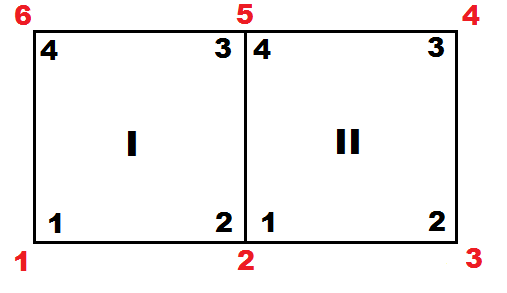
\includegraphics[width=10cm]{Zdjecia/3/agregacja}
\caption{Dwa elementy skończone kwadratowe tworzące obiekt}
\label{fig:agreg}
\end{figure}

\begin{gather}
	\textbf{K}_n^{ij} = \begin{bmatrix} 
	 	K^{ij}_{xx} & K^{ij}_{xy} \\
	 	K^{ij}_{xy} & K^{ij}_{yy} \\
	\end{bmatrix}
\end{gather}

gdzie
\begin{eqwhere}[2cm]
	\item[$i, j$] numery punktów
	\item[$n$] numer elementu
	\item[$x, y$] współrzędne punktów.
\end{eqwhere}

W takim wypadku lokalne macierze sztywności dla obydwu elementów możemy zapisać jako:

\begin{gather}
	\textbf{K}_{I} = \begin{bmatrix} 
	 	\textbf{K}^{11}_I & \textbf{K}^{12}_I & \textbf{K}^{13}_I & \textbf{K}^{14}_I \\
	 	\textbf{K}^{21}_I & \textbf{K}^{22}_I & \textbf{K}^{23}_I & \textbf{K}^{24}_I \\
	 	\textbf{K}^{31}_I & \textbf{K}^{32}_I & \textbf{K}^{33}_I & \textbf{K}^{34}_I \\
	 	\textbf{K}^{41}_I & \textbf{K}^{42}_I & \textbf{K}^{43}_I & \textbf{K}^{44}_I
	\end{bmatrix} \\
	\textbf{K}_{II} = \begin{bmatrix} 
	 	\textbf{K}^{11}_{II} & \textbf{K}^{12}_{II} & \textbf{K}^{13}_{II} & \textbf{K}^{14}_{II} \\
	 	\textbf{K}^{21}_{II} & \textbf{K}^{22}_{II} & \textbf{K}^{23}_{II} & \textbf{K}^{24}_{II} \\
	 	\textbf{K}^{31}_{II} & \textbf{K}^{32}_{II} & \textbf{K}^{33}_{II} & \textbf{K}^{34}_{II} \\
	 	\textbf{K}^{41}_{II} & \textbf{K}^{42}_{II} & \textbf{K}^{43}_{II} & \textbf{K}^{44}_{II}
	\end{bmatrix}.
\end{gather}

Macierze te mają wymiar 8x8, co odpowiada czterem punktom i dwóm współrzędnym dla każdego punktu. Macierz globalna wobec tego będzie miała wymiar 12x12 (6x6 podmacierzy). Poniżej przedstawione jest wyznaczanie kilku elmentów macierzy globalnej.

Dla globalnego punktu 1 mamy:
\begin{equation}
	\textbf{K}^{11} = \textbf{K}_I^{11},
\end{equation}
ponieważ punkt globalny 1 pokrywa się z punktem 1 macierzy I.

Dla globalnego punktu 2 mamy:
\begin{equation}
	\textbf{K}^{22} = \textbf{K}_I^{22} + \textbf{K}_{II}^{11},
\end{equation}
ponieważ punkt globalny 2 pokrywa się z punktem 2 macierzy I oraz punktem 1 macierzy II.

Dla zależności globalnych punktów 2 i 3 mamy:
\begin{equation}
	\textbf{K}^{23} = \textbf{K}_{II}^{12},
\end{equation}
ponieważ punkt globalny 2 pokrywa się z punktem 1, a punkt globalny 3 z punktem 2 macierzy II.

Dla zależności globalnych punktów 2 i 5 mamy:
\begin{equation}
	\textbf{K}^{25} = \textbf{K}_{I}^{23} + \textbf{K}_{II}^{14},
\end{equation}
ponieważ punkt globalny 2 pokrywa się z punktem 2 macierzy I oraz punktem 1 macierzy II, a punkt globalny 5 z punktem 3 macierzy I oraz punktem 4 macierzy II.

Uwzględniając że sztywność względna punktów nie będących ze sobą w sąsiedztwie (np. 1 w pierwszym elemencie oraz 3 w drugim elemencie) wynosi 0, macierz globalna przyjmuje postać:

\begin{gather}
	\textbf{K} = \begin{bmatrix} 
	 	\textbf{K}^{11}_I & \textbf{K}^{12}_I & 0 & 0 & \textbf{K}^{13}_I & \textbf{K}^{14}_I  \\
	 	\textbf{K}^{21}_I & \textbf{K}^{22}_I + \textbf{K}^{11}_{II}  & \textbf{K}^{12}_{II} & \textbf{K}^{13}_II & \textbf{K}_{I}^{23} + \textbf{K}_{II}^{14} & \textbf{K}^{24}_I \\
	 	0 & \textbf{K}^{21}_{II} & \textbf{K}^{22}_{II} & \textbf{K}^{23}_{II} & \textbf{K}^{24}_II & 0 \\
	 	0 & \textbf{K}^{31}_II & \textbf{K}^{32}_{II} & \textbf{K}^{33}_{II} & \textbf{K}^{34}_{II} & 0 \\
		\textbf{K}^{31}_I & \textbf{K}_{I}^{32} + \textbf{K}_{II}^{41} & \textbf{K}^{42}_II & \textbf{K}^{43}_{II} & \textbf{K}^{33}_{I} + \textbf{K}	^{44}_{II} & \textbf{K}^{34}_{I} \\
		\textbf{K}^{41}_I & \textbf{K}^{42}_I & 0 & 0 & \textbf{K}^{43}_I & \textbf{K}^{44}_I.
	\end{bmatrix}
\end{gather}

Oczywistym jest, że w przypadku innej numeracji węzłów globalnych zmieni się układ macierzy globalnej. Nie ma to jednak wpływu na ostateczny wynik rozwiązania MES. W modelach o dużej liczbie elmentów skończonych macierze mas i sztywności są macierzami rzadkimi. Wykorzystuje się to w obliczeniach do oszczędzania pamięci komputera, poprzez zapis w pamięci tylko wartości niezerowych oraz ich położenia w macierzy. 

Macierz mas wyznaczona w przedstawiony sposób jest nazywana macierzą konsystentną. Często stosuje się macierze skupione, które zawierają elementy tylko na diagonali. Pozwala to bardzo przyspieszyć obliczenia. Takie rozwiązanie jest ściśle rzecz biorąc niepoprawne, ponieważ nie ma algorytmu, który pozwala obliczyć macierz skupioną i zachować w pełni właściwości modelu. Macierze skupione oblicza się np. poprzez sumowanie wszystkich elmentów w wierszu i umieszczanie tej sumy na elemencie diagonalnym. Dobrą stroną macierzy skupionych jest fakt, że rozwiązanie pozostaje zbieżne.






















\section{Rozwiązanie wyznaczonego równania macierzowego}
\label{sec:rozwiazanie_r_roz}

Przyjmijmy, że wyznaczone równanie różniczkowe po agregacji macierzy ma postać:

\begin{equation} \label{eq:mes_wyjsciowe}
	\textbf{M} \ddot{\textbf{x}} + \textbf{Kx} = \textbf{F}.
\end{equation}

Rozwiązać to równanie można na wiele sposobów. Przedstawione zostaną tutaj trzy. Pierwszy sposób to metoda całkowania jawnego, druga - metoda całkowania niejawnego, a trzecie to metoda modalna.

W metodzie całkowania jawnego zakładamy rozpoczęcie obliczeń w kroku czasowym t i przybliżamy pochodną drugiego rzędu poprzez formułę centralną:

\begin{equation}
	\ddot{\textbf{x}}^t = \frac{\textbf{x}^{t+1} - 2\textbf{x}^t + \textbf{x}^{t-1}}{\delta t^2}.
\end{equation}

Po podstawieniu do równania \ref{eq:mes_wyjsciowe} wyznaczamy \( \textbf{x}^{t+1} \):

\begin{equation} \label{eq:jawne_calkowanie}
	\textbf{x}^{t+1} = \Delta t^2 \textbf{M}^{-1}(\textbf{F}^t - \textbf{Kx}^t) + 2\textbf{x}^t - \textbf{x}^{t-1}.
\end{equation}

Metoda ta charakteryzuje się tym, że do stabilności rozwiązania często wymaga małego kroku czasowego. Nadaje się ona za to do zrównoleglania obliczeń, co pozwala zastosować do tego celu procesory graficzne. Operacja odwracania macierzy \( \textbf{M} \) we wzorze \ref{eq:jawne_calkowanie} jest kosztowna obliczeniowo. Zastosowanie macierzy skupionej pozwala znacznie przyspieszyć tą procedurę.

Metoda całkowania niejawnego różni się wyjściowym krokiem czasowym. Zakładamy początkową chwilę czasową \( t+1 \), co przy zastosowaniu tej samej formuły różnicowej wprowadza krok wstecz.

\begin{equation} \label{eq:niejawne}
	\ddot{\textbf{x}}^{t+1} = \frac{\textbf{x}^{t+1} - 2\textbf{x}^t + \textbf{x}^{t-1}}{\delta t^2}.
\end{equation}

Podstawiamy równanie \ref{eq:niejawne} do równania

\begin{equation} \label{eq:mes_wyjsciowe}
	\textbf{M} \ddot{\textbf{x}}^{t+1} + \textbf{Kx}^{t+1} = \textbf{F}^{t+1}
\end{equation}

i otrzymujemy 

\begin{equation} 
	\textbf{x}^{t+1} = (\textbf{M} + \Delta t^2 \textbf{K})^{-1} (\Delta t^2 \textbf{F}^{t+1} + 2\textbf{MX}^t - \textbf{MX}^{t-1}.
\end{equation}

W tym wypadku nie unikniemy już odwracania macierzy \( \textbf{M} + \Delta t^2 \textbf{K} \), co powoduje wydłużenie obliczeń. Zaletą tej metody jest fakt, że jest ona bezwarunkowo stabilna.

W metodzie modalnej jako pierwsze należy wyznaczyć wektory własne dla równania jednorodnego \( \textbf{M} \ddot{\textbf{x}} + \textbf{Kx} = 0 \). Wektory własne wyznaczyć można z dokładnością do stałej multiplikatywnej. Możliwe jest wyskalowanie tych wektorów w taki sposób, aby maciesz tych wektorów \( \boldsymbol{\phi} \) miała własność:

\begin{equation} 
	\boldsymbol{\phi}^T \textbf{M} \boldsymbol{\phi} = \textbf{I}.
\end{equation}

Zakładając przekształcenie współrzędnych \( \textbf{x} = \boldsymbol{\phi} \overbar{\textbf{x}}  \) otrzymamy nową postać równania \ref{eq:mes_wyjsciowe}.

\begin{equation} 
	\ddot{\overbar{\textbf{x}}} + \boldsymbol{\Lambda} \overbar{\textbf{x}} = \overbar{\textbf{F}}, \quad \boldsymbol{\Lambda} = \boldsymbol{\phi}^T\textbf{K}\boldsymbol{\phi}, \quad \overbar{\textbf{F}} = \boldsymbol{\phi}^T \textbf{F}.
\end{equation}

Macierz \( \boldsymbol{\Lambda} \) jest macierzą diagonalną, więc rozwiązanie układu sprowadza się teraz do znalezienia rozwiązania dla pojedynczych oscylatorów harmonicznych. Elementy macierzy \( \boldsymbol{\Lambda} \) są kwadratami częstości własnych drgań węzłów.

\begin{gather}
	\begin{bmatrix} 
		\ddot{\overbar{x}_1} \\
		\ddot{\overbar{x}_2} \\
		\ddot{\overbar{x}_3} \\
		\vdots \\
		\ddot{\overbar{x}_n}
	\end{bmatrix} +
	\begin{bmatrix} 
		\omega_1^2	&			&			&				& \\
				& \omega_2^2	& 			& \text{\huge{0}}		& \\
				&			& \omega_3^2 	& 				& \\
				& \text{\huge{0}}	& 			& \ddots			& \\
				&			&			&				& \omega_n^2
	\end{bmatrix}
	\begin{bmatrix} 
		\overbar{x}_1 \\
		\overbar{x}_2 \\
		\overbar{x}_3 \\
		\vdots \\
		\overbar{x}_n
	\end{bmatrix} =
	\begin{bmatrix} 
		\overbar{F}_1 \\
		\overbar{F}_2 \\
		\overbar{F}_3 \\
		\vdots \\
		\overbar{F}_n
	\end{bmatrix}
\end{gather}

 \begin{equation}
	\left\{
                \begin{array}{ll}
  		\ddot{\overbar{x}_1}+\omega_1^2\overbar{x}_1=\overbar{F}_1 \quad \rightarrow\\
  		\ddot{\overbar{x}_2}+\omega_2^2\overbar{x}_2=\overbar{F}_2 \quad \rightarrow\\
  		\ddot{\overbar{x}_3}+\omega_3^2\overbar{x}_3=\overbar{F}_3 \quad \rightarrow\\
		\quad \quad \vdots \quad \quad \\
  		\ddot{\overbar{x}_n}+\omega_n^2\overbar{x}_n=\overbar{F}_n \quad \rightarrow
                \end{array}
	\begin{bmatrix} 
		\overbar{x}_1 \\
		\overbar{x}_2 \\
		\overbar{x}_3 \\
		\vdots \\
		\overbar{x}_n
	\end{bmatrix}
	\right.
 \end{equation}

Po rozwiązaniu równań należy wyznaczyć ostateczne rozwiązanie \( \textbf{x} = \boldsymbol{\phi} \overbar{\textbf{x}}  \).




















\section{Zbieżność metody i błędy rozwiązania}
\label{sec:zbieznosc_i_blad}

O zbieżności rozwiązania możemy wnioskować na podstawie funkcji kształtu. Pierwszym warunkiem jest tzw. warunek zgodności. Mówi on o tym, że funkcje kształtu muszą być ciągłe w przestrzeni elementów. Dla prostego przypadku dwóch elementów liniowych jednowymiarowych ciągłość funkcji ilustruje rysunek \ref{fig:zgodnosc}. 

\begin{figure}[h]
\centering
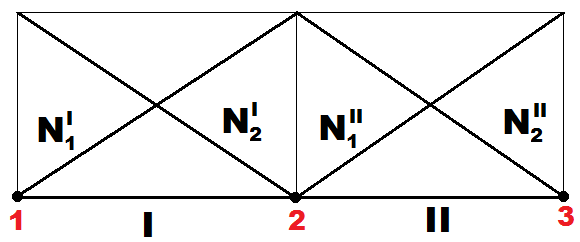
\includegraphics[width=10cm]{Zdjecia/3/zgodnosc}
\caption{Ciągłość funkcji w przestrzenii elementów}
\label{fig:zgodnosc}
\end{figure}

Warunek ten jest zapewniony poprzez własność funkcji kształtu przedstawioną we wzorze \ref{eq:eq_zgodnosc}.

Kolejny warunek nazywa się warunkiem bryły sztywnej (WBS). Zapewnia on brak straty bądź narastania energii podczas wyznaczania wyniku wewnątrz elementu. Warunek ten jest zapewniony poprzez własność funkcji kształtu przedstawioną w \ref{eq:WBS}.

Ostatnim warunkiem jest tzw. warunek stałego odkształcenia (WSO). Mówi on o tym, że jeśli w elemencie przyłożymy liniowe pole przemieszczeń, to odkształcenie będzie stałe w każdym punkcie elementu.

Jeśli spełnione są warunki zgodności, WBS oraz WBO to rozwiązanie dla elementu będzie zbieżne. Warunki te muszą być spełnione dla każdego elementu obliczanego modelu.

\vspace{3mm}

Zbieżność nie daje nam gwarancji, że rozwiązanie otrzymane przy pomocy symulacji MES jest poprawne. Przez poprawne rozumiane jest, że błąd rozwiązania jest dostatecznie mały. Aby mieć pewność, że rozwiązanie jest wystarczająco dokładne należy oszacować błąd maksymalny. W przypadku MES błąd powodują:

\begin{enumerate}
	\item dyskretyzacja konstrukcji 
	\item zaokrąglenia arytmetyczne.
\end{enumerate}

\vspace{3mm}

Pierwsza przyczyna występowania błędów związana jest z podziałem konstrukcji na elementy skończone. Błąd zawarty jest już w równaniu \( \textbf{M} \ddot{\textbf{x}} + \textbf{Kx} = \textbf{F} \). Pojawia się dlatego, że całe rozwiązanie wyznaczamy za pomocą wielomianowych funkcji kształtu. Błąd zbieżnego rozwiązania możemy zmniejszać poprzez wykorzystanie funkcji kształtu wyższego rzędu, bądź zagęszczenie siatki i budowę większej liczby elementów skończonych.

Estymacja błędów odbywa się na różne sposoby. Jednym z nich jest wykorzystanie równania \ref{eq:blad1}. 

\begin{equation} \label{eq:blad1}
	F - \tilde{F}_i \approx ch_i^r
\end{equation}

gdzie
\begin{eqwhere}[2cm]
	\item[$ F $] rozwiązanie dokładne
	\item[$ \tilde{F}_i $] i-te rozwiązanie przybliżone
	\item[$ c $] współczynnik proporcjonalności
	\item[$ h_i $] współczynnik zależny od zagęszczenia siatki
	\item[$ r $] współczynnik zależny od stopnia wielomianów interpolujących.
\end{eqwhere}

Jedna symulacja nie daje możliwości wyznaczyć błędu. Aby tego dokonać należy przeprowadzić dwie symulacje, co pozwala obliczyć błąd drugiej (dokładniejszej). Przyjmijmy, że druga symulacja zawiera elementy o dwukrotnie mniejszych wymiarach, czyli \( h_1 = 2h_2 \). Współczynnik \( r \) przyjmuje wartości mniejsze od 1, ale dla uproszczenia przyjmijmy dokładnie 1.

Podstawiając odpowiednie indeksy do wzoru \ref{eq:blad1}, możemy wyznaczyć błąd drugiej symulacji, znając wyniki zarówno pierwszej jak i drugiej.

\begin{equation} 
	F- \tilde{F}_2 \approx \frac{\tilde{F}_2 - \tilde{F}_1}{(\frac{h_1}{h_2})^r - 1}.
\end{equation}

Innym podejściem jest wyznaczanie błędów poprzez energię naprężenia elementów. Po wyznaczeniu przemieszczeń węzłów i obliczeniu naprężeń, naprężenia nie są ciągłe w przestrzeni elementów. Jeśli jeden węzeł należy do kilku elementów, to w każdym z nich może zostać wyznaczona inna wartość naprężenia dla takiego węzła. W ciągłym przypadku naprężenie byłoby funkcją ciągłą, dlatego błąd wynikający z naprężeń wyznacza się w następujący sposób:

\vspace{3mm}

\begin{enumerate}
	\item Obliczamy średnią naprężeń w węźle, biorąc wartości dla węzła z każdego elementu, do którego należy.
	\item Wyznaczamy błąd naprężenia w węzłach elementu, poprzez odejmowanie od naprężenia w węźle wartości średniego naprężenia w tym węźle.
	\item Sumujemy błędy naprężeń wszystkich elementów skończonych.
	\item Wyznaczamy energię błędu naprężenia.
	\item Wyznaczamy energię odkształcenia dla całej konstrukcji.
	\item Obliczamy błąd procentowy według wzoru \ref{eq:blad2}.
\end{enumerate}

\vspace{3mm}

\begin{equation} \label{eq:blad2}
	E = 100(\frac{e}{U + e})^{0.5}
\end{equation}

gdzie
\begin{eqwhere}[2cm]
	\item[$ e $] całkowita energi błędu dla konstrukcji
	\item[$ U $] energi odkształcenia dla konstrukcji
	\item[$ E $] błąd procentowy energii.
\end{eqwhere}













































\chapter{Metody kompensacji dyspersji}
\label{cha:comp_disp}
 
Istnieje wiele różnych metod kompensacji dyspersji w tej pracy szczegółowo opisane zostały wybrane trzy. Pierwsza polegająca na przygotowaniu sygnału, który sam skompensuje się do odpowiedniej postaci w trakcie propagacji. Druga bazująca na przybliżaniu krzywych dyspersji przy pomocy rozwinięcia w szereg Taylora, oraz trzecia polegająca na mapowaniu sygnału z dziedziny czasu na odległość 
 

\section{Cel kompensacji}
\label{sec:cel_komp}

\subsection{Zastosowanie fal Lamba w nieniszczacych testach}

Fale prowadzone akustyczne i ultradźwiękowe, w tym między innymi fale Lamba, są wykorzystywane na wiele sposobów między innymi do nieniszczących testów oraz oceny jakości obiektów. Stosowane są między innymi do diagnostyki uszkodzeń aktywnych lub pasywnych w monitorowaniu kondycji strukturalnej (SHM - Structural Health Monitoring). W niektórych przypakach fale te są wykorzystywane do uzyskania lokalnych informacji o próbce, której to informacji nie można uzyskać konwencjonalnymi technikami ultradźwiękowymi. Przykładem takiego zastosowania może być inspekcja spoiwa klejowego[2-Wilcox]. Jest to przykład aplikacji o krótkim zasięgu, ponieważ odległość propagacji fal kierowanych jest stosunkowo mała. Drugi obszar zastosowania kontroli fal prowadzonych jest przeznaczony do testowania dalekiego zasięgu. W tym przypadku odległość propagacji jest stosunkowo duża. Ich główną zaletą, sprawiającą, iż są one tak często wykorzystywane do diagnozy urządzeń jest to, że mogą być wzbudzane przez elementy uruchamiające znajdujące się na lub wewnątrz struktury w jednym punkcie konstrukcji i mogą się rozprzestrzeniać na duże odległości. Konwencjonalna kontrola ultradźwiękowa dużych struktur jest bardzo czasochłonna, ponieważ testom musi zostać poddany każdy punkt badanej struktury, która ma być monitorowana. Wykorzystanie fal Lamba jest więc potencjalnie bardzo atrakcyjnym rozwiązaniem tego problemu. Jeżeli przetwornik odbierający znajduje się w odległym punkcie struktury, odebrany sygnał zawiera informacje o całej przebytej ścieżce propagacji między przetwornikami nadawczym i odbiorczym. W związku z tym test monitoruje całą ściężkę, a nie pojedynczy punkt struktury. Pozwala to na znaczne zaoszczędzenie czasu badań. W przypadku prętów niejednokrotnie stosuje się techniki, w których nadajnik po wyemitowniu sygnału przełącza się w tryb odbiornika. Propagujący sygnał odbija się od końca pręta i wraca spowrotem, gdzie jest odbierany i może zostać poddany analizie. Takie podejście jest bardzo często stosowane, zwłaszcza w sytuacjach, w których dostęp do pręta możliwy jest tylko z jednej strony jak na przykład podczas badania kotw górniczych. Przykład ich położenia ilustruje rysunek \ref{fig:kotwy}
\begin{figure}[h]
\centering
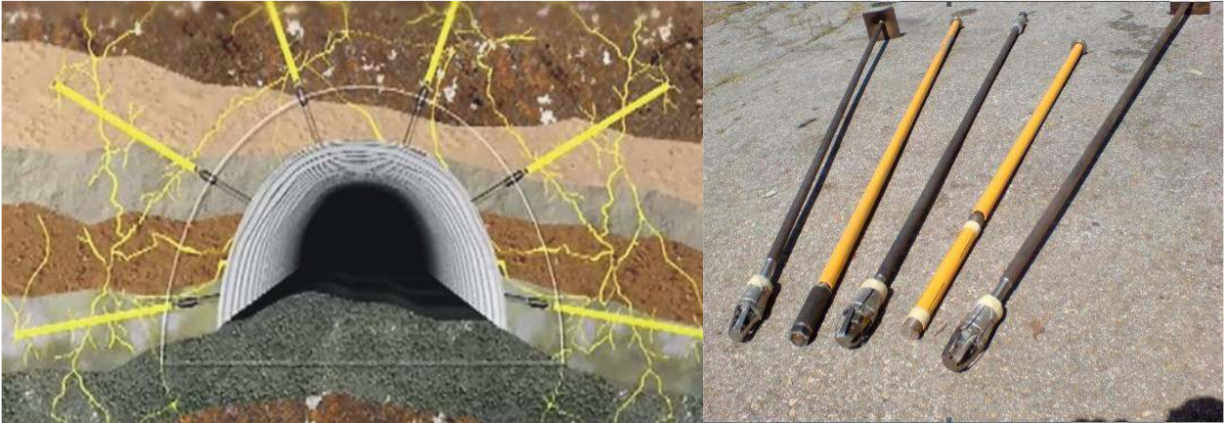
\includegraphics[width=14cm]{Zdjecia/4/kotwy}
\caption{Przykład zamontowania kotw górniczych, do których dostęp w przypadku testów jest tylko z jednej strony \ref{art:kotwy}}
\label{fig:kotwy}
\end{figure}

Nawet w najprostszych strukturach, takich jak swobodna płaska izotropowa płyta lub prosty stalowy pręt, może istnieć nieskończona liczba sterowanych trybów falowych. Co więcej, postaci te są generalnie dyspersyjne. Obydwa te fakty utrudniają praktyczne zastosowanie fal kierowanych. W praktyce testy kontroli dalekiego zasięgu są wykonywane w sposób zadowalający, gdy stosuje się tylko jedną lub czasami dwie postaci fal prowadzonych, a pozostałe są tłumione. Tradycyjnie osiąga się to za pomocą specjalnych przetworników. Dzięki starannej kontroli częstotliwości i liczby falowej wzbudzenia, możliwe jest generowanie wybranych postaci fali Lamba oraz tłumienie pozostałych. Kontrola zakresu częstotliwości może być osiągnięta przez użycie sygnału o pewnej szerokości pasma zamkniętego w oknie Hanninga lub Gaussa. Zakres liczby falowej może być ograniczony przez użycie starannie zaprojektowanych sond EMAT lub za pomocą piezoelektrycznego przetwornika. 

Powyższe metody mogą służyć do tłumienia sygnałów wywołanych przez niepożądane postaci fali, ale nie mogą zapobiec efektowi dyspersji, ponieważ zjawisko to występuje w falach kierowanych podczas ich propagacji w strukturze. Dyspersja sygnału powoduje, rozproszenie energii sygnału w czasie i przestrzeni w trakcie propagacji sygnału. W praktyce objawia się to wzrostem czasu trwania odbieranego sygnału w porównaniu do czasu trwania sygnału wejściowego. Rysunek \ref{fig:dyspersja} ilustruje przykład sygnału bez dyspersji oraz sygnału rozproszonego na skutek propagacji pewnej odległości. Łatwo zauważyć, że sygnał przed propagacją trwa zaledwie $0,0001 s$ natomiast po jego czas zwiększa się do około $0,0013s$ a zatem trwa ponad 10 razy dłużej.
\begin{figure}[h]
\centering
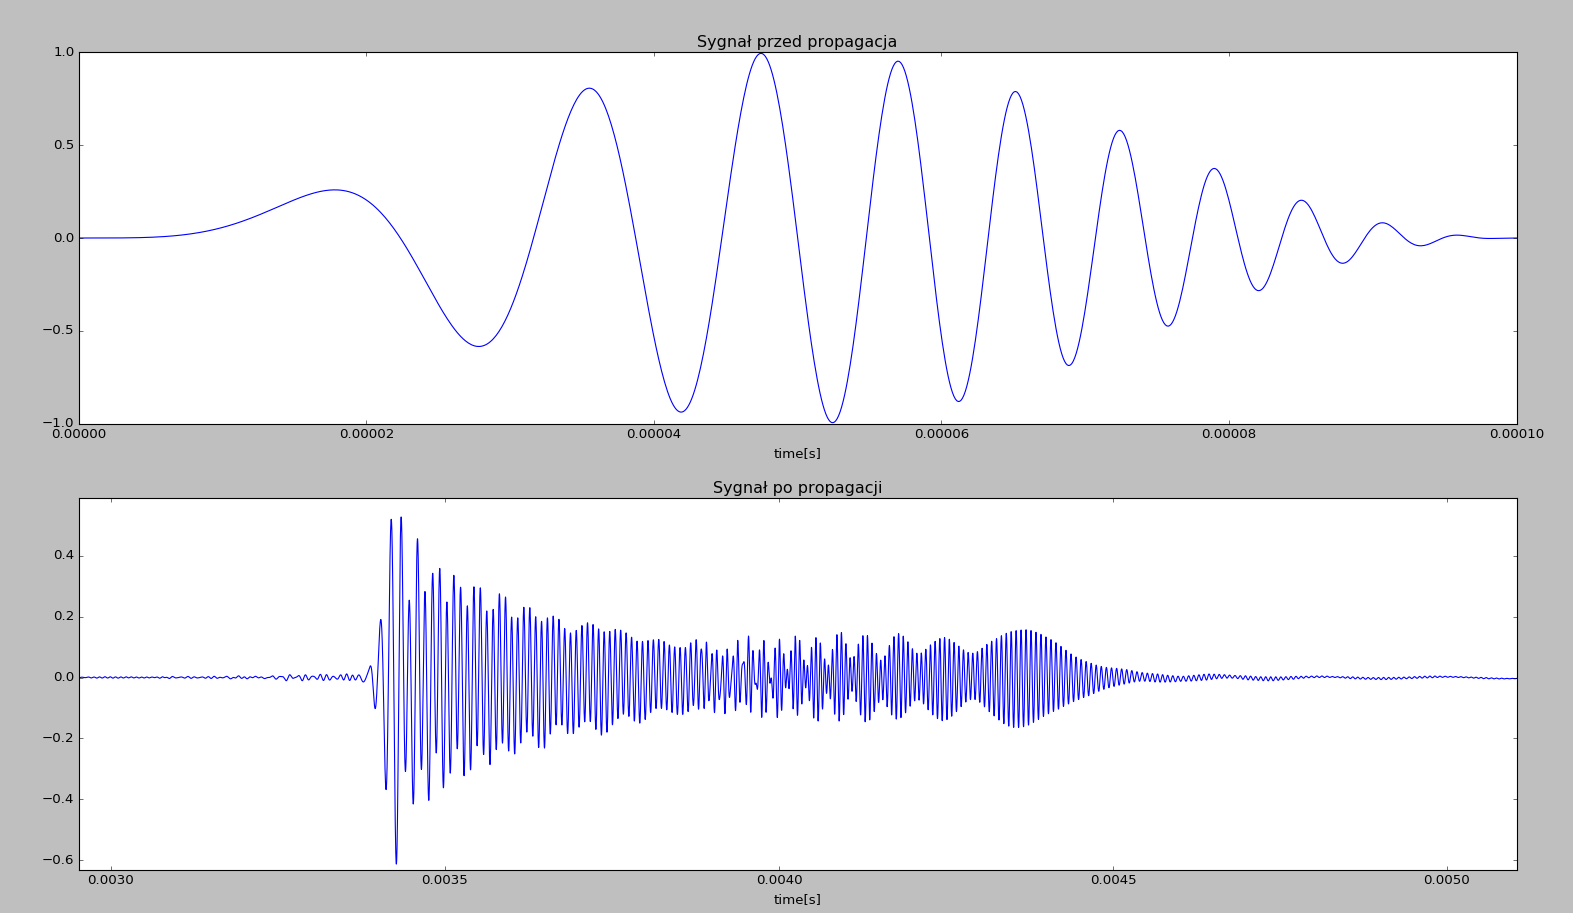
\includegraphics[width=14cm]{Zdjecia/4/dyspersja}
\caption{Przykład sygnału wejściowego, oraz sygnału rozproszonego}
\label{fig:dyspersja}
\end{figure}

 Zjawisko to pogarsza rozdzielczość i sprawia, że dane eksperymentalne są trudne do interpretacji z powodu nakładania się sygnałów. Używanie sygnałów wejściowych o określonej przepustowości może zmniejszyć problem dyspersji. Takie podejście koncentruje energię wejściową w ograniczonym zakresie częstotliwości, w którym jakiekolwiek zmiany prędkości pożądanego trybu fal kierowanych są małe. W praktyce oznacza to pracę w punktach na krzywych dyspersji dla konkretnego układu, w których prędkość grupowa jest stacjonarna lub prawie stacjonarna względem częstotliwości. Takie punkty zostały określone jako punkty "zerowej dyspersji" w\textcolor{red}{[1kasia]}, jest to określenie, które może wprowadzać w błąd, ponieważ niemożliwe jest skoncentrowanie całej energii sygnału wejściowego o skończonej długości na jednej częstotliwości. Zostało udowodnione \textcolor{red}{[2kasia]}, że istnieje optymalny sygnał wejściowy dla każdego punktu na krzywych dyspersji, który maksymalizuje rozdzielczość, jaką można uzyskać w tym punkcie. Jeśli jednak przyjmiemy, że przetwarzanie sygnału jest dozwolone przed wyświetlaniem informacji operatorowi, możliwe jest inne podejście do fal prowadzonych oraz ich roli w nieniszczących testach.

Należy również zaznaczyć, iż w praktyce rozproszone sygnały są zwykle uszkodzone z powodu szumów. Zachodzące na siebie i słabnące sygnały w porównaniu z szumem sprawiają, że dane z czujników są trudniejsze do interpretacji. W konsekwencji rodzielczość może ulec pogorszeniu. Dlatego zrodziła się ogromna potrzeba opracowania technik przetwarzania sygnałów w celu zwiększenia rozdzielczości czasowej i amplitudy SNR.

Z punktu widzenia systemów SHM, kompresja sygnału lub usuwanie dyspersji w dziedzinie czasu może być wygodnym i intuicyjnym sposobem na łatwiejszą interpretację sygnałów czujnika.

\subsection{Sygnał stosowany wy symulacji}
W ramach niniejszej pracy powstała aplikacja, pozwalająca użytkownikowi na podstawie podanych parametrów pręta wygenerować krzywe dyspersji opisujące dany obiekt. Aplikacja pozwala również na wygenerowanie sygnału testowego, symulację jego propagacji w zadanym pręcie, oraz kompensację otrzymanego sygnału wybranymi metodami. Sygnałem stosowanym do testów był sygnał chirp zmodyfikowany przypomocy okna Hanninga.
	Sygnał o nazwie chirp jest sygnałem sinusoidalnym, w którym faza jest funkcją czasu. \textcolor{red}{[3kasia]}. Sygnał o nazwie linear chirp to sygnał, w którym częstotliwość zmienia się w sposób liniowo zależny od czasu. Sygnał taki jest opisany wzorem:
	\begin{equation}
	s(t) = \sin(\phi (t))
	\end{equation}
	
	Gdzie $\phi (t)$ to funkcja fazy. Chwilową częstotliwość takiego sygnału jest związana funkcją fazy następującą zależnością:
	\begin{equation}
	f(t) = \frac{1}{2\pi}\frac{d(\phi (t))}{dt} \label{eq:f(t)_z_phi}
	\end{equation}
	
	Aby zatem wygenerować sygnał linear chirp o rządanych parametrach należy przyjąć, iż funkcja częstotliwości przybiera postać:
	\begin{equation}
	f(t) = f_0+\frac{B}{T}t \label{eq:f(t)_liniowo}
	\end{equation}
	
	Gdzie:
	
	$f_0$ - częstotliwość początkowa
	
	$B$ - szerokość pasma częstotliwości
	
	$T$ - czas trwania sygnału
	
	Łącząc równania (\ref{eq:f(t)_z_phi}) oraz (\ref{eq:f(t)_liniowo}) można funkcję fazy zapisać jako:
	\begin{equation}
	\phi (t) = 2\pi f_0t+\frac{\pi Bt^2}{T} \label{eq:phi(t)}
	\end{equation}
	A zatem pełen wzór opisujący sygnał linear chirp można zapisać jako:
	\begin{equation}
	s(t) = \sin(2\pi f_0t+\frac{\pi Bt^2}{T})
	\end{equation}
	
	Przykład funkcji częstotliwości oraz uzyskanego w ten sposób sygnału przedstawia rysunek \ref{fig:linear_chirp}
\begin{figure}[h]
\centering
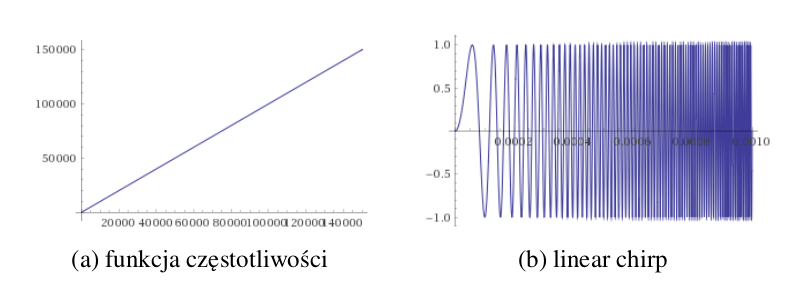
\includegraphics[width=14cm]{Zdjecia/4/linear_chirp}
\caption{Przykład sygnału linear chirp (b) oraz jego funkcji częstotliwości (a)}
\label{fig:linear_chirp}
\end{figure}

W prezentowanej pracy, sygnałem, który był poddawany symulacji był liniowy chirp dodatkowo pomnożony przez funkcję okna Hanninga daną wzorem:
\begin{equation}
w(n)=0,5(1-cos(\frac{2\pi n}{N-1})) \label{eq:okno_hanninga}
\end{equation}

Gdzie $N$ to całkowita liczba próbek. uzyskany w ten sposób sygnał został zaprezentowany na rysunku \ref{fig:test_chirp}
\begin{figure}[h]
\centering
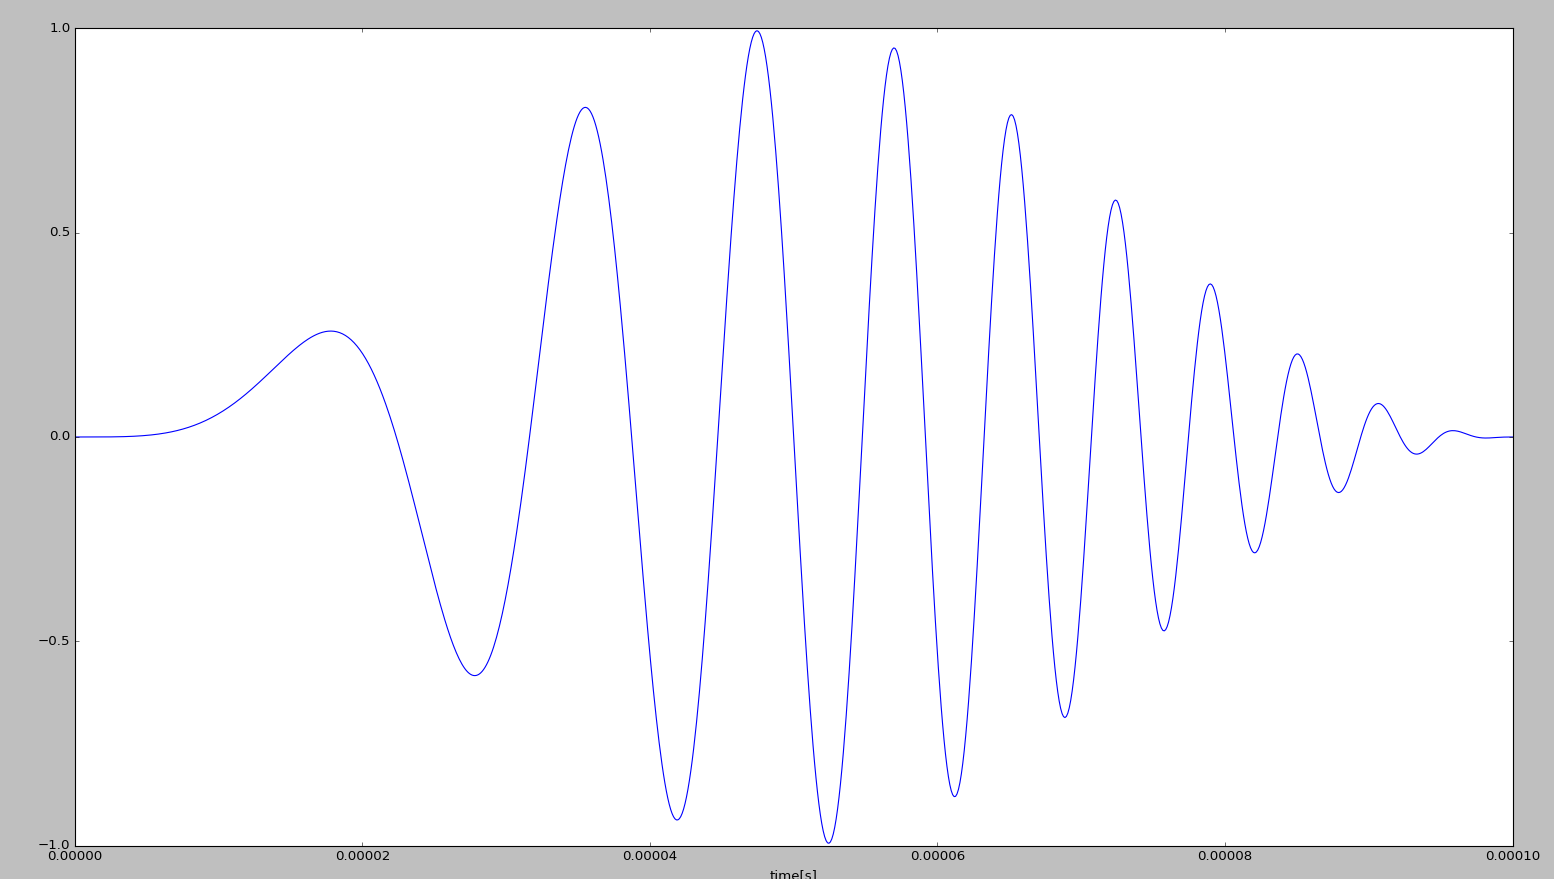
\includegraphics[width=14cm]{Zdjecia/4/test_chirp}
\caption{Linear chirp pomnożony przez funkcję okna Hanninga}
\label{fig:test_chirp}
\end{figure}

W aplikacji zaimplementowany został algorytm generujący opisany wyżej sygnał o następujących parametrach:

\begin{itemize}
\item czas trwania sygnału - 0.0001s
\item częstotliwość minimalna - 0Hz
\item częstotliwość maksymalna - 100kHz
\end{itemize}

Całość stworzona jest w oparciu o koncepcję otwartego koduco daje użytkownikowi możliwość pisania własnych funkcji, generujących dowolne sygnały a następnie ich bezproblemową symulcję w stworzonej aplikacji.

\section{Agregacja krzywych dyspersji uzyskanych z zaimplementowanego solvera}
\label{sec:agregacja}

\subsection{Cel agregacji}
Podstawą opracowania każdej z przedstawionych w tej pracy metod kompensacji jest znajomość krzywych dyspersji badanego obiektu, jakim jest stalowy pręt. Stanowią one pewnego rodzaju funkcję przejścia sygnału pomiędzy jednym punktem w czasie i przestrzeni a dowolnym innym punktem. Ich znajomość stanowi więc klucz do skompensowania efektu dyspersji. W stworzonej aplikacji, dzięki zastosowaniu odpowiednich algorytmów oraz na podstawie odpowiednich zadanych parametrów badanego obiektu, otrzymywane są poszukiwane krzywe dyspersji. Jednak dane są one w postaci chmury punktów zapisywanych w odpowiednich plikach. Aby funkcje te nadawały się do użycia należy każdy z wygenerowanych punktów przypisać do odpowiadającej krzywej. W ten sposób uzyskane zostaną funkcje, z których każda opisywać będzie zachowanie innej postaci fali prowadzonej. Przykładowe wygenerowane krzywe dyspersji przed agregacją przedstawia rysunek 2.21

\subsection{Algorytm agregacji}
 Krzywe dyspersji wyrażają zależność liczby falowej od częstości kątowej. Jako wynik w aplikacji otrzymujemy pojedynczy wektor zawierający kolejne wartości liczby falowej oraz zestaw odpowiadających danej liczbie częstości kątowych. Pierwszym krokiem w agregacji tak zapisanych danych jest zapisanie wszystkich danych w postaci chmury punktów o dwóch współrzędnych $A=(\omega , k)$ oraz posortowanie ich rosnąco wartościami $\omega$. Liczba wygenerowanych krzywych odpowiada ilości punktów posiadających tę samą współrzędną k. Ponieważ są to wartości własne równania (2.44) to dla każdej wartości k jest ich tyle samo. Każda krzywa składa się z dokładnie takiej liczby punktów jaka jest długość wektora k. Kolejnym krokiem jest przyporządkwanie pierwszych dwóch punktów do każdej z krzywych. Mając punkty uporządkowane względem $\omega$ wystarczy wybrać te o najmniejszej wartości k. Każdy z nich odpowiada kolejnemu trybowi fali. Punkty przydzielone do właściwego trybu zostają usunięte ze zbioru punktów do przydzielenia. Analogicznie postępujemy w przypadku drugiej grupy punktów. Wybieramy te o najniższej wartości k i przypisujemy do poszczególnych trybów. Agregacja kolejnych punktów musi przebiegać według innego schematu, ponieważ krzywe się wzajemnie przecinają i segregacja względem częstotliwości nie przyniesie zadowalających rezultatów. Przyjmując, że dla dowolnego modu, ostatni zagregowany punkt ma współrzędne $P_l = (\omega _l,k_l)$ z chmury punktów wybieramy zbiór potencjalnych punktów spełniających następujące warunki:
 \begin{enumerate}
 \item Wartość k potencjalnych punktów musi wynosić $k=k_p=v_k[l+1]$
 
 Gdzie $k_p$ oznacza wartość k potencjalnych punktów, $v_k$ oznacza posortowany rosnąco wektor wartości k, a $l+1$ to indeks wartości z wektora $v_k$ o jeden większy niż indeks ostatnio zagregowanego do danego trybu punktu
 \item Wartość $\omega$ potencjalnych punktów musi znajdować się w pewnym, ograniczonym otoczeniu wartości $\omega _l$
 
 Ze zbioru potencjalnych punktów, które spełniają wyżej wymienione warunki należy następnie wybrać ten, który w najepszy sposób będzie pasował do powstałego już fragmentu krzywej dyspersji. W celu wybrania najlepszego punktu obliczony zostaje kąt pomiędzy wektorami $\overrightarrow{v_1} = \overrightarrow{P_{l-1}P_l}$ oraz $\overrightarrow{v_2} = \overrightarrow{P_lP_{p_i}}$, gdzie $P_{p_i}$ oznacza i-ty potencjalny punkt ze zbioru. Sformułowanie najlepiej pasujący punkt oznacza, iż kąt pomiędzy rozważanymi wektorami, obliczany ze wzoru:
 \begin{equation}
 \alpha = \arccos\frac{\overrightarrow{v_1} \circ \overrightarrow{v_2}}{|\overrightarrow{v_1}|\cdot|\overrightarrow{v_2}|}
\end{equation}  
ma wartość najbliższą zeru. Usuwając zagregowane już punkty ze zbioru punktów do przydzielenia oraz postępując w sposób analogiczny do przedstawionego schematu, wszystkie punkty ze zbioru zostają przydzielone odpowiedniej krzywej. Wyniki agregacji zostały przedstawione na rysunku \ref{fig:krzywe_po_agregacji}
 
\begin{figure}[h]
\centering
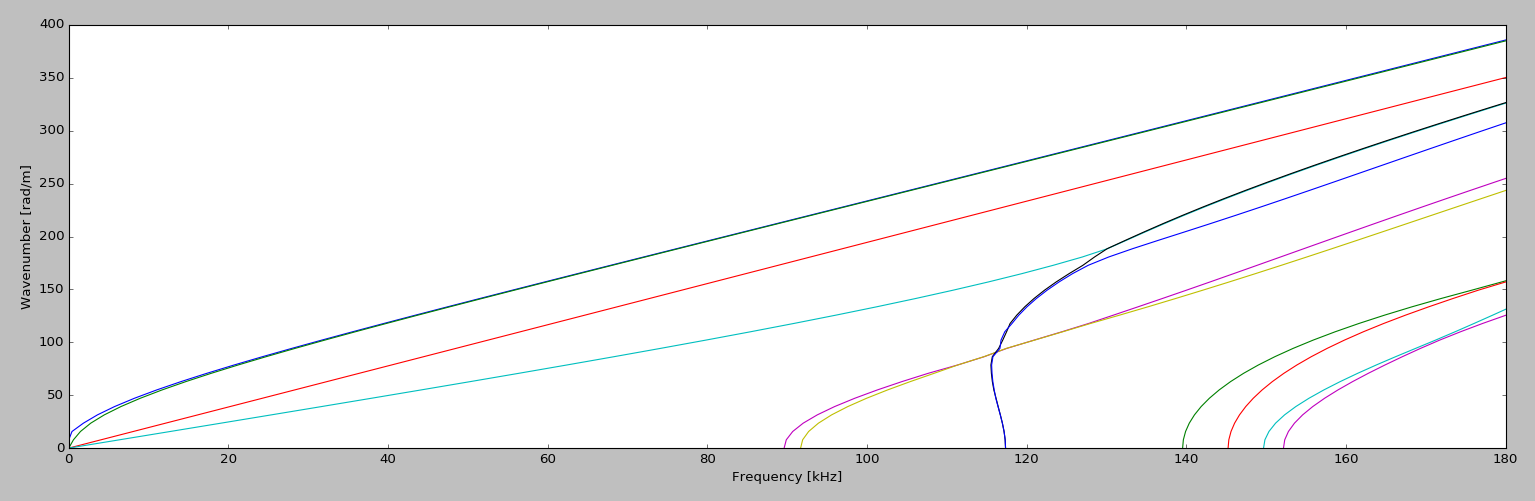
\includegraphics[width=13cm]{Zdjecia/4/zagregowane_krzywe}
\caption{Krzywe dyspersji po agregacji}
\label{fig:krzywe_po_agregacji}
\end{figure}
\end{enumerate}  

Jak łatwo zauważyć opisany algorytm w sposób efektywny agreguje chmurę punktów do odpowiednich krzywych. Uporządkowoane w ten sposób punkty zostały wykorzystane do opracowania trzech metod kompensacji, opisanych w kolejnych sekcjach tego rozdziału.





\section{Metoda odwracania sygnału w czasie}
\label{sec:metoda_tr}

Metoda omawiana w tej sekcji polega na wygenerowaniu sygnału który po przepropagowaniu pewnej odległości sam się skompensuje. Technika kompensacji dyspersji poprzez wygenerowanie sygnału odwróconego w czasie została zaprezentowana w artykule \cite{kasia4}

\subsection{Podstawy teoretyczne}
Podstawową ideą prezentowanej w tej części pracy techniki kompensacji dyspersji jest wytworzenie sygnału, który poprzez nałożenie składowych częstotliwości w czasie propagacji skompensuje się, tworząc oczekiwany sygnał w pozycji pomiarowej. W przypadku w którym do obiektu wprowadzony zostanie zwykły sygnał sinusoidalny o liniowo zmieniającej się częstotliwości (linear-chirp) zostanie wzbudzone przynajmniej kilka trybów fali prowadzonej. Każdy tryb w każdej z częstotliwości może poruszać się z różną prędkością fazową i grupową. Ze względu na dyspersję sygnał wraz z propagacją będzie stawał się coraz dłuższy a jego amplituda będzie spadać, ponieważ ulegnie on rozproszeniu.  Składowe częstotliwości sygnału odpowiadające najwyższym prędkością grupowym będą znajdować się z przodu, natomiast wolniejsze komponenty będą znajdowały się z tyłu. Podstawa przedstawianej metody polega na założeniu, że tak otrzymany sygnał jesteśmy w stanie odwrócić w czasie, tak aby komponenty o mniejszej prędkości znalazły się z przodu sygnału a komponenty o większej prędkości znalazły się z tyłu. Wzbudzenie obiektu tak przygotowanym sygnałem da w odpowiedzi sygnał skompensowany tej samej postaci co pierwotne wzbudzenie. Skuteczność metody można wykazać analitycznie. Przyjijmy, że sygnał zastosowany do wzbudzenia pręta zostanie zastosowany w punkcie $x = 0$ i będzie to sygnał $f(t)$. Sygnał wzbudzający w dziedzinie częstotliwości możemy zapisać jako:
\begin{equation}
[F(\omega)_{x=0}]=\int\limits_{-\infty}^{\infty}f(t)e^{-i\omega t}dt \label{eq:F(omega)_x=0}
\end{equation}
Jeśli przez nasz obiekt propaguje jedna postać fali to w punkcie $x=L$ można tę funkcję zapisać jako:

\begin{equation}
[F(\omega)_{x=L}]=\int\limits_{-\infty}^{\infty}f(t)e^{-i(\omega t - kL}dt \label{eq:F(omega)_x=L}
\end{equation}

gdzie liczba falowa k jest funkcją częstotliwości $\omega$  , która jest opisana za pomocą krzywej dyspersji dla danego trybu fali. Równania (\ref{eq:F(omega)_x=0}) oraz (\ref{eq:F(omega)_x=L}) można powiązać funkcją przejścia $H(\omega)$ co można zapisać jako:
\begin{equation}
H(\omega) = \frac{[F(\omega)]_{x=L}}{[F(\omega)]_{x=0}} \label{eq:h(omega)}
\end{equation}

Zakładając, że chcemy uzyskać sygnał $g(t)$, którego transformata Fouriera to $G(\omega)$ przy ($x = L$) wtedy wymagany sygnał wejściowy ($x = 0$) $Y(\omega)$:
\begin{equation}
Y(\omega) = \frac{G(\omega)}{H(\omega)} = G(\omega)[H(\omega)]^{-1} \label{eq:Y(omega)}
\end{equation}
Sygnał w dziedzinie czasu y(t) jaki musi zostać wprowadzony do badanego pręta w punkcie $x=0$ aby uzyskać odebrany sygnał $g(t)$ w punkcie $x=L$ można uzyskać z odwrotnej transformaty Fouriera, co pokazuje równanie (\ref{eq:Y(omega)}):
\begin{equation}
y(t) = \frac{1}{2\pi}\int\limits_{-\infty}^{\infty}\frac{G(\omega)}{H(\omega)}e^{i\omega t}d\omega \label{eq:y(t)}
\end{equation}

W prostym przypadku gdy analizujemy pojedynczą postać fali prowadzonej:
\begin{equation}
[H(\omega)]^{-1} = e^{-ikL} = e^{-i\omega L/c}
\end{equation}
\begin{equation}
y(t) = \frac{1}{2\pi}\int\limits_{-\infty}^{\infty}G(\omega)e^{-i\omega (L/c - t)}d\omega
\end{equation}

Przyjmując, że sygnał w domenie czas $g(t)$ jest aplikowany w punkcie $x = 0$ sygnał $y^*(t)$ w punkcie x = L można zapisać jako:
\begin{equation}
y^*(t) = \frac{1}{2\pi}\int\limits_{-\infty}^{\infty}G(\omega)e^{-i\omega (L/c + t)}d\omega
\end{equation}

Technika kompensacji w tym przypadku polega na odebraniu sygnału $y^*(t)$ w przedziale czasowym $t\in [0,T]$ w którym cała paczka falowa zostanie odebrana przez odbiornik. Następnie sygnał zostaje odwrócony w czasie. Otrzymany w ten sposób sygnał może być zaaplikowany do badanego pręta. W trakcie propagacji zostanie on skompensowany do fali o kształcie takim jak kształt sygnału $g(t)$

\subsection{Implementacja numeryczna}
W ramach niniejszej pracy, omawiana metoda została zaimplementowana do aplikacji. Podstawa jej działania opiera się na znajomości krzywych dyspersji. Pierwszym etapem jest wygenerowanie sygnału, jaki chce się uzyskać w wyniku kompensacji. Następnie dzięki zaimplementowanym metodom należy uzyskać przewidywany kształt sygnału po przepropagowaniu zadanej odległości oraz odrócenie go w czasie. Sygnał otrzymany z tak przygotowanego sygnału wejściowego powinien skompensować się na zadanej odległości. Rysunek \ref{fig:kolejne_etapy_TR} przedstawia opisane kroki na przykładzie sygnału linear chirp.
\begin{figure}[h]
\centering
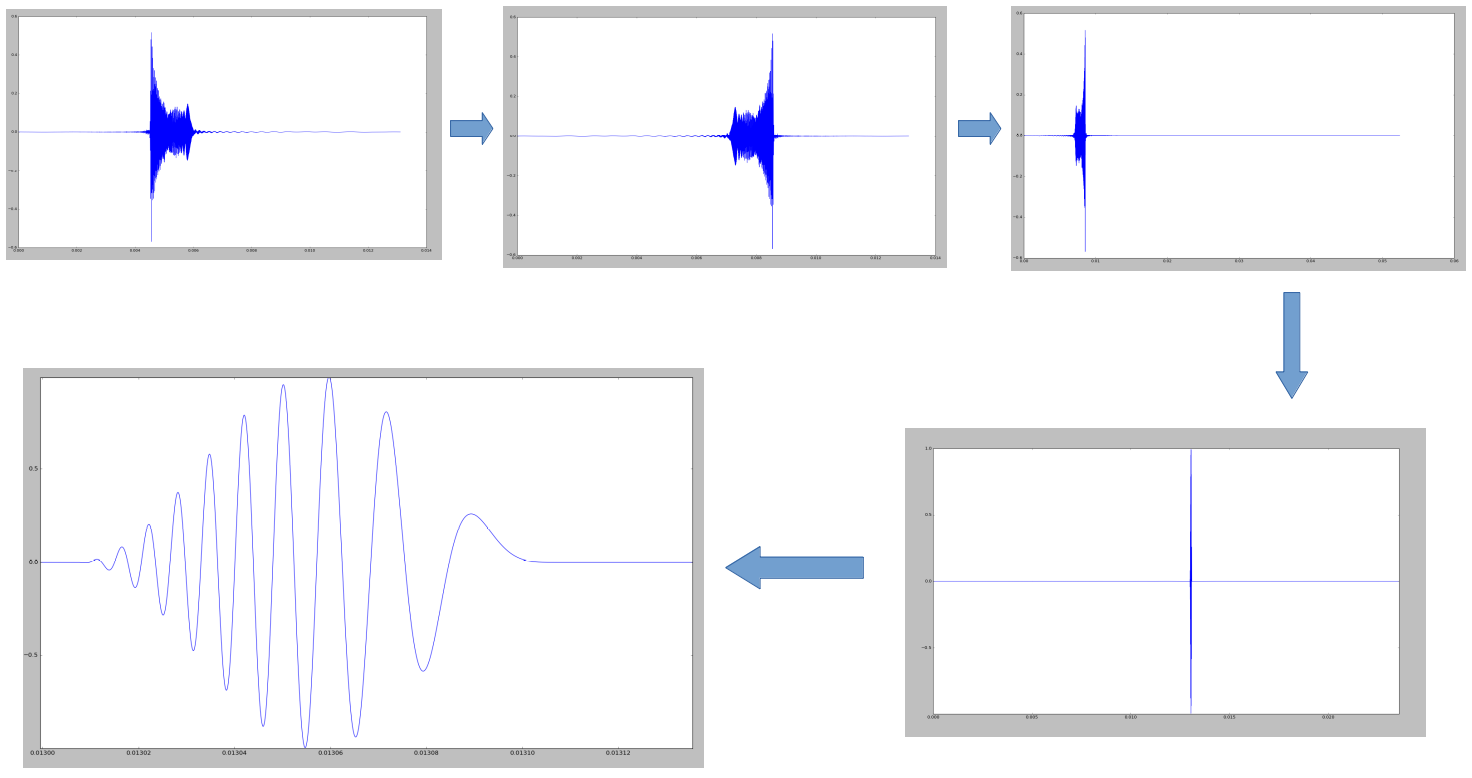
\includegraphics[width=14cm]{Zdjecia/4/algorytm_komp_tr}
\caption{Algorytm kompensacji odwracania czasu}
\label{fig:kolejne_etapy_TR}
\end{figure}

W zaprezentowanym przykładzie odwrócony w czasie sygnał został dodatkowo wypełniony zerami. Zabieg ten został zastosowany, ponieważ całość została przeprowadzona w ramach symulacji i wypełnienie sygnału było konieczne do przeprowadzenia prawidłowej symulacji propagacji. Przedstawiana metoda pozwala zatem wygenerować sygnał kompensujący się na zadanej odległości do fali o oczekiwanym kształcie. Pozwala na propagowanie zarówno pojedynczego trybu jaki nałożonych wielu postaci fali prowadzonej. Jednak aby móc stosować tę motodę konieczna jest znajomość długości ścieżki propagacji sygnału. Jeżeli ściażka propagacji ulegnie zmianie, konieczne jest wygenerowanie nowego sygnału adekwatnego do aktualnego badanego obiektu. W przypadku w którym podczas propagacji następowałyby dodatkowe odbicia, na przykład w sytuacji, w której fala propagujące przez dwa pręty złączone ze sobą, część energii zostanie odbita od punktu złączenia a część przepropaguje przez drugi pręt i odbije się na końcu. Stworzenie sygnału kompensującego się w takiej sytuacji byłoby bardziej skomplikowane i nie zostało opisane w tej pracy. Rysunek \ref{fig:rozne_odl} prezentuje przykład fali przygotowanej do kompensacji po 4 metrach propagacji, który przepropagował kolejno 1,2,4 i 5 metrów.

\begin{figure}[h]
\centering
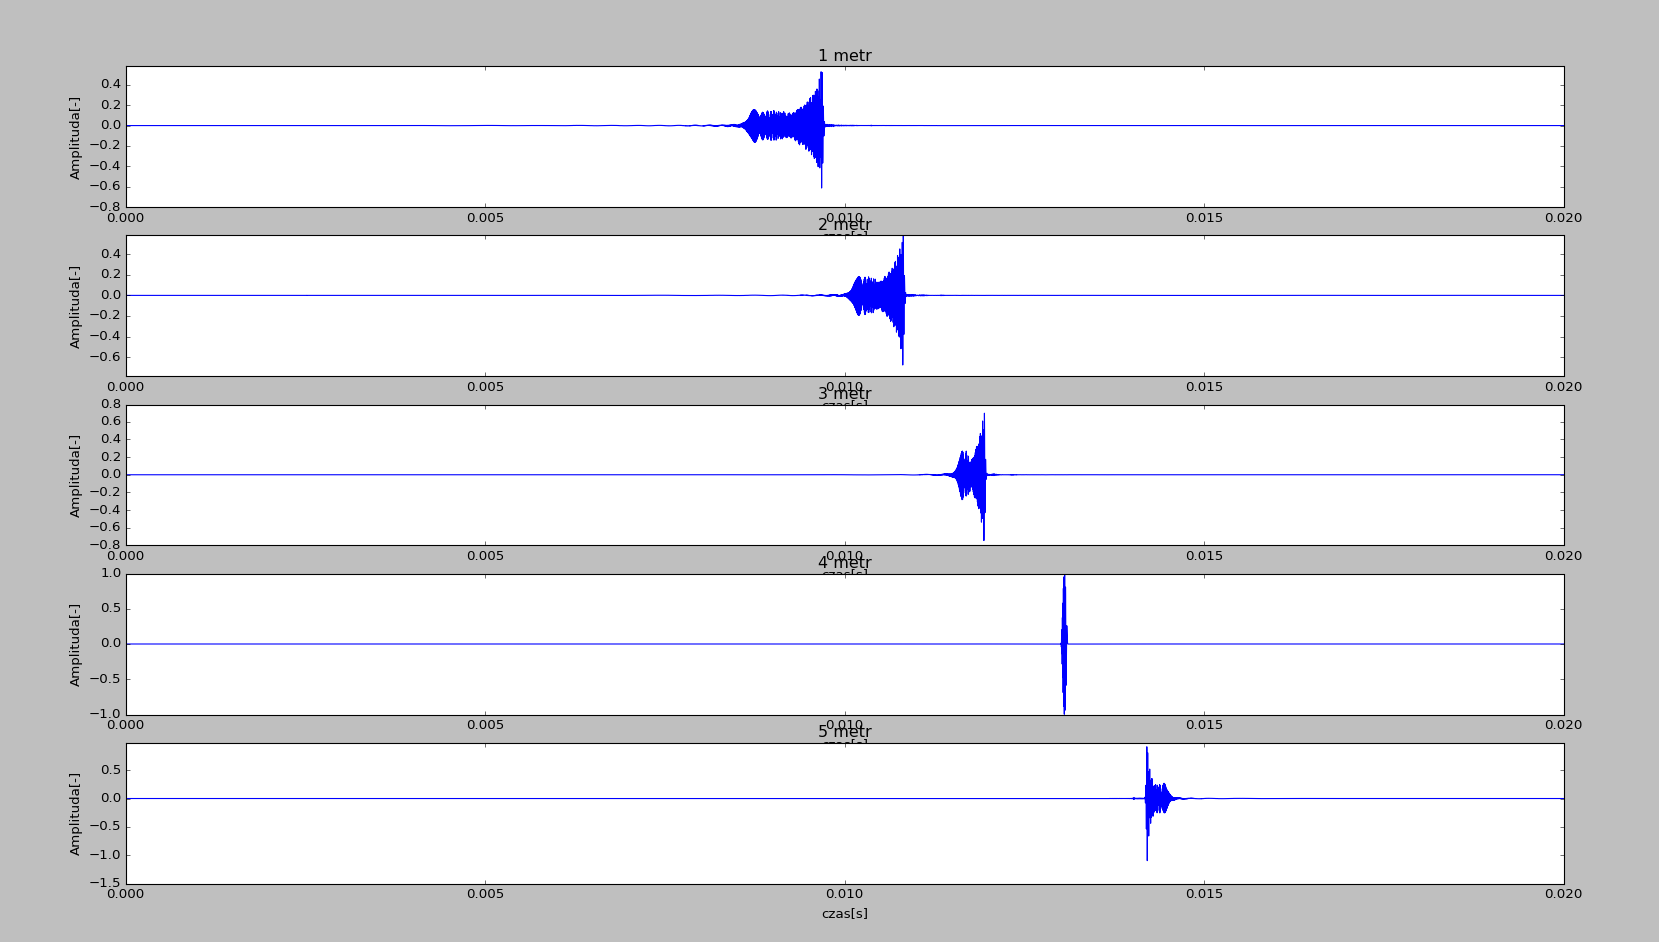
\includegraphics[width=14cm]{Zdjecia/4/porownanie_roznych_odleglosci_time_reversal}
\caption{Sygnał przygotowany do kompensacji po 4 metrach propagacji przedstawiony kolejno po 1, 2, 4 i 5 metrach propagacji}
\label{fig:rozne_odl}
\end{figure}

Jak łatwo zauważyć wprowadzony sygnał kompensuje się tylko i wyłącznie po przepropagowaniu założonej odległości. wraz z oddalaniem się od punktu, w którm przewidziany był odbiornik efekt dyspersji się nasila. Tak więc zarówno przed jak i za założonym punktem odbioru odebrany sygnał byłby rozproszony. Metoda ta może służyć do przeprowadzania nieniszczących testów obiektów o znanej charakterystyce przejścia. W sytuacji w której w strukturze nie będzie żadnych uszkodzeń otrzymywany sygnał będzie skompensowany. Natomiast gdy pojawią się uszkodzenia, nieciągłości w strukturze spowodują odbicie fali i skrócenie ścieżki propagacji co da informację o uszkodzeniach. 

\subsection{Wybrane wyniki z symulacji}
Rysunek \ref{fig:sygnal we} przedstawia sygnał przekazany do funkcji, jako ten, do którego sygnał ma się skompensować po przepropagowaniu zadanej odległości
\begin{figure}[h]
\centering
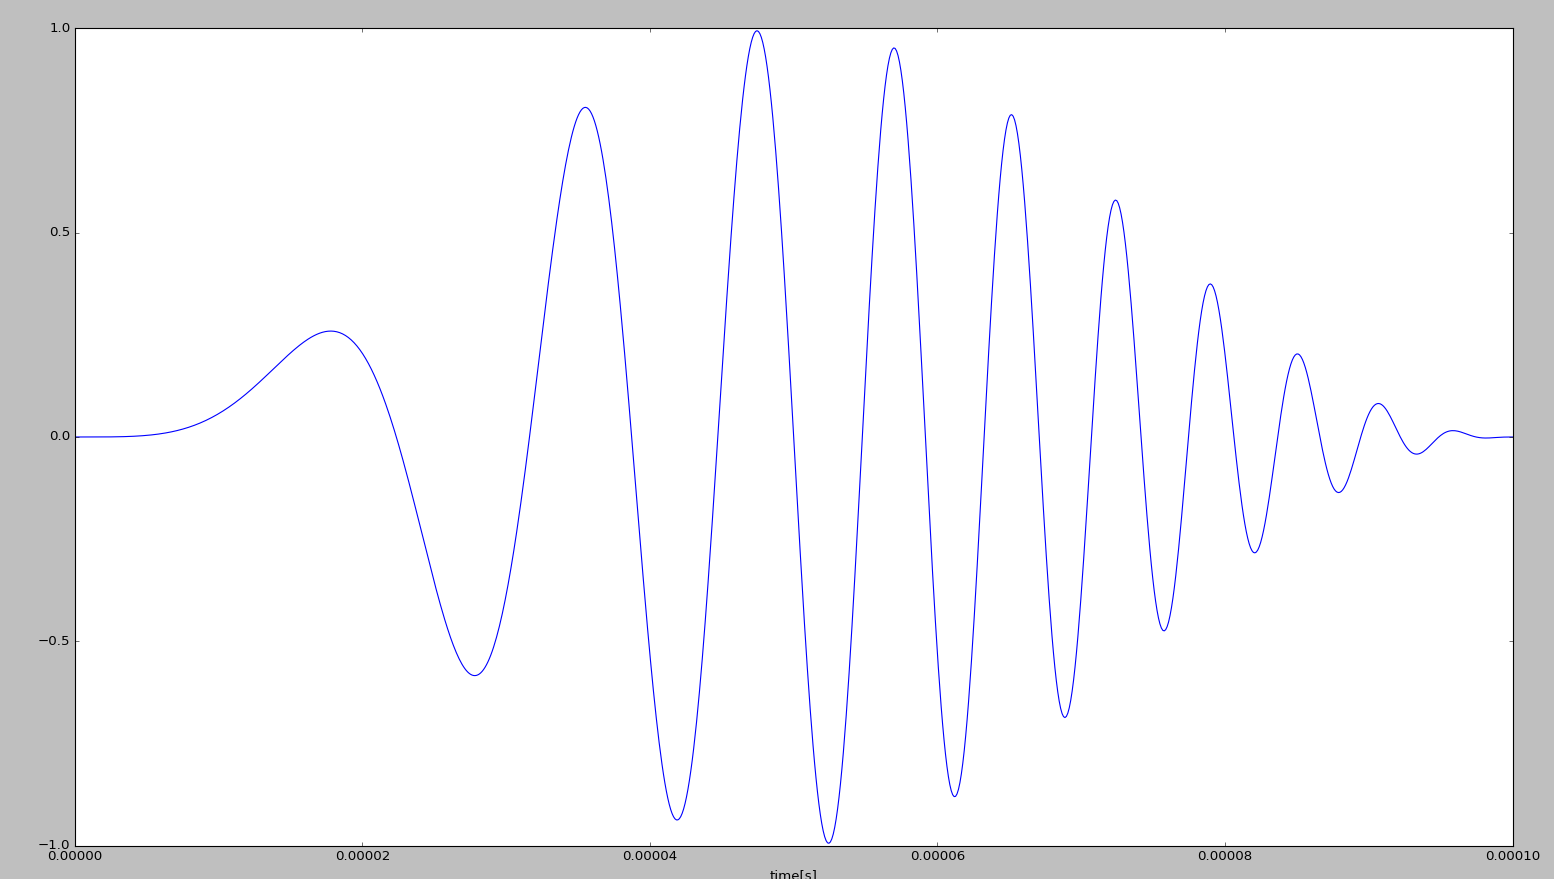
\includegraphics[width=14cm]{Zdjecia/4/test_chirp}
\caption{Algorytm kompensacji odwracania czasu}
\label{fig:sygnal we}
\end{figure}
Wygenerowany przez aplikację sygnał jest różny dla różnych zadanych odległości. Obrazuje to rysunek \ref{fig:rozne_odl} na którym przedstawiono sygnały mające się skompensować odpowiednio po 1, 2, 3, 4 metrach, gdy propagują pierwsze cztery postaci fali prowadzonej. 
\begin{figure}[h]
\centering
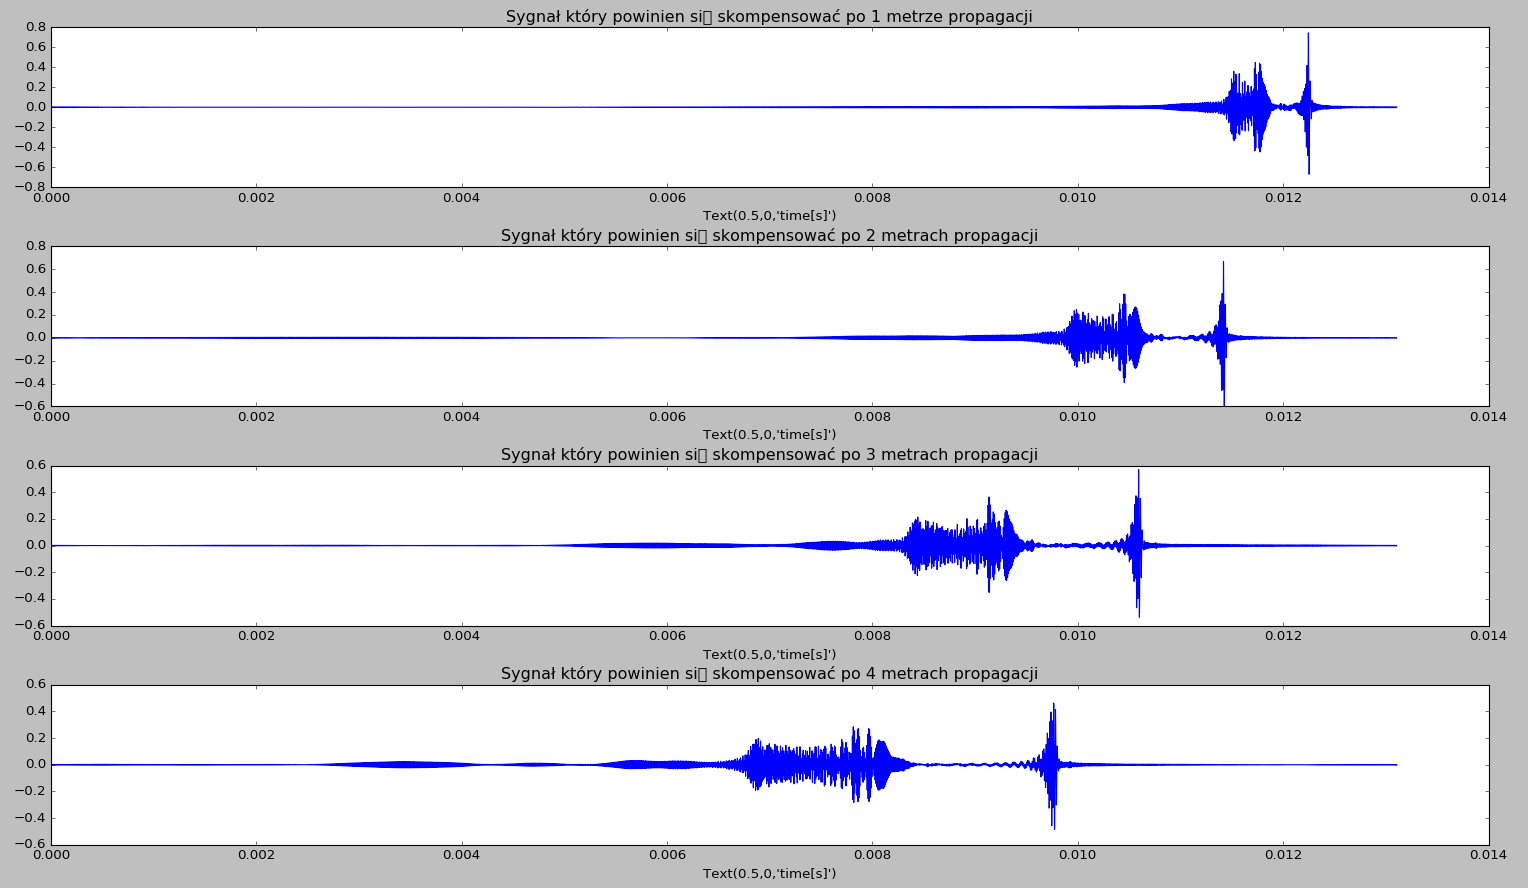
\includegraphics[width=14cm]{Zdjecia/4/tr_przykl}
\caption{Sygnał przygotowany do kompensacji po odpowiedno 1,2,3 oraz 4 metrach}
\label{fig:rozne_odl}
\end{figure}
Sygnał jest też różny dla różnej ilości propagujących trybów, rysunek \ref{fig:rozne_tryby}. Jak łatwo zauważyć, im większa ilość propagujących postaci tym bardziej widoczne staje się zjawisko dyspersji i tym dłuższy staje się przepropagowany sygnał.
\begin{figure}[h]
\centering
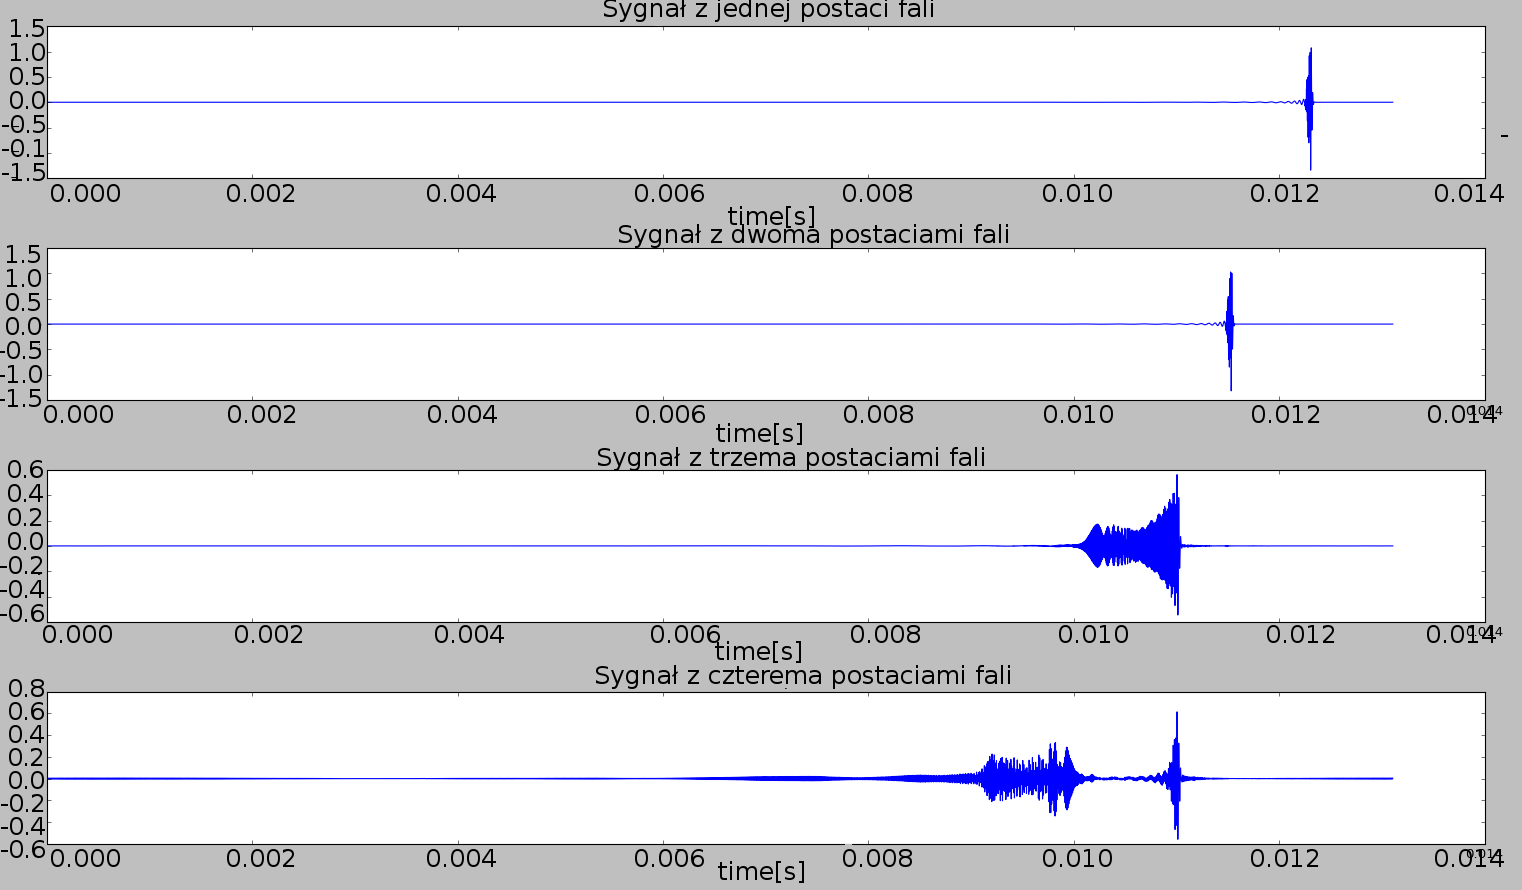
\includegraphics[width=14cm]{Zdjecia/4/TR-rozna_ilosc_modow}
\caption{Sygnał przygotowany do kompensacji po 2,5 metra propagacji zawierający kolejno 1,2,3 oraz 4 postaci fali prowadzonej}
\label{fig:rozne_tryby}
\end{figure}
Tak wygenerowane sygnały zostały przetestowane przez propagację w symulacji. Rysunek \ref{fig:100} ilustruje jak ważna jest znajomość długości ścieżki propagacji. Jeśli sygnał przebędzie zbyt krótką lub zbyt długą drogę to odebrany sygnał nie będzie skompensowany.
\begin{figure}[h]
\centering
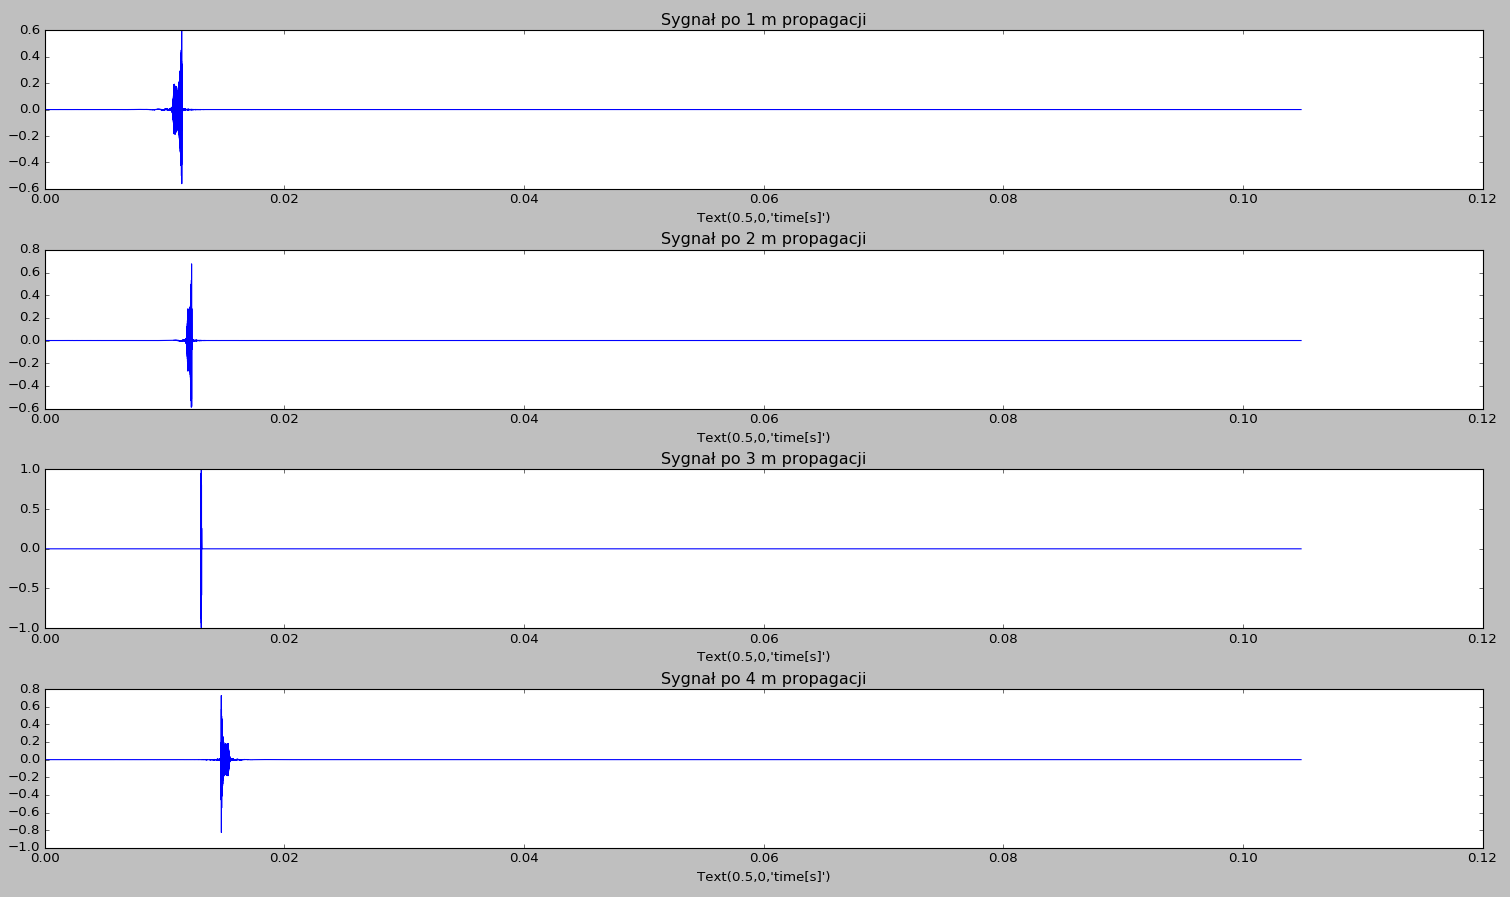
\includegraphics[width=14cm]{Zdjecia/4/obrazek100}
\caption{Sygnał przygotowany do kompensacji po 3 metrach propagacji przepropagowany kolejno o 1,2,3 i 5 metrów}
\label{fig:100}
\end{figure}
Rysunek \ref{fig:skompensowane_TR} ilustruje wyniki symulacji propagacji na odpowiednie odległości sygnałów przedstawinych na rysunku 4.9
\begin{figure}[h]
\centering
\includegraphics[width=14cm]{Zdjecia/4/skompensowane_TR}
\caption{Sygnały  z rysunu 4.9 po przepropagowaniu odpowiednich odległości}
\label{fig:skompensowane_TR}
\end{figure}

Rysunek \ref{fig:tr_rozna_il_postaci_skomp} ilustruje wyniki  symulacji propagacji sygnałów przedstawionych na rysunku 4.10. Łatwo zauważyć, że wyniki symulacji dają bardzo dobre rezultaty. 
\begin{figure}[h]
\centering
\includegraphics[width=14cm]{Zdjecia/4/tr_rozna_il_postaci_skomp}
\caption{Sygnały  z rysunu 4.10 po przepropagowaniu odpowiedniej odległości}
\label{fig:tr_rozna_il_postaci_skomp}
\end{figure} 

Rysunek \ref{fig:porownanie} przedstawia porównanie wyniku symulacji sygnału linear chirp po propagacji dwóch metrów w pręcie w którym propagowały trzy pierwsze tryby fali prowadzonej (kolor niebieski) oraz sygnału wygenerowanego w aplikacji, przygotowanego do kompensacji po dwóch metrach. Łatwo zauważyć, że przedstawiana metoda pozwala znacząco skrócić czas trwania odbieranego sygnału. Sygnał bez kompensacji trwa 6e-4s natomiast z 1e-4 czyli dokładnie tyle ile żądany sygnał. A zatem można stwierdzić iż kompensacja została skutecznie przeprowadzona. Kolejny rysunek przedstawia porównanie sygnału założonego na wejściu, jako jako postać do której powinien on zostać skompensowany, oraz sygnału faktycznie otrzymanego po symulacji propagacji. Czas trwania oraz obwiednia sygnału zgadzają się z założeniami, jednak widać iż otrzymany sygnał jest sygnałem odwróconym w czasie w stosunku do założonego sygnału. Wynik nie jest zatem idealnym odwzorowaniem założeń, niemniej jednak otrzymany sygnał został maksymalnie skompensowany. W otrzymanym sygnale nie ma również widocznych szumów, pogarszających czytelność otrzymanego wyniku. Oczywistym jest fakt, iż w przypadku rzeczywistym szumy z pewnością by występowały. Idealne matematyczne odwzorowanie padanego obiektu nie jest możliwe, lecz mimo to metoda powinna dawać dobre rezultaty.

\begin{figure}[h]
\centering
\includegraphics[width=14cm]{Zdjecia/4/tr_porownanie}
\caption{Porównanie sygnału bez kompensacji(górny) oraz z kompensacją (dolny)}
\label{fig:porownanie}
\end{figure} 

\begin{figure}[h]
\centering
\includegraphics[width=14cm]{Zdjecia/4/tr_porownanie2}
\caption{Porównanie sygnału oczekiwanego(górny) otrzymanego (dolny)}
\label{fig:porownanie2}
\end{figure} 


\section{Metoda mapowania liniowego przy pomocy rozwinięcia w szereg Taylora}
\label{sec:Taylor}
Prezentowana w poniższej sekcji metoda kompensacji dyspersji została przedstawiona w artykule []\textcolor{red}{referenacja do yuanliu}
\subsection{Podstawy teoretyczne}
Po wzbudzeniu badanego pręta odpowiednim sygnałem wejściowym, możliwe jest aby przełączył się on w tryb obioru sygnału i nasłuchiwał nadejścia odpowiedzi układu. W takim wypadku odpowiedź jaką uzyskamy będzie sumą odpowiedzi ze wszystkich odbić, od końca pręta oraz ewentualnych łączeń lub uszkodzeń.  Proponowana w tym rozdziale metoda opiera sie na założeniu, że w badanym obiekce propaguje jedna wybrana postać drgań. Jej celem jest kompensacja powstałej dyspersji, tak aby sygnały z różnych punktów odbicia nie nachodziły na siebie i była możliwa ich interpretacja w celu ustalenia ilości punktów odbicia oraz oszacowania ich odegłości od miejsca wzbudzenia na podstawie znajomości prędkości grupowej fali. Przy tak sformułowanych założeniach, sygnał otrzymany w odbiorniku można przedstawić wzorem:
\begin{equation}
g(t) = \sum\limits_{n=1}{N}f_n(r_n,t)=\frac{1}{2\pi}\int _{-\infty}^{\infty}F(\omega)\sum\limits_{n=1}^{N}(A_n(\omega)e^{-ikr_n})e^{i\omega t} d\omega \label{eq:g(t)_taylor}
\end{equation}
Gdzie:

$N$ - całkowita liczba ścieżek propagacji sygnału (liczba punktów odbicia)

$r_n$ - długość n-tej ścieżki propagacji

$A_n$ - współczynnik odbicia n-tego punktu odbicia.

Widmo częstotliwości takiego sygnału $G(\omega)$  możemy obliczyć przy pomocy transformaty Fouriera i zapisać wzorem:
\begin{equation}
G(\omega) = F(\omega)\sum\limits_{n=1}^{N}(A_n(\omega)e^{-ikr_n} \label{eq:G(omega)_taylor}
\end{equation}

Jak wiadomo, dyspersja zależy od kształtu krzywej dyspersji, $k = K(\omega)$. Jeśli więc $K(\omega)$ jest funkcją kwadratową lub wyższego rzędu względem $\omega$, to $G(\omega)$ reprezentuje widmo częstotliwości rozproszonych pakietów fal. Jeśli natomiast zależność $K(\omega)$ byłoby funkcją liniową, zjawisko dyspersji nie występowałoby, a $G(\omega)$ reprezentowałoby widmo częstotliwości sygnału, który nie uległ dyspersji. 
Wybraną krzywą dyspersji można przybliżyć przy pomocy rozwinięcia w szereg Taylora:
\begin{equation}
k = K(\omega) - k_0+k_1(\omega - \omega _0) + k_2(\omega - \omega _0^2)+... \label{eq:szereg_k}
\end{equation}

Gdzie:

$k_0 = \frac{\omega _0}{c_p}$

$k_1 = \frac{dk}{d\omega}|_{\omega = \omega_0}$

$k_2 = \frac{1}{2}\frac{d^2k}{d\omega ^2}|_{\omega = \omega _0}$

$c_p$ - prędkość fazowa

Wynika z tego, iż dyspersję sygnału można usunąć usuwając jej nieliniowy składnik, poprzez zastąpienie oryginalnej zależności $K(\omega)$ liniowym przybliżeniem tej funkcji. Zastosowanie takiego zabiegu sprawi, iż sygnał w dziedzinie czasu będzie postrzegany jako skompensowany do postaci niedyspersyjnej, a prędkość grupowa obliczona z liniowego przybliżenia krzywej dyspersji może zostać wykorzystana do określenia długości ścieżek propagacji wynikających z kolejnych odbić. 

W szczególnym przypadku, w którym mamy do czynienia z pojedyńczą ścieżką propagacji ($N=1$) i odległość między nadajnikiem a punktem odbicia jest znana, można usunąć dyspersję poprzez wyeliminowanie wyrażenia kwadratowego w $K(\omega)$. Matematycznie można to zrobić przy pomocy wzoru:
\begin{equation}
 \widetilde{G}(\omega)=(F(\omega)A_1(\omega)e^{-ikr_1})e^{ik_2(\omega -\omega _0)^2r_1}
\end{equation}

Gdzie $\widetilde{G}(\omega)$ jest zmodyfikowanym widmem częstotliwości, a $r_1$ jest odległością między nadajnikiem i odbiornikiem. Sygnał skompensowany w dziedzinie czasu można natychmiast uzyskać poprzez odwrotną transformatę Fouriera. Ponieważ jednak zazwyczaj długość ścieżki propagacji sygnału nie jest znana, a sygnał może składać się z wielu odbić, między innymi od uszkodzeń ($N>1$) usuwanie dyspersji przy pomocy powyższego wzoru byłoby niepraktyczne. 

Rysunek \ref{fig:krzywa_taylorem} obrazuje przykład krzywej dyspersji, trybu $A_0$, płyty aluminiowej o grubości 3,175 mm. Linia ciągła pokazuje zależności $K(\omega)$ uzyskaną metodami komputerowymi, natomiast linia przerywana kropkowana wskazuje z rozwinięcie szeregu Taylora pierwszego rzędu, a linia przerywana rozszerzenie szeregu Taylora drugiego rzędu w odniesieniu do centralnej częsości kątowej ($\omega _0 = 2\pi *50 kHz$)

\begin{figure}[h]
\centering
\includegraphics[width=14cm]{Zdjecia/4/buba}
\caption{Przykładowe porównanie oryginalnej krzywej oraz jej przybliżeń przy pomocy rozwinięcia w szereg Taylora}
\label{fig:krzywa_taylorem}
\end{figure}

Łatwo zauważyć, że po pierwsze, rozszerzenie drugiego rzędu daje bardzo dobrze przybliżenie pierwotnego kształtu krzywej, po drugie, $K(\omega)$ jest monotoniczną funkcją $\omega$ w otoczeniu $\omega _0$. 

Równanie \ref{eq:G(omega)_taylor} można zapisać w postacji złożenia funkcji:
\begin{equation}
G(\omega) = G(k)\circ K(\omega)
\end{equation}

Gdzie $\circ$ jest operatorem składania funkcji. $G(k)$ jest niejawną funkcją k z równania \ref{eq:G(omega)_taylor}. Zamieniając $K(\omega)$ na $K_{lin}(\omega)$ będące aproksymacją $K(\omega)$ pierwszego rzędu w punkcie $\omega _0$, gdzie $\omega _0$ oznacza częstotliwość o najwyższej energii, można wyprowadzić zmodyfikowane widmo częstotliwości:
\begin{equation}
\widetilde{G}(\omega) = G(k)\circ K_{lin}(\omega)
\end{equation}

Ponieważ $G(\omega)$ jest znane oraz znana jest analizowana krzywa dyspersji, znane jest również $G(k)$, obliczając przybliżenie liniowe $K_{lin}(\omega)$ można w prosty psosób obliczyć $\widetilde{G}(\omega)$, poprzez interpolację odpowiednich wartości. Opisana metoda może być określana mianem mapowania liniowego. W jej efekcie uzyskane zostaje nowe widmo częstotliwości $\widetilde{G}(\omega)$. Po mapowaniu widmo amplitudy pozostaje bez zmian, natomiast widmo fazy stopniowo odbiega od pierwotnego w miarę oddalania się od wybranej, środkowej częstotliwości, co dobrze ilustruje rysynek \ref{fig:widma}

\begin{figure}[h]
\centering
\includegraphics[width=14cm]{Zdjecia/4/widma}
\caption{Przykładowe porównanie oryginalnych charakterystyk oraz ich przybliżeń przy pomocy rozwinięcia w szereg Taylora}
\label{fig:widma}
\end{figure}

Należy zaznaczyć, iż stosowanie omawianej metody jest możliwe tylko w sytuacji, gdy $K(\omega)$ jest funkcją monotoniczną

\subsection{Implementacja numeryczna}
Implementacja prezentowanej metody opiera się głównie na znajomości krzywej dyspersji, której propagację bierzemy pod uwagę. Pierwszym krokiem, jest wygenerowanie odpowiedniego sygnału testowego. Mając właściwy sygnał można przystąpić do właściwego procesu kompensacji. W pierwszej kolejności analizowane jest widmo amplitudowe otrzymanego sygnału. Na jego podstawie uzyskiwana jest informacja o częstotliwości z największą energią. Zostaje ona wybrana na częstotliwość w której nastąpi przybliżenie liniowe. Po wybraniu $\omega _0$ odnajdywane jest na krzywej dyspersji odpowiednia wartość liczby falowej. Korzystając z zależności opisujących wartości $k_0$ i $k_1$ wyliczone zostaje liniowe przybliżenie badanej krzywej. Uzyskane w aplikacji wyniki przedstawia rysunek \ref{fig:krzywa_moja}. Linia niebieska prezentuje oryginalną krzywą dyspersji, natomiast linia zielona przdstawia jej przybliżenie uzyskane w aplikacji przy użyciu rozwinięcia w szereg Taylora.

\begin{figure}[h]
\centering
\includegraphics[width=14cm]{Zdjecia/4/krzywa_moja}
\caption{Przykładowe porównanie oryginalnej krzywej oraz jej przybliżeń przy pomocy rozwinięcia w szereg Taylora}
\label{fig:krzywa_moja}
\end{figure}

Kolejnym krokiem implementowanego algorytmu, jest wyliczenie G(k) na podstawie otrzymanego widma sygnału $G(\omega)$ na podstawie krzywej dyspersji. Następnie ponowne wyznaczenie zależności w dziedzinie częstotliwości, tym razem jednak używając przybliżenia liniowego zamiast oryginalnej krzywej dyspersji. Omawiany algorytm doskonale ilustruje rysunek \ref{fig:algo_Taylora}

\begin{figure}[h]
\centering
\includegraphics[width=13cm]{Zdjecia/4/algo_Taylora}
\caption{Wizualizacja algorytmu []Przypis do Pialucha}
\label{fig:algo_Taylora}
\end{figure}

Przedstawia on krzywą $G(\omega)$ z aż trzema osiami poziomymi. Linia ciągła przedstawia zależność $G(K(\omega))$, czerwonymi kółkami oznaczony jest sygnał $G(\omega)$. Jak widać przejście z dziedziny $K(\omega)$ na $\omega$ jest nieliniowe co wynika z niliniowego charakteru krzywej dyspersji. Zielonymi trójkątami oznaczono natomiast krzywą $G(K_{lin}(\omega))$. Jak widać przejście z dziedziny $\omega$ na $K_{lin}(\omega)$ jest przejściem o charakterze liniowym. 
\subsection{Wybrane wyniki symulacji}
Rysunek \ref{fig:liniakrzyws} obrazuje przybliżenie krzywej dyspersji wyznaczonej dla zadanego sygnału z rysunku 4.8.
\begin{figure}[h]
\centering
\includegraphics[width=13cm]{Zdjecia/4/krzywa_moja}
\caption{Porównanie oryginalnej krzwej z jej liniowym przybliżeniem}
\label{fig:liniakrzyws}
\end{figure}
Rysunek \ref{fig:przedipo} ilustruje przykład sygnału przed i po kompensacji.
\begin{figure}[h]
\centering
\includegraphics[width=13cm]{Zdjecia/4/przedipo}
\caption{Porównanie sygału przed i po kompensacji}
\label{fig:przedipo}
\end{figure}
Na ostatnim rysunku przedstawione zostało porównanie otrzymanych w wyniku kompensacji sygnałów z sygnałem zadanym \ref{fig:przedipo2}
\begin{figure}[h]
\centering
\includegraphics[width=13cm]{Zdjecia/4/przedipo2}
\caption{Porównanie sygnału oryginalnego z sygnałem skompensowanym}
\label{fig:przedipo2}
\end{figure}

\section{Metoda mapowania sygnału z dziedziny czasu na dziedzinę odległości}
\label{sec:Wilcox}

Opisana w poniższej sekcji metoda została zaprezentowana w artykule \cite{kasia1}. Opiera się na odpowiednim zastosowaniu transformaty Fouriera. Pozwala na kompensację sygnału poprzez przejście z dziedziny czasu na dziedzinę odległości, dzięki czemu w wyniku otrzymywany jest skompensowany sygnał oraz informacja o długości ścieżki propagacji.

\subsection{Podstawy teoretyczne}

W niniejszej pracy rozważaną strukturą, w której powstają i propagują fale prowadzone jest długi stalowy pret. Przyjmując oznaczenie sygnału wejściowego jako $f(t)$, natomiast propagujący w pręcie sygnał jako $u(x,t)$ zakłada się iż w miejscu wzbudzenia, zachodzi zależność: 
\begin{equation}
u(x,t) = f(t)
\end{equation}
Znając $u(x,t)$ w jednym punkcie w przestrzeni oraz znając charakterystykę propagującego trybu lub trybów fali prowadzonej, można odtworzyć sygnał po dowolnej odległości propagacji oraz w dowolnym punkcie czasowym. Można to osiągnąć rozważając przesunięcie fazowe każdej składowej częstotliwości oddzielnie:
\begin{equation}
u(x,t) = \int\limits_{-\infty}^{\infty}F(\omega)e^{i(k(\omega)x - \omega t)}d\omega \label{eq:propagacja_jeden_mod}
\end{equation}
Propagacja więcej niż jednego trybu fali oznacza, iż dana częstotliwość wzbudziła więcej niż jedną jej postać. Co za tym idzie w takim przypadku również możliwe jest odtworzenie przebiegu fali poprzez lekką modyfikację wzoru \ref{eq:propagacja_jeden_mod}
\begin{equation}
u(x,t) = \int\limits_{-\infty}^{\infty}F(\omega)e^{ -i \omega t}\sum \limits _{j=1}^{n}e^{ik_j(\omega)x} d\omega\label{eq:propagacja_kilka_mod}
\end{equation}
gdzie:

$F(\omega)$ - transforamta Fouriera sygnału $f(t)$

$k_j(omega)$ - wartość j-tej liczby falowej odpowiadającej częstotliwości $\omega$

Jak już zostało wspomniane, otrzymany sygnał g(t) można odwzorować na funkcję odległości bez stosowania algorytmu komepnsacji jedynie poprzez proste odwzorowanie:
\begin{equation}
x=v_{gr}t \label{eq:x=vgrt}
\end{equation}

Gdzie $v_{gr}$ jest prędkością grupową trybu fali prowadzonej, mierzoną zazwyczaj dla częstotliwości środkowej, lub tej o największej energii. Odwzorowanie takie jest proste do osiągnięcia poprzez zwykłe skalowanie osi czasu g(t) na odległośći propagacji. W przypadku takiego odwzorowania, możliwości wykrycia defektów struktury, znajdujących się w bliskiej odległości od innych cech strukturalnych takich jak na przykład koniec badanego pręta czy punkt łączenia dwóch prętów, zależy od czasu trwania poszczególnych sygnałów. Długie sygnały będą się na siebie nakładać co może doprowadzić do niewykrycia uszkodzenia. Z tego względu sygnał g(t) powinien być jak najkrótszy. 

Przedstawiany algorytm kompensacji dyspersji, zastępuje proste mapowacznie czasu na odległość przy pomocy równania \ref{eq:x=vgrt} takim, które jest wykonywane w domenie liczby falowej. Takie podejście pozwala wziąć pod uwagę prędkości zależne od częstotliwości, czyli wzięcie pod uwagę dyspersji. Niezbędnym elementem omawianej metody jest znajomość krzywych dyspresji badanego obiektu, w zakresie propagowanych trybów. Dokładność z jaką wyliczone krzywe reprezentują rzeczywistą charakterystykę układu, znajduje odzwierciedlenie w jakości uzyskanych wyników. W sytuacji idelanej przedstawiany algorytm przywraca każdy sygnał do dokładnego kształtu pierwotnego, niezależnie od jego odległości propagacji.  

Celem omawianej metody jest przekształcenie otrzymanego sygnału $g(t)$ w funkcję odległości propagacji a nie czasu, oraz skompensowanie rozproszenia otrzymanego sygnału. Dalsze propagowanie otrzymanego sygnału zarówno w przód jak i w tył można otrzymać stosując wzór \ref{eq:propagacja_jeden_mod} lub \ref{eq:propagacja_kilka_mod}. Gdyby obliczyć kompletną mapę odległościowo czasową, sygnał propagujący dalej rozpraszałby się coraz mocniej zarówno w czasie jak i przestrzeni. Natomiast sygnał propagujący wstecz zbiegłby się do swojego minimum w pewnym punkcie, a następnie ponownie rozproszył. Minimum jego trwania przypadłoby na chwilę czasową $t=0$. Dobrze ilustruje to rysunek \ref{fig:Wilcox_propaguje}
\begin{figure}[h]
\centering
\includegraphics[width=14cm]{Zdjecia/4/Wilcox_zasada_dzial}
\caption{Zasada działania omawianej techniki kompensacji dyspersji \cite{kasia1}}
\label{fig:Wilcox_propaguje}
\end{figure}
Obliczenie propagowanego wstecz sygnału dla ujemnych wartości $x'$ w $t=0$ daje dokładnie poszukiwane odwzorowanie z czasu na odlgełość propagacji, która jest poszukiwana i która kompensuje rozproszenie odebranych sygnałów. Nowa zmienna propagacji $x'$ może być zdefiniowana jako $x=-x'$. Wynika z tego, iż propagacja wsteczna może zostać opisana wzorem:

\begin{equation}
h(x) = u(-x',0) = \int \limits_{-\infty}^{\infty}G(\omega)e^{-ik(\omega)x}d\omega \label{eq:wsteczna propagacja}
\end{equation}

gdzie:

$G(\omega)$ - transformata Fouriera odebranego sygnału w dziedzinie czasu $g(t)$

$h(x)$ - skompensowany dyspersyjnie przebieg odległości.

Funkja h(x) przedstawiona jest na rysunku \ref{fig:Wilcox_propaguje} (c).

W niniejszej pracy nie został uwzględniony współczynnik odbicia $A_j$. Na potrzeby symulacji przyjęte zostało iż jest on stały, niezależny od czestotliwości i wynosi 1. Gdyby jednak brać go pod uwagę to wzór 4.16 przyjałby postać:
\begin{equation}
g(t) = \sum \limits _{j}\int\limits_{-\infty}^{\infty}A_j(\omega)F(\omega)e^(ik(\omega)x_j-wt)d\omega
\end{equation}

W przyadku stałego współczynnika odbić wszystkie sygnały w h(x) powinny mieć ten sam kształt obwiedni co oryginalny sygnał wejściowy. Gdyby jednak zależał on od częstotliwości , wówczas obwiednia sygnału w h(x) zostanie zniekształcona i na ogół wydłużona. Takie zniekształcenie jest artefaktem charakterystycznym dla danego punktu odbicia fali. Co za tym idzie takie zakłócenie byłoby obserwowane nawet, gdyby zjawisko dyspersji nie występowało. 

\subsection{implementacja numeryczna}
Równanie \ref{eq:wsteczna propagacja} jest podstawowym równaniem omawianej metody. Jest równaniem kompensacji dyspersji dla funkcji ciągłych. W praktyce sygnał g(t) nie jest sygnałem ciągłym a sygnałem dyskretnym, wygenerowanym w aplikacji lub otrzymanym z przetwornika. Na potrzeby tego rozdziału przyjmijmy nastepujące oznaczenia:

$m$ - liczna próbek sygnału g(t)

$\Delta t$ - okres próbkowania sygnało g(t)

$m\Delta t$ - całkowity czas trwania sygnału g(t)

$n$ - liczba próbek otrzymanego sygnału w dziedzinie odległośći h(x)

$\Delta x$ -przestrzenny okres próbkowania h(x)

$n\Delta x$ - całkowita przestrzenna długość sygnału

Najprostszą implementacją omawianego algorytmu jest poddanie sygnału g(t) szybkiej transformacie Fouriera, a następnie całkowanie numeryczne w zakresie częstotliwości sygnału wejściowego. Takie rozwiązanie byłoby niezwykle czasochłonne ponieważ całkowanie musiałoby zostać wykonane dla każdego z n punkót w skompensowanym sygnale h(x). Metodą, która została zaimplementowana w opisanej aplikacji polega na modyfikacji równania \ref{eq:wsteczna propagacja}. Ta zmiana pozwala na wykonywanie całkowania w ramach algorytmu odwrotnej transformaty Fouriera. Skompensowany sygnał jest funkcją odległości. Odwrotna transformata Fouriera musi zostać zastosowana na sygnale w dziedzinie liczby falowej. Wynika z tego, iż zmienna całkowania w równaniu \ref{eq:wsteczna propagacja} musi zostać zmieniona z $\omega$ na $k$. Można to łatwo zrobić używając poniższych zależności:
\begin{equation}
d\omega = v_{gr}(\omega)dk
\end{equation}
\begin{equation}
\omega = v_{ph}(\omega)k
\end{equation}

Gdzie:

$v_{gr}(\omega)$ - prędkość grupowa propagującej postaci

$v_{ph}(\omega)$ - prędkość fazowa propagującej postaci

Biorąc to pod uwagę równanie \ref{eq:wsteczna propagacja} można zapisać jako:


\begin{equation}
h(x) = \int\limits_{-\infty}^{infty}H(k)e^{-ikx}dk \label{eq:h(x) dobre}
\end{equation}

\begin{equation}
H(k) = G(k)v_gr(k)
\end{equation}

$$
\omega = \omega(k)
$$

Równanie \ref{eq:h(x) dobre} ma postać odwrotnej transformaty Fouriera $H(k)$, w punktach spróbkowanych ze stałym przestrzennym okresem próbkowania $\Delta k$. Uzyskana z transformaty Fouriera funkcja $G(\omega)$ jest funkcją o punktach równomiernie spróbkowanych w dziedzinie częstotliwości. Ze względu na nieliniowy charakter krzywych dyspersji przejście z dziedziny częstości na dziedzinę liczby falowej dałoby w rezultacie funkcję o nierównomiernie spróbkowanej osi k. Aby uzyskać porządany efekt konieczne jest użycie znanej z krzywej dyspersji zależności między wartościami $\omega$ oraz $k$, aby interpolować funkcję G, tak by znaleźć jej wartości w punktach równomiernie rozmieszczonych w dziedzinie liczby falowej.

$G(\omega)$ jest sygnałem zawierającym informacje zarówno o fazie jak i amplitudzie sygnału. W rozwiązaniu numerycznym istotne jest aby dobrać odpowiednie wartości kroków. Zbyt duże ich wartości mogą spowodować utratę informacji, natomiast zbyt małe prowadzą do znacznego wydłużania czasu obliczeń, w zamian za co uzyskiwane wyniki są dokładniejsze i wpływ szumu staje się mniej znaczący. W celu zmniejszenia szumu powodowanego przez błędy interpolacji w końcowym, skompensowanym sygnale, otrzymany sygnał g(t) wypełnia się zerami.W aplikacji użytkownik ma możliwość samodzielnie podać ile razy chce wydłużyć sygnał poprzez wypełnienie zerami. Ograniczenim podlega zarówno $\Delta k$ jak i ilość punktów liczb falowych n. Aby zapobiec zawijaniu sygnału w domenie odległości, minimalna długość skompensowanego sygnału h(x) musi być większa od długości pierwotnego sygnału g(t) pomnożonego przez maksymalną prędkość grupową $v_{max}$.
\begin{equation}
n\Delta x > m\Delta tv_{max}\label{eq:nierownosc dlugosci sygnalow}
\end{equation} 

Powyższa nierówność określa nam maksymalny rozmiar kroku liczby falowej jako:

\begin{equation}
\Delta k = \frac{1}{n\Delta x} < \frac{1}{ m\Delta tv_{max}}\label{eq:nierown delta k}
\end{equation}

Aby cała energia pierwotnego sygnału została poprawnie odwzorowana na dziedzinę odległości, liczba falowa Nyquista $k_{Nyq}$ musi być większa lub równa liczbie falowej trybu fali prowadzonej o częstotliwości Nyquista $f_{Nyq}$ oryginalnego sygnału. Co można zapisać jako:
\begin{equation}
k_{Nyq}\geq k(f_{Nyq})\label{eq:k Nyquista}
\end{equation}
$$
\geq k(\frac{1}{2\Delta t})
$$

Nierówność \ref{eq:k Nyquista} oraz równanie \ref{eq:nierown delta k} pozwalają określić minimalną liczbę punktów w sygnale h(x)
\begin{equation}
n > 2\frac{k_{Nyq}}{\Delta k}
\end{equation}

W zaimplementowanym algorytmie, pierwszym krokiem jest wydłużenie otrzymanego sygnału zadaną ilość razy oraz wykonanie szybkiej transformaty Fouriera na wydłużonym sygnale. Następnie na podstawie przedstawionych ograniczeń dobierana jest wartość kroku $\Delta k$ oraz obliczana wartość $k_{max} = k(\omega _{max})$. Znając te parametry tworzony jest wektor zawierający równomiernie rozłożone wartości liczby falowej. Przy użyciu krzywej dyspersji, interpolując liniowo potrzebne wartości obliczana jest funkcja $G(k)$ oraz $v_{gr}(k)$ w tych samych punktach. Następnie wyliczana zostaje funkcja $H(k)$ mająca równomiernie rozłożone wartości liczby falowej. Ostatnim etapem jest zastosowanie szybkiej odwrotnej transformaty Fouriera co pozwala uzyskać poszukiwany sygnał h(x).

W przypadku gdy mamy do czynienia z propagacją większej ilości postaci fal lub gdy podczas odbicia następuje konwersja trybu fali prowadzonej dokonywane jest uśrednianie propagowanych postaci. Przy założeniu, że propagują jednocześnie dwie postacie równanie \ref{eq:wsteczna propagacja} można ponownie zapisać jako:
\begin{equation}
h(x) = \int\limits _{-\infty}^{\infty}G(\omega)e^{i(k_1(\omega)+k_2(\omega))\frac{x}{2}}d\omega \label{eq:wiele postaci}
\end{equation}
W implementacji oznacza to, iż kilka krzywych dyspersji zostaje ośrednionych do jednej postaci w której $k_{12} = \frac{1}{2}(k_1(\omega) + k_2(\omega))$
\subsection{Wybrane wyniki symulacji}
Przykładowe sygnał wejściowy wygenerowane w aplikacji zaprezentowane zostały na rysunku \ref{fig:przykl_we}.
\begin{figure}[h]
\centering
\includegraphics[width=14cm]{Zdjecia/4/przykl_we}
\caption{przykładowy sygnał wejściowy}
\label{fig:przykl_we}
\end{figure}
Przykładowa krzywa dyspersji powstała w wyniku uśrednienia trzech pierwszych postaci fali zaprezentowana została na rysunku \ref{fig:mean}. 
\begin{figure}[h]
\centering
\includegraphics[width=14cm]{Zdjecia/4/meanmode}
\caption{Średnia krzywa dyspersji powstała z uśrednienia trzech pierwszych krzywych}
\label{fig:mean}
\end{figure}
Na kolejnym rysunku \ref{fig:wil1} przedstawiono porównanie sygnału przed i po kompensacji. Rozproszony sygnał został skompensowany do znacznie krótszej postaci. Dodatkowo w łatwy sposób możliwe jest odczytanie długości ścieżki propagacji, która w tym przypadku wynosiła dwa metry. 
\begin{figure}[h]
\centering
\includegraphics[width=14cm]{Zdjecia/4/wilcox1}
\caption{Porównanie sygnału przed i po kompensacji}
\label{fig:wil1}
\end{figure}
Kolejny rysunek przedstawia wyniki symulacji, w której sygnał nie został dostatecznie wydłużony w wyniku czego otrzymany wynik był nieczytelny \ref{fig:zawij}
\begin{figure}[h]
\centering
\includegraphics[width=14cm]{Zdjecia/4/naklada}
\caption{Sygnał, który przepropagował 5 metrów, widoczne zawijanie sygnału}
\label{fig:zawij}
\end{figure}
Ostatni rysunek prezentuje porównanie skompensowanego sygnału z sygnałem wejściowym, w przypadku, gdy symulowana była propagacja pierwszych trzech postaci fali prowadzonej. Omawiana metoda daje najlepsze wyniki kompensacji. Ze wszystkich prezentowanych w ramach niniejszej pracy metod, ta najdokładniej odwzorowuje zadany na wejściu sygnał. Jej kolejnymi atutami są minimalne wymagania jeśli chodzi o dane wejściowe oraz największa ilość otrzymywanych informacji. Na podstawie znajomości jedynie przepropagowanego sygnału oraz znajomości krzywych dyspersji propagujących postaci jest ona w stanie skompensować rozproszony sygnał, podając jednocześnie informację o długości ścieżki propagacji. Algorytm radzi sobie dobrze zarówno z kompensacją jednej propagującej postaci jak i dwiema a nawet trzema.

\begin{figure}[h]
\centering
\includegraphics[width=14cm]{Zdjecia/4/Wilcoxporownanie}
\caption{Porównanie sygnału wejściowego oraz sygnału skompensowanego}
\label{fig:willast}
\end{figure}

\subsection{Przykład zastosowania na podstawie symulacji wybranego pręta}

Na potrzeby symulacji, jako testowany obiekt, przyjęty został pręt wykonany ze stali czarnej o grubości 25 mm długości dwóch metrów. Stałe materiałowe wyniosły odpowiednio: 

współczynnik Poissona - $\nu$ = 0.3 

moduł Younga - E = 210 GPa 

Pierwszym etapem było wygenerowanie odpowiednich krzywych dyspersji. Zostały one przedstawione na rysunku \ref{fig:krzywestalowe}
\begin{figure}[h]
\centering
\includegraphics[width=14cm]{Zdjecia/4/krzywestalowe}
\caption{Krzywe dyspersji analizowanego pręta}
\label{fig:krzywestalowe}
\end{figure}

Do ich wygenerowania użyte zostały czworościenne elementy skończone. Płaszczyzna złożona z ośmiu okręgów, w pierwszym z nich wygenerowane osiem punktów. Rozkład punktów na pojedynczej płaszczyźnie przedstawia wysunek \ref{fig:punktynaplaszczyznie}

\begin{figure}[h]
\centering
\includegraphics[width=14cm]{Zdjecia/4/siatka}
\caption{rozkład punktów modelu MES na płaszczyźnie, użyty do generacji modelu}
\label{fig:punktynaplaszczyznie}
\end{figure}

Do symulacji użyty został sygnał linear chirp, opisany na początku tego rozdziału. Pierwszym krokiem jest jego odpowiednie wydłużenie w czasie poprzez dołożenie na jego końcu odpowiedniej ilości zer. Następnie wykonana została symulacja propagacji tak przygotowanego sygnału na dystans dwóch metrów. Symulacja taka odpowiada sytuacji, w której odpowiedni wzbudnik zostałby umieszczony na jednym z końców badanego obiektu, natomiast na jego drugim końcu znalazłby się odpowiedni odbiornik. Do symulacji przyjęte zostało, iż w badanym obiekcie propagują trzy pierwsze postaci fali prowadzonej. Wyniki symulacji przedstawione zostały na rysunku \ref{fig:sygnalrozproszony}

\begin{figure}[h]
\centering
\includegraphics[width=14cm]{Zdjecia/4/sygnalrozproszony}
\caption{Sygnał rozproszony, uzyskany drogą symulacji}
\label{fig:sygnalrozproszony}
\end{figure}

Kolejnym krokiem jest kompensacja tak otrzymanego sygnału. Otrzymany drogą symulacji, rozproszony sygnał został przekazany do funkcji kompensującej. W wyniku kompensacji otrzymany zostaje sygnał zmapowany na dziedzinę odległości. Z otrzymanych wyników łatwo odczytać, iż długość ścieżki propagacji wyniosła dwa metry. Jest to dokładnie taka odległość na jaką sygnał wejściowy został przepropagowany zaraz na początku. Uzyskany omawianą metodą sygnał przedstawiony został na rysunku \ref{fig:skompensowanysygnal}.

\begin{figure}[h]
\centering
\includegraphics[width=14cm]{Zdjecia/4/sygnalskompensowany}
\caption{Sygnał skompensowany omawiana metodą}
\label{fig:skompensowanysygnal}
\end{figure}

Ostatnie rysunek przedstawia zestawienie pozwalające na porównanie: sygnału wejściowego, sygnału rozproszonego oraz sygnału skompensowanego. łatwo zauważyć, iż sygnał przed kompensacją uległ dyspersji i jest znacznie rozproszony, co uniemożliwiłoby jego identyfikacje oraz określenie, czy badana struktura nie jest uszkodzona. Sygnał po kompensacji, jest niemal identyczny z sygnałem zadanym. 

\begin{figure}[h]
\centering
\includegraphics[width=14cm]{Zdjecia/4/porownaniewszystkichsygnalow}
\caption{Porównanie sygnałów: wejściowego, rozproszonego oraz skompensowanego}
\label{fig:porownaniewszystkich}
\end{figure}

Stworzona aplikacja pozwala zatem na kompleksową symulację fali prowadzonej w zadanym pręcie. Znając parametry fizyczne zadanego materiału, możliwe jest wygenerowanie modelu pręta wykonanego z dowolnego materiału, oraz dowolnej długości. Możliwa jest również symulacja propagacji fali prowadzonej na dowolną odległość oraz, co zostało opisane w tym rozdziale, kompensacja dyspersji trzema wybranymi metodami. Jak widać na powyższym przykładzie omawiana metoda pozwala na uzyskanie bardzo dobrych wyników symulacyjnych.
\section{Porownanie opracowanych metod kompensacji}

W tym rozdziale opisane zostały wybrane trzy metody kompensacji dyspersji, które zostały zainplementowane do stworzonej aplikacji w ramach niniejszej pracy. Każda z przedstawionych metod ma zarówno wady jak i zalety i ograniczenia. W poniższym podrozdziale znajduje się porównanie opracowanych metod.
\subsection{Metoda odwracania sygnału w czasie}
Zalety:
\begin{enumerate}
\item Szybkość działania - ze wszystkich zaimplementowanych metod ta pozwala w najkrótszym czasie uzyskać rządane rezultaty.
\item Skuteczność kompensacji - sygnał otrzymany w wyniku symulacji kompensuje się do postaci sygnału wejściowego z dokładnością do kolejności w czasie
\item Możliwość kompensacji sygnału wielopostaciowego - Metoda ta ze względu na swoją prostotę pozwala na skompensowanie zarówno sygnału będącego rozproszonym pojedynczym trybem fali prowadzonej jak i sygnału będącego złożeniem kilku rozproszonych postaci tej fali 
\end{enumerate}

Wady i ograniczenia:
\begin{enumerate}
\item Znana długość ścieżki propagacji - aby wygenerować żądany sygnał musi być znana długość ściażki propagacji, po przebyciu której sygnał powinien się skompensować.
\item Otrzymany sygnał odwrócony w czasie - otrzymany po propagacji sygnał nie jest identyczny z żądanym sygnałem. Jak pokazano w symulacji otrzymany sygnał jest żądanym sygnałem odwróconym w czasie
\item Trudności w zastosowaniu w przypadku więcej niż jednego punktu odbicia - w przypadku odbić od kilku powierzchni, jak na przykład w przypadku badanie dwóch połączonych ze sobą prętów, stworzenie sygnału, który wprowadzony do obiektu powróci w skompensowanej formie jest trudniejsze i wymagałoby wielu prób heurystycznych.
\item Konieczność znajomości krzywych dyspersji - Aby móc wygenerować odpowiedni sygnał, który skompensuje sie na zadanej odległości, niezbędna jest znajomość krzywych dyspersji do wstępnej symulacji sygnał.
\end{enumerate}
Podsumowując, największą zaletą tej metody jest jej szybkość działania. Pomimo ograniczenia w postaci konieczności posiadania informacji o długości ścieżki propagacji, metoda ta wydaje się być skuteczna do kontroli zbadanych wcześniej obiektów. W przypadku badań heurystycznych wydaje się iż jej dodatkowym atutem może być brak konieczność znajomości krzywych dyspersji. Być może wystarczyłoby wcześniej zbadać obiekt, czyli wprowadzić do obiektu sygnał, który ostatenie chcemy otrzymywać po propagacji. Otrzymany eksperymentalnie sygnał odwrócić w czasie i znów wprowadzić do pręta. Tak przygotowany sygnał również powinien skompensować się podobnie jak w symulacji, jednak z pewnością już po pierwszej propagacji, w sygnale pojawią się szumy, które ostatecznie mogą pogarszać otrzymywane wyniki. Metoda wydaje się być dobra do kontroli dobrze, zbadanych obiektów, co do których należy się tylko upewnić, że nie powstały żadne uszkodzenia od czasu ostatniej kontroli. W takim wypadku po zadaniu sygnału oczekiwany jest konkretny rezultat, w przypadku pojawienia się uszkodzeń, które spowodują dodatkowe i przedwczesne odbicie sygnału, otrzymany sygnał świadczyć będzie o uszkodzeniu. Nie dostarczy nam jednak informacji o miejscu jego wystąpienia.

\subsection{Metoda mapowania liniowego przy pomocy rozwinięcia w szereg Taylora}
Zalety:
\begin{enumerate}
\item Kompensacja dowolnej ilości odbić zadanego sygnału - Przedstawiona metoda pozwala na kompensację dowolnej ilości odbić sygnału wejściowego. Jeśli tylko punkty odbić nie będą zbyt blisko siebie, sygnały po kompensacji da się rozróżnić i określić liczbę punktów odbicia
\item Możliwość oszacowania długości ścieżki propagacji - znając prędkość grupową częstotliwości o najwyższej energii oraz czas przybycia sygnału możliwe jest oszacowanie długość ścieżki jego propagacji.
\end{enumerate}
Wady i ograniczenia:
\begin{enumerate}
\item Czas obliczeń - ze wszystkich zaimplementowanych metod czas obliczeń tej jest najdłuższy.
\item Niedokładne odwzorowanie sygnału wejściowego - Wyniki z symulacji pokazują, iż ta metoda pomimo, że kompensuje sygnał do postaci zbliżonej do tej wejściowej to jednak jego obwiednia wydaje się być nieco zniekształcona w stosunku do oryginału
\item Możliwość kompensacji tylko pojedyńczej postaci fali - przedstawiona metoda pozwala na skompensowanie dyspersji tylko w przypadku, gdy mamy do czynienia z pojedyńczym trybem fali.
\item Znana krzywa dyspersji propagującego trybu fali - jest to informacja niezbędna do skompensowania sygnału.
\end{enumerate}
Podsumowując, prezentowana metoda pozwala na skompensowanie sygnału odbitego od dowolnej ilości punktów. Jednak jej zasadniczym ograniczeniem jest propagacja fali tylko w jednej postaci, co jednak jest możliwe do osiągnięcia dzięki odpowiednio dobranemu wzbudnikowi oraz wyliczeniu postaci, która ma zostać wzbudzona oraz tych które powinny być stłumione. Przy odpowiednio spreparowanym sygnale wejściowym, zapewniającym propagację jedynie wybranej postaci fali, metoda ta powinna skutecznie skompensować dyspersję oraz pozwolić na oszacowanie odległości na jakich znajdują się punkty odbicia, co za tym idzie zlokalizować potencjalne uszkodzenia.
\subsection{Metoda mapowania sygnału z dziedziny czasu na dziedzinę odległości}
Zalety:
\begin{enumerate}
\item Otrzymywana informacja o długości ścieżki propagacji - metoda ta przynosi podwójne korzyści, poniewąż oprócz skompensowanego sygnału dostarczana jest automatycznie również informacja o długości ścieżki propagacji sygnału. Otrzyman sygnał wyjściowy jest sygnałem w dziedzinie odległości, więc długość ścieżki propagacji można odczytać bezpośrednio z wygenerowanego wyniku
\item Kompensacja dowolnej ilości propagujących postaci oraz dowolnej liczby odbić sygnału - Jedynym elementem wymaganym aby skompensować otrzymany sygnał jest znajomość krzywych dyspersji opisujących propagujące postaci. Metoda pozwala na skompensowanie sygnału zarówno jednomowego jak i takiego, który zawiera kilka postaci fali.
\item szybkość działania - mimo iż zaimplementowany algorytm działa nieco dłużej niż pierwsza z omawianych metod, ta również dokonuje obliczeń w dość zadawalającym czasie. Dodatkowym atutej jest to, ze poprzez drobne zmiany w aplikacji jesteśmy w stanie sterować szybkością jej działania. Poprzez zmianę odpowiednich parametrów użytkownik jest w stanie zdecydować czy zależy mu na dokładności wyników czy na szybkości wykonywanego algorytmu.
\item Jakość wyników - wyniki uzyskane z symulacji pokazują, iż kompensacja tą metodą pozwala na dokładne odwzorowanie sygnału wejściowego. Im dokładniejsze są opisujące go krzywe dyspersji tym otrzymany w wyniku kompensacji sygnał lepiej odwzorowuje stan faktyczny.
\end{enumerate}
Wady i ograniczenia:
\begin{enumerate}
\item znajomość krzywych dyspersji - tak jak i poprzednie metody tak i ta również wymaga znajomości funkcji opisujących badany obiekt. Potrzebna jest również informacja o tym, które postaci zostały wzbudzone i propagowały w badanym obiekcie.
\end{enumerate}
Ta metoda jest najskuteczniejszą z opracowanych w ramach tej pracy metod. Posiada najmniej ograniczeń jednocześnie pozwalając uzyskać najdokładniejsze rezultaty. Długość ścieżki propagacji nie tylko nie musi być znana jak również jest bezpośrednio przekazywana użytkownikowi wraz ze skompensowanym sygnałem.

\chapter{Aplikacja do obliczeń numerycznych}
\label{cha:aplikacja}

W tym rozdziale przedstawione są wszystkie niezbędne informacje potrzebne do korzystana ze zbudowanej na potrzeby projektu aplikacji. Aplikacja napisana jest w skryptowym języku Python. W projekcie skorzystano z gotowej paczki bibliotek Anaconda, zawierającej też potrzebny do uruchamiani programów interpreter języka. IDE wykorzystanym do tworzenia projektu jest PyCharm. Anaconda jak i wersja Community programu PyCharm są całkowicie darmowe dla zastosowań niekomercyjnych. W dalszej części rozdziału przedstawiony jest sposób instalacji i konfiguracji środowiska dla systemu Windows 8 64-bit.

Aplikacja składa się  z dwóch głównych części. Pierwsza obejmuje obliczanie modelu MES oraz wyznaczanie krzywch dyspersji i wzbudzalności na podstawie obliczonego modelu, a druga pozwla symulować propagację fali oraz metody kompensacji dyspersji. Każdy plik z roszerzeniem .py zawierający kod w Pythonie nazywa się modułem. Każda ze wspomnianych części aplikacji składa się z kilku modułów. Oprócz tego jest kilka modułów z funkcjami pomocniczymi wykorzystywanymi w głównych częściach programu. Wszystkie moduły zostaną omówione w dalszej części rozdziału.

\section{Instalacja i konfiguracja środowiska}
\label{sec:instalacja}

\subsection{Anaconda}
\label{sec:anaconda}

Instalację rozpoczynamy od interpretera Python. Pliki instalacyjne pobrać można z oficjalnej strony Python \hyperref[python]{''https://www.python.org/ ''}. Na stronie powinniśmy znaleźć pliki instalacyjne kolejnych wersji dla różnych systemów operacyjnych. Pobieramy plik odpowiedni dla naszego systemu. W omawianym przypadku będzie to win-64. Pliki instalacyjne zawarte są na płycie CD dołączonej do pracy. W projekcie korzystanu z wersji Python 3.6.3.

Po zainstalowaniu Pythona należy dodać ścieżkę do zmiennych systemowych. W tym celu wymagane są uprawnienie administratora. Poniżej znajdują się instrukcja dodawania ścieżki oraz sposób sprawdzenia czy Python jest widoczny przez system.

Otwieramy ,,Panel Sterowania'' (,,Control Panel''). Wchodzimy w zakładkę ,,System i Zabezpieczenia'' (,,System and Security''), rysunek \ref{fig:anaconda1}, a następnie w ,,System'', rysunek \ref{fig:anaconda2}. Z lewej strony klikamy ,,Zaawansowane ustawienia systemu'' (,,Advanced system settings''), rysunek \ref{fig:anaconda3}, a następnie
,,Zmienne środowiskowe'' (,,Environment variables''), rysunek \ref{fig:anaconda4}. Znajdujemy zmienną ,,Ścieżka'' (,,Path''), rysunek \ref{fig:anaconda5} i otwieramy ją przez dwukrotne kliknięcie myszką. Przesuwamy do końca tekst w nowo otwartym oknie i dopisujemy na końcu średnik, ścieżkę do folderu gdzie zainstalowaliśmy Pythona, kolejny średnik i ścieżkę do folderu Scripts, który znajduje się w katalogu instalacji, rysunek \ref{fig:python6}. Przykładowe ścieżki to ;F:\textbackslash Programy\textbackslash Python;F:\textbackslash Programy\textbackslash Python\textbackslash Scripts. We wszystkich oknach które otworzyliśmy klikamy OK.

Aby sprawdzić czy całość operacji przebiegła pomyślnie należy otworzyć ,,Wiersz Poleceń'' (,,Command Prompt''), np. poprzez kliknięcie symbulu Windows na klawiaturze, wpisanie ,,cmd'' i otwarcie znalezionej aplikacji.W otwartym oknie wpisujemy komendę ,,python'', rysunek \ref{fig:python7}.  Jeśli jest ona rozpoznana to dostaniemy odpowiedź jak na rysunku \ref{fig:python8}. Jeśli komenda nie zostanie rozpoznana, należy sprawdzic poprzednie kroki oraz prawidłowość ścieżek dodanych do zmiennej ,,Path''.

\begin{figure}[h]
\centering
\includegraphics[width=14cm]{Zdjecia/5/anaconda1}
\caption{Widok panelu sterowania}
\label{fig:anaconda1}
\end{figure}

\begin{figure}[h]
\centering
\includegraphics[width=14cm]{Zdjecia/5/anaconda2}
\caption{Zakłada System i Zabezpieczenia}
\label{fig:anaconda2}
\end{figure}

\begin{figure}[h]
\centering
\includegraphics[width=14cm]{Zdjecia/5/anaconda3}
\caption{Zakładka System}
\label{fig:anaconda3}
\end{figure}

\begin{figure}[h]
\centering
\includegraphics[width=10cm]{Zdjecia/5/anaconda4}
\caption{Okno Zaawansowane ustawienia systemu}
\label{fig:anaconda4}
\end{figure}

\begin{figure}[h]
\centering
\includegraphics[width=10cm]{Zdjecia/5/anaconda5}
\caption{Okno Zmienne środowiskowe}
\label{fig:anaconda5}
\end{figure}

\begin{figure}[h]
\centering
\includegraphics[width=10cm]{Zdjecia/5/python6}
\caption{Okno zmiennej Path}
\label{fig:python6}
\end{figure}


\begin{figure}[h]
\centering
\includegraphics[width=14cm]{Zdjecia/5/python7}
\caption{Wiersz Poleceń}
\label{fig:python7}
\end{figure}

\begin{figure}[h]
\centering
\includegraphics[width=14cm]{Zdjecia/5/python8}
\caption{Odpowiedź na komendę ,,Conda''}
\label{fig:python8}
\end{figure}

\subsection{PyCharm}
\label{sec:pycharm}

IDE wykorzystywanym w projekcie jest PyCharm. Program jest dostępny do pobrania pod linkiem https:\textbackslash \textbackslash www.jetbrains.com\textbackslash pycharm\textbackslash download\textbackslash \#section=windows. Dodatkowo plik instalacyjny jest zamieszczony na płycie CD dołączonej do pracy. Po zainstalowaniu programu, można otworzyć projekt aplikacji w standardowy sposób tj. File -> Open. W oknie, które się otworzy należy wskazać katalog projektu.

Ostatnia rzecz dotycząca konfiguracji to ustawienie aktywnego interpretera dla projektu. W tym celu należy wejść w ustawienia (,,Settings''), rysunek \ref{fig:pycharm1}. Następnie otwieramy zakładkę ,,Project'', klikamy na ,,Project interpreter'' i w pasku wyboru na górze wybieramy interpreter ze ścieżką, gdzie zainstalowaliśmy Pythona, rysunek \ref{fig:pycharm2}.

\begin{figure}[h]
\centering
\includegraphics[width=10cm]{Zdjecia/5/pycharm3}
\caption{Okno główne projektu w programie PyCharm}
\label{fig:pycharm1}
\end{figure}

\begin{figure}[h]
\centering
\includegraphics[width=14cm]{Zdjecia/5/pycharm4}
\caption{Wybór interpretera}
\label{fig:pycharm2}
\end{figure}












\section{Obliczenia MES i wyznaczanie krzywych dyspersji oraz wzbudzalności}
\label{cha:obliczenia_mes}

W tej sekcji przedstawione są kolejno sposoby tworzenia siatki węzłów, budowy elementów skończonych, wyznaczania lokalnych i globalnych macierzy modelu MES pręta i wyznaczani krzywych dyspersji oraz wzbudzalności. Program umożliwia tworzenie modelu MES z wykorzystanie elementów czworościennych oraz sześciennych. Krzywe dyspersji oraz wzbudzalności można wyznaczyć z obliczonego modelu, ale jest też opcja wczytania danych modelu z programu MARC.

Strukturę projektu przedstawia rysunek \ref{fig:okno_projektu}. Implementacja zagadnień związanych z obliczeniami MES oraz wyznaczaniem krzywych dyspersji z obliczonego modelu znajduje się w katalogu MES\textunderscore dir. Katalog MARC zawiera funkcje umożliwiające wczytanie danych z programu MARC i na ich podstawie wyznaczeniu krzywych dyspersji.

\begin{figure}[h]
\centering
\includegraphics[width=5cm]{Zdjecia/5/okno_projektu}
\caption{Widok okna projektu}
\label{fig:okno_projektu}
\end{figure}


\subsection{Elementy czworościenne}
\label{cha:elementy czworościenne}

Zawartość katalogu MES dir przedstawia rysunek \ref{fig:okno_projektu_MES}. Obliczenia dotyczące elementów czworościennych zawarte są w modułach katalogu tetrahedralElements. Poniżej znajdują się funkcje poszczególnych modułów, wraz z opisem ich zastosowania, argumentami wejściowymi oraz wyjściowymi.

Dane zbierane w postaci macierzy są najczęściej tablicami array z biblioteki NumPy, która służy do obliczeń numreycznych. W części modułów obliczenia są prowadzone na zmiennych symbolicznych z wykorzystaniem biblitoeki SymPy. Macierze zmiennych symbolicznych są obiektami Matrix z tej biblioteki.

\begin{figure}[h]
\centering
\includegraphics[width=5cm]{Zdjecia/5/okno_projektu_MES}
\caption{Widok okna projektu}
\label{fig:okno_projektu_MES}
\end{figure}

\vspace {3mm}
 \( \textbf{Moduł mesh4} \).

\vspace {3mm}
\textit{circlePlaneVerticies(x, radius, numberOfPoints)} - funkcja wykorzystywana przy tworzeniu siatki (w circleMeshFull oraz circleMeshSparse). Dodaje do siatki węzły na okręgu w jednej płaszczyźniej pręta, która znajduje się na długości x. Promień okręgu określa - radius, a ilość węzłów na okręgu - numberOfPoints.

\vspace {3mm}
\textit{circleMeshFull(radius, numberOfCircles, numberOfPoints)} - funkcja tworzy siatkę na trzech płaszczyznach przesuniętych o 1 we współrzędnej x. Siatka zbudowana jest na każdej płaszczyźnie tak samo i zawiera węzeł centralny oraz okręgi z węzłami w ilości numberOfCircles. Na każdym okręgu liczba węzłów jest większa, aby zapewnić możliwie równe odległości pomiędzy węzłami. Pierwszy okrąg zawiera liczbę węzłów numberOfPoints. Zwraca tablicę o wymiarach n x 3, gdzie n to liczba węzłów. W kolumnach są kolejne współrzędne węzłów.

\vspace {3mm}
\textit{circleMeshSparse(radius, numberOfCircles, numberOfPoints)} - jak wyżej, z tą różnicą, że każdy okrąg siatki ma tyle samo węzłów.

\vspace {3mm}
\textit{triangulation(vertices)} - funkcja tworzy elementy skończone czworościenne. Przyjmuje macierz węzłów z powyższych funkcji - vertices i zwraca tablicę e x 4, gdzie e to liczba elementów. W kolumnach zawarte są indeksy węzłów z macierzy wejściowej, które należą do danego elementu.

\vspace {3mm}
\textit{correctVolumeSign(vertices, indices)} - funkcja przyjmuje macierz współrzędnych węzłów - vertices oraz indeksy węzłów dla każdego elementu skończonego - indices. Sprawdza czy objętość elementu skończonego obliczona za pomocą wyznacznika ma dodatnią wartość. Jeśli nie, to zmienia miejscami dwa indeksy elementu w macierzy zwróconej z triangulation(vertices).

\vspace {3mm}
\textit{drawPlane(vertices)} - funkcja przyjmuje macierz współrzędnych węzłów - vertices i rysuje ich układ na płaszczyźnie. Przykładowe układu przedstawione są na rysunku \ref{fig:siatka}.

\vspace {3mm}
\textit{drawBar(vertices)} - funkcja przyjmuje macierz współrzędnych węzłów - vertices i rysuje wszystkie węzły w rzucie izometrycznym. Przykład przedstawia rysunek \ref{fig:pret}.

\vspace {3mm}
\textit{drawTriangulation(vertices, indices)} - funkcja przyjmuje macierz współrzędnych węzłów - vertices i macierz elementów skończonych - indices. Rysuje elementy skończone w rzucie izometrycznym. Przykład przedstawia rysunek \ref{fig:triangulation}.

\begin{figure}
\begin{subfigure}{.5\textwidth}
  \centering
  \includegraphics[width=.8\linewidth]{Zdjecia/5/siatka1}
  \caption{}
  \label{fig:sfig1}
\end{subfigure}%
\begin{subfigure}{.5\textwidth}
  \centering
  \includegraphics[width=.8\linewidth]{Zdjecia/5/siatka2}
  \caption{}
  \label{fig:sfig2}
\end{subfigure}\\
\begin{subfigure}{.5\textwidth}
  \centering
  \includegraphics[width=.8\linewidth]{Zdjecia/5/siatka3}
  \caption{}
  \label{fig:sfig3}
\end{subfigure}%
\begin{subfigure}{.5\textwidth}
  \centering
  \includegraphics[width=.8\linewidth]{Zdjecia/5/siatka4}
  \caption{}
  \label{fig:sfig4}
\end{subfigure} 
\caption{Układ siatki węzłów na płaszczyźnie powstałych z a) \textit{circleMeshFull(10, 5, 5)} b) \textit{circleMeshFull(10, 10, 10)} c) \textit{circleMeshSparse(10, 10, 10)} d) \textit{circleMeshSparse(10, 10, 10)}}
\label{fig:siatka}
\end{figure}


\begin{figure}
\begin{subfigure}{.5\textwidth}
  \centering
  \includegraphics[width=.8\linewidth]{Zdjecia/5/pret1}
  \caption{}
  \label{fig:sfig1}
\end{subfigure}%
\begin{subfigure}{.5\textwidth}
  \centering
  \includegraphics[width=.8\linewidth]{Zdjecia/5/pret2}
  \caption{}
  \label{fig:sfig2}
\end{subfigure}\\
\begin{subfigure}{.5\textwidth}
  \centering
  \includegraphics[width=.8\linewidth]{Zdjecia/5/pret3}
  \caption{}
  \label{fig:sfig3}
\end{subfigure}%
\begin{subfigure}{.5\textwidth}
  \centering
  \includegraphics[width=.8\linewidth]{Zdjecia/5/pret4}
  \caption{}
  \label{fig:sfig4}
\end{subfigure} 
\caption{Układ siatki węzłów pręta z a) \textit{circleMeshFull(10, 5, 5)} b) \textit{circleMeshFull(10, 10, 10)} c) \textit{circleMeshSparse(10, 10, 10)} d) \textit{circleMeshSparse(10, 10, 10)}}
\label{fig:pret}
\end{figure}

\begin{figure}
\begin{subfigure}{.5\textwidth}
  \centering
  \includegraphics[width=.8\linewidth]{Zdjecia/5/triangulation1}
  \caption{}
  \label{fig:sfig1}
\end{subfigure}%
\begin{subfigure}{.5\textwidth}
  \centering
  \includegraphics[width=.8\linewidth]{Zdjecia/5/triangulation2}
  \caption{}
  \label{fig:sfig2}
\end{subfigure}

\caption{Triangulacja (elementy skończone) dla siatki a) \textit{circleMeshFull(10, 3, 3)} b) \textit{circleMeshSparse(10, 10, 10)}}
\label{fig:triangulation}
\end{figure}

\vspace {3mm}
 \( \textbf{Moduł calculation4} \).

\vspace {3mm}
\textit{pVector()} - funkcja zwraca macierz zmiennych symbolicznych z wektorem p dla elementu czworościennego.

\vspace {3mm}
\textit{meMatrix(vertices, elementIndices)} - funkcja przyjmuje macierz współrzędnych węzłów - vertices oraz indeksy dla węzłów elementu skończonego - elementIndices i zwraca macierz \( M^e \).

\vspace {3mm}
\textit{meInvMatrix(vertices, elementIndices)} - jak powyżej, dodatkowo macierz wyjściowa jest odwrócona w stosunku do poprzedniej funkcji.

\vspace {3mm}
\textit{shapeFunctions(vertices, elementIndices)} - funkcja przyjmuje macierz współrzędnych węzłów - vertices i indeksy dla węzłów elementu skończonego - elementIndices, a zwraca funkcje kształtu w formie tablicy zmiennych symbolicznych.

\vspace {3mm}
\textit{bMatrixFc(shapeFunctions)} - funkcja przyjmuje tablicę funkcji kształtu w postaci symbolicznej - shapeFunctions, a zwraca macierz B w postaci tablicy numerycznej. Funkcje kształtu są dla elementów czworościennych liniowe więc ich pochodne są stałymi. 

\vspace {3mm}
\textit{bMatrixNatural(shapeFunctions)} - jak powyżej, ale dla tablicy funkcji kształtu we współrzędnych naturalnych.

\vspace {3mm}
\textit{dMatrixFc(youngModulus, poissonCoeficient)} - funkcja zwraca macierz D, obliczoną na podstawie modułu Younga - youngModulus oraz współczynnik Poissona - poissonCoeficient.

\vspace {3mm}
\textit{stiffLocalMatrix(shapeFunctions, vertices, elementIndices, youngModulus, poissonCoefficient)} - funkcja przyjmuje jako argumenty funkcje kształtu w formie symbolicznej - shapeFunctions, macierz współrzędnych węzłów - vertices, indeksy węzłów elementu skończonego - element indices oraz moduł Younga - youngModulus i współczynnik Poissona - poissonCoeficient. Zwraca macierz sztywności dla elementu skończonego.

\vspace {3mm}
\textit{massLocalMatrix(density)} - funkcja przyjmuje gęstość materiału - density. Zwraca macierz mas obliczoną we współrzędnych naturalnych bez uwzględnienia jakobianu. Na tym etapie nie jest to więc poprawnie wyznaczona macierz mas. Jakobian jest stały dla elementów czworościennych i uwzględniany jest na etapie agregacji. Pozwala to obliczyć całkę \ref{eq:macierz_mas} bez uwzględnienia jakobianu raz, a następnie mnożyć ją dla każdego elementu przez jakobian.

\vspace {3mm}
\textit{volume(elementVertices)} - funkcja przyjmuje współrzędne węzłów elementu - elementVertices i oblicza objętość elementu z wykorzystaniem geometrii analitycznej.

\vspace {3mm}
\textit{volumeDet(vertices)} - jak powyżej z tym, że objętość jest obliczano za pomocą wyznacznika macierzy \( M^e \).

\vspace {3mm}
 \( \textbf{Moduł gauss4} \).
Moduł zawiera funkcje pomocnicze do całkowania macierzy mas. Obliczanie macierzy sztywności nie wymaga całkowania, ponieważ macierz B jest stała.

\vspace {3mm}
\textit{shapeFunctionsNatural()} - zwraca tablicę funkcji kształtu we współrzędnych naturalnych, w formie symbolicznej.

\vspace {3mm}
\textit{coordinateChangeModel(elementVertices, naturalShapeFc)} - funkcja przyjmuje funkcje kształtu we współrzędnych naturalnych - naturalShapeFc  oraz współrzędne węzłów elementu skończonego - elementVertices i oblicza zależność współrzędnych rzeczywistych i naturalnych. Zwraca trzy wyrażenia symboliczne zawierające współrzędne naturalne. Przedtsawiają one współrzędne rzeczywiste, kolejno x, y, z.

\vspace {3mm}
\textit{jacobian(elementVertices, naturalShapeFc)} - funkcja przyjmuje współrzędne węzłów elementu skończonego - elementVertices oraz funkcje kształtu we współrzędnych naturalnych - naturalShapeFc. Zwraca jakobian przekształcenia, który jest wykorzystywany w obliczaniu macierzy mas.

\vspace {3mm}
\textit{matrixToIntegrate(density)} - funkcja przyjmuje gęstość materiału - density. Zwraca macierz podcałkową, do obliczania macierzy mas. Nie uwzględnia jakobianu, który jest stały. Wynik całkowania jest mnożony przez jakobian na etapie agregacji.

\vspace {3mm}
 \( \textbf{Moduł assembling4} \).
Moduł zawiera funkcje do obliczania macierzy globalnych. Pozwala też na wizualizację rzadkości macierzy.

\vspace {3mm}
\textit{assembleGlobalStiffMatrix(vertices, indices, youngModulus, poissonCoefficient)} - funkcja przyjmuje macierz współrzędnych węzłów konstrukcji - vertices, indeksy wszystkich elementów - indices, moduł Younga - youngModulus i współczynnik Poissona - poissonCoeficient. Zwraca globalną macierz sztywności.

\vspace {3mm}
\textit{drawMatrixSparsity(matrix)} - funkcja przyjmuje macierz - matrix. Pozwala rysować rzadkość macierzy w postaci bitmapy, gdzie każdy element macierzy jest jednym pikselem.

\vspace {3mm}
\textit{assembleGlobalMassMatrix(vertices, indices, density)} - funkcja przyjmuje macierz współrzędnych węzłów konstrukcji - vertices, indeksy węzłów wszystkich elementów skończonych - indices oraz gęstość materiału - density. Zwraca globalną macierz mas.

\vspace {3mm}
\textit{focuseMatrixRows(matrix)} - funkcja przyjmuje macierz - matrix. Zwraca macierz skupioną poprzez sumowanie elementów w wierszu i umieszczanie ich na diagonali. Wykorzystywana przy obliczeniach ze skupioną macierza mas.



\subsection{Elementy sześcienne}
\label{cha:elementy szescienne}

Obliczenia dotyczące elementów sześciennych zawarte są w modułach katalogu hexahedralElements. Poniżej znajdują się funkcje poszczególnych modułów, wraz z opisem ich zastosowania, argumentami wejściowymi oraz wyjściowymi.

 \( \textbf{Moduł mesh8} \).

\textit{circleMeshFull(radius, firstCircle, addNodes, circles)} - funkcja działa jak funcja z modułu mesh4 z tą różnicą, że przyjmuje dodatkowy argument addNodes. Określa on ile punktów więcej ma być na każdym kolejnym okręgu siatki.

\textit{circleMeshSparse(radius, firstCircle, circles)} - funkcja działa jak odpowiednik z modułu mesh4

\textit{createFiniteElements(vertices, pointsOnLastCircle, length, numberOfPlanes)} - funkcja przyjmuje jako argumenty macierz współrzędnych węzłów, liczbę punktów na ostatnim okręgu siatki, długość modelu pręta oraz liczbę płaszczyzn siatki. Tworzy elementy sześcienne w kilku etapach. Najpierw jedna z płaszczyzn dzielona jest na trójkąty. Następnie trójkąty są łączone w pary i w ten sposób powstają czworokąty. W większości konfiguracji siatki na brzegach pozostają puste miejsca z trójkątów, które nie mają pary. W takich miejscach dodawany jest dodatkowy punkt siatki i z trójkąta tworzony czworokąt. Następnie identyczne czworokąty są tworzone na kolejnych płaszczyznach i wzdłuż długości pręta tworzone są z nich sześciościany. Zwraca macierz e x 8, gdzie e to liczba elementów skończonych. W kolumnach są indeksy kolejnych punktów siatki.

\textit{brickMesh(radius, numberOfPlanes, numberOfCircles, numberOfPointsOnCircle)} - funkcja tworzy siatkę w kształcie wielokąta. Przyjmuje jako argumenty promień - radius, liczbę płaszczyzn siatki - numberOfPlanes, liczbę okręgów na płaszczyźnie siatki - numberOfCircles oraz ilość wierzchołków wielokąta wpisanego w okrąg - numberOfPointsOnCircle. Zwraca tablicę o wymiarach n x 3, gdzie n to liczba węzłów. W kolumnach są kolejne współrzędne węzłów.

\textit{createBrickElements(brickVertices, numberOfPlanes, numberOfCircles, numberOfPointsOnCircle)} - funkcja przyjmuje macierz współrzędnych węzłów z funkcji \textit{brickMesh} - brickVertices, liczbę płaszczyzn siatki - numberOfPlanes, liczbę okręgów na każdej płaszczyźnie - numberOfCircles oraz liczbę wierzchołków wielokąta wpisanego w każdy okrąg - numberOfPointsOnCircle. Tworzy elementy sześciościenne na zadanej siatce. Zwraca macierz e x 8, gdzie e to liczba elementów skończonych. W kolumnach są indeksy kolejnych punktów siatki.

\textit{drawPlane(vertices)} - jak w mesh4. Przykładowe siatki z tego modułu są przedstawione na rysunku \ref{fig:hex_siatka}.

\textit{drawBar(vertices)} - jak w mesh4

\textit{drawTetragons(vertices, indices)} - funkcja przyjmuje jako argumenty macierz współrzędnych węzłów - vertices oraz macierz indeksów węzłów dla każdego elementu - indices. Rysuje układ czworokątów na płaszczyźnie. Przykłady są przedstawione na rysunku \ref{fig:hex_czworokaty}.

\textit{drawHexahedrons(vertices, indices)} - funkcja przyjmuje jako argumenty macierz współrzędnych węzłów - vertices oraz macierz indeksów węzłów dla każdego elementu - indices. Rysuje model złożony z sześciościanów w rzucie izometrycznym. Przykład znajduje się na rysunku \ref{fig:hex_elementy}.

\begin{figure}
\begin{subfigure}{.5\textwidth}
  \centering
  \includegraphics[width=1.0\linewidth]{Zdjecia/5/hex_siatka1}
  \caption{}
  \label{fig:sfig1}
\end{subfigure}
\begin{subfigure}{.5\textwidth}
  \centering
  \includegraphics[width=1.0\linewidth]{Zdjecia/5/hex_siatka2}
  \caption{}
  \label{fig:sfig2}
\end{subfigure}
\caption{Układ siatki węzłów na płaszczyźnie powstałych z a) \textit{brickMesh(10, 3, 3, 16)} b) \textit{brickMesh(10, 3, 8, 16)} }
\label{fig:hex_siatka}
\end{figure}

\begin{figure}
\begin{subfigure}{.5\textwidth}
  \centering
  \includegraphics[width=1.0\linewidth]{Zdjecia/5/hex_czworokaty1}
  \caption{}
  \label{fig:sfig1}
\end{subfigure}
\begin{subfigure}{.5\textwidth}
  \centering
  \includegraphics[width=1.0\linewidth]{Zdjecia/5/hex_czworokaty2}
  \caption{}
  \label{fig:sfig2}
\end{subfigure}
\caption{Czworokąty będące ścianą elementu skończonego na płaszczyźnie a) \textit{brickMesh(10, 3, 3, 16)} b) \textit{brickMesh(10, 3, 8, 16)} }
\label{fig:hex_czworokaty}
\end{figure}

\begin{figure}
\begin{subfigure}{.5\textwidth}
  \centering
  \includegraphics[width=1.0\linewidth]{Zdjecia/5/hex_elementy1}
  \caption{}
  \label{fig:sfig1}
\end{subfigure}
\begin{subfigure}{.5\textwidth}
  \centering
  \includegraphics[width=1.0\linewidth]{Zdjecia/5/hex_elementy2}
  \caption{}
  \label{fig:sfig2}
\end{subfigure}
\caption{Elementy skończone zbudowane na siatce a) \textit{brickMesh(10, 3, 3, 16)} b) \textit{brickMesh(10, 3, 8, 16)} }
\label{fig:hex_elementy}
\end{figure}

 \( \textbf{Moduł calculations8} \).

\textit{localStiffMatrix(elementVertices)} - funkcja przyjmuje jako argumenty macierz współrzędnych węzłów elementu skończonego. Zwraca macierz sztywności elementu skończonego.

\textit{localMassMatrix(elementVertices)} - funkcja przyjmuje jako argumenty macierz współrzędnych węzłów elementu skończonego - elementVertices. Zwraca macierz mas elementu skończonego.

 \( \textbf{Moduł assembling8} \).

\textit{assembleGlobalStiffMatrix(vertices, indices)} - funkcja przyjmuje jako argument macierz współrzędnych węzłów konstrukcji - vertices oraz macierz indeksów węzłów elementów skończonych. Zwraca macierz sztywności konstrukcji.

\textit{assembleGlobalMassMatrix(vertices, indices)} - funkcja przyjmuje jako argument macierz współrzędnych węzłów konstrukcji - vertices oraz macierz indeksów węzłów elementów skończonych. Zwraca macierz mas konstrukcji.

\textit{focuseMatrixRows(matrix)} - funkcja przyjmuje macierz - matrix. Zwraca macierz skupioną poprzez sumowanie elementów w wierszu i umieszczanie ich na diagonali. Wykorzystywana przy obliczeniach ze skupioną macierza mas.

\textit{drawMatrixSparsity(matrix)} - funkcja przyjmuje macierz - matrix. Pozwala rysować rzadkość macierzy w postaci bitmapy, gdzie każdy element macierzy jest jednym pikselem.


\subsection{Pozostałe moduły katalogu MES\_dir}
\label{cha:pozostale_moduly}

 \( \textbf{Moduł config} \).

W tym module przechowywane są dane wykorzystywane w innych częściach programu. Jego zawartość podana jest poniżej.

\vspace {3mm}
ROOT\_DIR = os.path.dirname(os.path.abspath(\_\_file\_\_))

\#sciezka do katalogu MES\_dir
\vspace {3mm}
ndof = 3    \# liczba stopni swobody

kvect\_min = 0

kvect\_no\_of\_points = 0

kvect\_max = 2*pi
\vspace {3mm}
k = []  \# globalna macierz sztywnosci

m = []  \# globalna macierz mas

m\_focused\_rows = [] \#globalna macierz mas - skupiona wierszami

ml = []

m0 = []

mr = []

kl = []

k0 = []

kr = []
\vspace {3mm}
force = []
\vspace {3mm}
\# Stale materialowe

young\_mod = 70000

poisson\_coef = 0.3

density = 2.7*1e-9
\vspace {3mm}
\# Wyswietlanie siatki na plaszczyznie, siatki w 3D i triangulacji

show\_plane = False

show\_bar = False

show\_elements = False
\vspace {3mm}

Pierwszym elementem jest ścieżka do katalogu pozwalająca wygodnie odnosić się do niego w funkcjach zapisujących i wczytujących dane z plików. Poniżej znajdują się wartość minimalna, maksymalna oraz liczba próbek wartości liczby falowej, dla których to wartości obliczane będą częstości własne. Następnie kolejno zawarte są macierze i podmacierze modelu MES, siła wymuszająca wykorzystywana przy obliczaniu wzbudzalności, stałe materiałowe konstrukcji pręta i wartości logiczne określające czy wyświetlać siatkę lub element skończone modelu.

\vspace {3mm}

 \( \textbf{Moduł MES} \).
W tym module zawarte są dwie funkcje, które są przykładami budowy modelu za pomocą elementów czworościennych oraz sześciościennych.

\textit{mes4(radius, numOfCircles, numOfPointsAtFirstCircle)} - funkcja przyjmuje jako argumenty promień pręta - radius, liczbę okręgów na jednej płaszczyźnie siatki - numOfCircles oraz liczbę węzłów na pierwszym okręgu siatki - numOfPointsAtFirstCircle. Poniżej znajduje się całość kodu tej funkcji.

\vspace {3mm}

    vertices = mesh4.circleMeshFull(radius, numOfCircles, numOfPointsAtFirstCircle)

    if config.show\_plane:

        mesh4.drawPlane(vertices)

    if config.show\_bar:

        mesh4.drawBar(vertices)

\vspace {3mm}
    indices = mesh4.triangulation(vertices)

    \# mesh.draw\_triangulation(vertices, indices)

    if config.show\_elements:

        mesh4.drawTriangulation(vertices, indices)

\vspace {3mm}
    start = time.clock()

    config.k = assembling4.assembleGlobalStiff\_matrix(vertices, indices, config.young\_mod, config.poisson\_coef)

    \# assembling.drawMatrixSparsity(config.k)

    print("Macierz sztywnosci gotowa")

    print("Wykonywanie: ", time.clock() - start)

\vspace {3mm}
    config.m = assembling4.assembleGlobalMassMatrix(vertices, indices, config.density)

    config.m\_focused\_rows = assembling4.focuseMatrixRows(config.m)

    \# assembling.drawMatrixSparsity(config.m)

    print("Macierz mas gotowa")

    print("wykonywanie: ", time.clock() - start)

\vspace {3mm}

W pierwszej lini uzyskiwana jest macierz współrzędnych węzłów siatki. Następnie siatka jest wyświetlana w na płaszczyźnie, bądź w rzucie izometrycznym jeśli wartości z modułu config mają wartości TRUE. Kolejnym etapem jest tworzenie elementów skończonych i warunkowe ich wyświetlanie. Wartość start przechowuje czas, w którym rozpoczyna się obliczanie macierzy sztywności - k. Po obliczeniu tej macierzy wyświetlany jest komunikat z czasem obliczeń.  Podobnie poniżej w przypadu macierzy mas.

\textit{mes8(numberOfPlanes, radius, numberOfCircles, numberOfPointsOnCircle, addNodes)} - funkcja przyjmuje jako argumenty liczbę płaszczyzn siatki - numberOfPlanes, promień pręta - radius, liczbę okręgów na jednej płaszczyźnie siatki - numOfCircles, liczbę węzłów na pierwszym okręgu siatki - numOfPointsOnCircle oraz liczbę dodatkowych punktów na każdym kolejnym okręgu siatki przy zastosowaniu odpowiedniego jej typu - addNodes. Poniżej znajduje się całość kodu tej funkcji.

\vspace {3mm}
    \# brickMesh(radius, numberOfPlanes, numberOfCircles, numberOfPointsOnCircle)

    vertices = mesh8.brickMesh(radius, numberOfPlanes, numberOfCircles, numberOfPointsOnCircle)

    \# createBrickElements(brickVertices, numberOfPlanes, numberOfCircles, numberOfPointsOnCircle)

    indices = mesh8.createBrickElements(vertices, 3, 3, 16)

\vspace {3mm}
    start = time.clock()

    config.k = assembling8.assembleGlobalStiffMatrix(vertices, indices)

    print("Macierz sztywnosci gotowa")

    print("Wykonywanie: ", time.clock() - start, " [s]")

    print("Wykonywanie: ", (time.clock() - start)/3600, " [h]")

    start = time.clock()

\vspace {3mm}
    config.m = assembling8.assembleGlobalMassMatrix(vertices, indices, config.density)

    config.m\_focused\_rows = assembling8.focuse\_matrix\_rows(config.m)

    print("Macierz mas gotowa")

    print("wykonywanie: ", time.clock() - start, " [s]")

    print("wykonywanie: ", (time.clock() - start)/3600, " [h]")

\vspace {3mm}
W tym przykładzie zastosowano siatkę brickMesh. Po wyznaczeniu współrzędnych węzłów oraz zbudowaniu elementów skończonych, obliczane są macierze mas i sztywności.

 \( \textbf{Moduł dispersion\_curves} \).
W tym module wyznaczone są punkty krzywych dyspersji, na podstawie macierzy mas i sztywności wyznaczonych z modelu MES.

\vspace {3mm}
\textit{getDataForEiq()} - funkcja wyznacza podmacierze mas i sztywności potrzebne do zastosowania wzoru \ref{eq:MES5}. Macierze przechowywane są w module \textit{config}. Dodatowo po wyznaczeniu zapisywane są do plików tekstowych, tak więc nie ma potrzeba wyznaczania ich ponownie w celu innego wykorzystania.

\vspace {3mm}
\textit{findEig()} - funkcja dla kolejnych wartości liczby falowej oblicza wartości i wektory własne pary macierzy, wyznaczonych jak we wzorze \ref{eq:MES5}. Dodatkowo wektory własne zapisywane są w niej do pliku.

\vspace {3mm}
\textit{drawDispercionCurves(number\_of\_curves\_to\_draw=10, save\_plot\_to\_file=False)} - funkcja przyjmuje jako argument liczbę początkowych modów do wyświetlenia - number\_of\_curves\_to\_draw oraz wartość logiczną określająca czy zapisać wykres do pliku png - save\_plot\_to\_file. Dodatkowo zapisauje wszystkie wartości własne w pliku tesktowym.

\vspace {3mm}
\textit{drawDispercionCurvesFromFile(number\_of\_curves\_to\_draw=10, save\_plot\_to\_file=False)} - jak powyżej z tym, że funkcja ta służy do rysowania krzywych dyspersji z wartości wczytywanych z plików tekstowych.

\vspace {3mm}
\textit{sortColumns(matrix)} - funkcja służy do wstępnego sortowania wartości własnych. Sortuje je kolumnami od najmniejszej do największej. W każdej kolumnie zapisane są wartości własne dla jednej wartości liczby falowej. Sortowanie takie jest więc poprawne tylko dla modów początkowych, które się nie krzyżują. Bardziej zaawansowany algorytm sortowania jest wprowadzany na etapie obliczeń związanym z wykorzystywaniem krzywych dyspersji.

\vspace {3mm}
 \( \textbf{Moduł excitabiliti\_curves} \).
Moduł pozwala na obliczanie krzywych wzbudzalności dla poszczególnych modów. 

\vspace {3mm}
\textit{hermitianTranspose(matrix)} - funkcja przyjmuje jako argument macierz, a zwraca sprzężenie hermitowskie macierzy wejściowej.

\vspace {3mm}
\textit{calculateP(kr, kl, wavenumber, eigvector)} - funcja przyjmuje jako argumenty podmacierze macierzy sztywności \( k\_r \) i \(k\_l \) wykorzystywane wcześniej we wzorze \ref{eq:MES5}, wartości liczby falowej, dla których wyznaczano wartości i wektory własne - wavenumber oraz wektory własne - eigvector. Zwraca wartość \( P \) zgodnie ze wzorem \ref{eq:wzbudzanie3}.

\vspace {3mm}
\textit{calculateExcitablity(mode, f)} - funkcja przyjmuje jako argumenty numer modu - mode oraz wektor będący wymuszającą siłą węzłową dla modelu MES - f. Wyznacza dla każdej częstotliwości, z którą związany jest wektor własny, wartość amplitudy. Zwraca wektor częstotliwości i amplitudy.

\vspace {3mm}
\textit{calculateAndShowCurves(numberOfModes)} - funkcja przyjmuje jako argument liczbę początkowych modów, dla których ma wyznaczyć krzywe wzbudzalności- numberOfModes. Po obliczeniu przedstawia wykres krzywych wzbudzalności.

\vspace {3mm}
 \( \textbf{Moduł readData} \).
W tym module zawarte są wszystkie funkcje służące do zapisu i wczytywania danych. Nie będą one z osobna omawiane ponieważ ich funkcja jest jasna. Poniżej omówiony jest sposób umieszczania danych w plikach.

Wszystkie dane umieszczone są w katalogu \textit{eig}. Liczby falowe zapisane są w pliku \textit{kvect}. Każda wartość znajduje się w osobnej lini.

Wartości własne zapisane są w katalogu \textit{eig} w pliku \textit{omega}. Każda kolumna zawiera wartości wyznaczone dla jednej wartości liczby falowej.

Wektory własne zapisywane są w katalogu \textit{eig}, w plikach mających w nazwie \textit{eig\_}, a następnie wartość liczby falowej. W każdym z takich plików zapisane są wartości własne i odpowiadające im wektory własne dla jednej wartości liczby falowej. W pierwszej linii znajduje się wartość własna, w drugiej odpowiadający jej wektor własny, a następnie pozostałe wartości i wektory własne w kolejnych liniach.

\subsection{Moduł main}
\label{cha:main}

Przykładowy skrypt wyznaczający krzywe dyspersji, z pomocą wcześniej opisanych modułów, znajduje się w module \textbf{main} głównego katalogu projektu. Kod przedstawiony jest poniżej.

\vspace{3mm}
import sympy as sp

import numpy as np

from MES\_dir import MES, config, dispersion\_curves

from MARC import functions

\vspace{3mm}
\# begin MES

x, y, z = sp.symbols('x, y, z')

if \_\_name\_\_ == "\_\_main\_\_":

\vspace{3mm}
    print("Wpisz wartość: ")

    print("1 - rysowanie krzywy dyspersji z wykorzystaniem MES")

    print("2 - rysowanie krzywych dyspersji z ostatnio policzonych danych")

    text = input()

\vspace{3mm}
    if text == '1':

\vspace{3mm}
        print("Wpisz wartość: ")

        print("4 - elementy czworościenne")

        print("8 - elemnty sześcienne")

        print("M - wczytanie macierzy z MARC i wykreślenie krzywych")

        text1 = input()

\vspace{3mm}
        \# wektor liczby falowej

        config.kvect\_min = 1e-10

        config.kvect\_max = np.pi / 4

        config.kvect\_no\_of\_points = 51

\vspace{3mm}
        \# rysowanie wykresow

\vspace{3mm}
        config.show\_plane = True

        config.show\_bar = True

        config.show\_elements = True

\vspace{3mm}
        \# obliczenia

        if text1 == '4':

            \# parametry preta

            radius = 10

            num\_of\_circles = 4

            num\_of\_points\_at\_c1 = 4

            MES.mes4(radius, num\_of\_circles, num\_of\_points\_at\_c1)

\vspace{3mm}

        if text1 == '8':

            radius = 10

            numberOfPlanes = 3

            firstCircle = 16 \#for brickMesh should be 16

            addNodes = 0

            circles = 1

            MES.mes8(numberOfPlanes, radius, circles, firstCircle, addNodes)

\vspace{3mm}
        if text1 == 'M':

            config.k, config.m = functions.getStiffAndMassMatrix()

        dispersion\_curves.drawDispercionCurves()

        print("koniec")

\vspace{3mm}
    \# rysowanie krzywych dyspersji z wczesniej obliczonych wartosci

    if text == '2':

        dispersion\_curves.drawDispercionCurvesFromFile()

\vspace{3mm}
Pierwsze linijki zapewniają dostęp do funkcji z potrzebnych modułów programu oraz bibliotek Python-a. Następnie znajduje się definicja zmiennych symbolicznych, które są wykorzystywane w programie. W dalszej części następuje seria warunków, które pozwalają na wybor obliczania nowych wartości własnych (text=1), bądź skorzystana z wcześniej wyznaczonch do wykreślenia krzywych dyspersji (text=2). Wyboru dokonujemy poprzez wpisane odpowiedniej cyfry w konsoli programu. 

Jeśli chcemy obliczyć nowe krzywe, to będziemy mogli skorzystać z budowania modelu MES przy pomocy elementów czworościennych (text1=4), elementów sześciennych (text1=8), bądź skorzystać z modelu wyznaczonego w programie MARC (text1=M) i zapisanego w postaci plików z roszerzeniem dat w katalogu \textit{MARC}. Niezależnie od wybranego sposobu dostarczania modelu, program w kolejnej fazie przejdzie do wyznaczania krzywych dyspersji.

Siatkę dla elementów skończonych możemy dostosować przez zmianę odpowiednich wartości przyjmowanych jako argumenty funkcji \textit{mes4} oraz \textit{mes8}. Dla zmiany rodzaju siatki należy wybrać inną funkcję do jej generacji w funkcji \textit{mes4} lub \textit{mes8}. Należy przy tym pamiętać żeby dostosować także funkcję budującą elementy skończone. Przykładowo dla siatki tworzonej przy pomocy \textit{brickMesh}, powinna to być funkcja \textit{createBrickElements}.





\section{Segregacja krzywych dyspersji}
Kod odpowiedzialny za segregację krzywych dyspersji wygenerowanych z solvera opisanego w poprzedniej sekcji znajduje się w pliku selectMode.py w katalogu o nazwie Propagation. Jego miejsce w drzewie projektu przedstawia rysunek \ref{fig:gdzie jest select}
\begin{figure}[h]
\centering
\includegraphics[width=10cm]{Zdjecia/5/kasia/selectMode}
\caption{Lokalizacja pliku selectMode.py w drzewie projektu}
\label{fig:gdzie jest select}
\end{figure}
Jest to jedyna część aplikacji napisana całkowicie obiektowo. Zastosowanie programowania obiektowego w przypadku tej części aplikacji znacząco ułatwiło późniejsze używanie stworzonego rozwiązania jak i uporządkowało sam kod. Plik selectMode został stworzony aby w sposób łatwy i szybki można było przeprowadzić agregacją punktów do konkretnych krzywych dyspersji a następnie w sposób łatwy i intuicyjny z nich korzystać. Samo generowanie obiektu przechowującego wszystkie krzywe dyspersji jest bardzo łatwe. Należy najpierw stworzyć obiekt typu SelectMode, jako argumenty podając ścieżki względne kolejno do pliku kvect oraz omega. Następnie należy wywołać metodę stworzonego właśnie obiektu o nazwie selectMode(). Od tego momentu nasz obiekt przechowuje posortowane krzywe dyspersji.

Podstawową jednostką są tu obiekty klasy Point. Klasa ta jak wszystkie omawiane w tej sekcji znajduje się w pliku selctMode.py. Klasa ta posiada jedynie konstruktor, przyjmujący dwa parametry: w,k. Obiekt ten reprezentuje pojedynczy punkt wygenerowany przez zaimplementowany solver MES. Wartość w jest wartością zespoloną i odpowiada wartości znajdującej się na osi x wykresu krzywej dyspersji, czyli częstości kątowej, natomiast k odpowiada wartości y tego wykresu i oznacza liczbę falową. Obydwa parametry przyjmują wartości domyślne wynoszące zero. Klasa ta ma cztery pola:

$w$ - przechowujące wartość częstotliwości w kHz

$wkat_real_part$ - przechodujące część rzeczywistą podanej do konstruktora częstości

$wkat_complex$ - przechowujące zespoloną częstość kątową podaną do konstruktora

$k$ - przechowujące wartość liczby falowej podaną do konstruktora.

Klasa ta posiada tylko jedną metodę:

$printCoor()$, która nie przyjmuje żadnych argumentów. Jej funkcją jest wypisywanie w konsoli współrzędnych punktu w postaci: "w=[wartość w kHz], k=[wartość w rad/m]"

Kolejną, bardziej złożoną klasą, wykorzystywaną do przechowywania krzywych dyspersji jest klasa $Mode$. Jej głównym zadaniem jest przechowywanie zbioru punktów. Posiada konstruktor bezparametrowy oraz następujące pola:

$points$ - tablica przechowująca zbiór punktów, domyślnie pusta

$minOmega$ - minimalna przechowywana wartość $\omega$ wyrażona w kHz, póki tablica $points$ jest pusta przyjmuje wartość $float('inf')$

$min_omega_kat$ = minimalna przechowywana wartość $\omega$ wyrażona w $\frac{rad}{s}$, póki tablica $points$ jest pusta przyjmuje wartość $float('inf')$

$allOmega$ - tablica przechowująca wartości wszystkich częstotliwości w postaci zespolonej, domyślnie pusta

$all_omega_khz$ - tablica przechowująca wartości wszystkich częstotliwości w kHz, domyślnie pusta

Klasa ta ma zaimplementowane następujące metody:

$addPoint$ funkcja ta przyjmuje jeden parametr. Jest nim obiekt klasy Point. Dodaje ona punkt do listy punktów ($self.points$), list $self.allOmega$ i $self.all)omega)khz$ oraz, jeśli to konieczne ustawia wartości pól $self.min_omega_kat$ oraz $minOmega$.

$delPoint$ funkcja analogiczna znaczeniowo do $self.addPoint$, jako parametr przyjmuje obiekt klasy Point. Podany punkt jest wyszukiwany w tablicy $self.points$ a następnie usuwany.

$delDuplicats$ funkcja przyjmująca jako argument tablice obiektów typu Point. Jej zadaniem jest usunięcie z tablisy $self.points$ wszystkich punktów z podanej listy.

$quicksort$ to funkcja przyjmująca dwa parametry, indeks początkowy i końcowy. Jej zadaniem jest posortowanie przechowywanych punktów rosnąco względem częstości kątowych. Argument $pocz$ oznacza początkowy indeks tablicy, natomiast $koniec$ indeks końcowy. Jest to funkcja działająca rekurencyjnie. Zasada działania tego sortowania opiera się na metodzie "dziel i zwyciężaj", której główną zasadą jest rozbijanie dużego problemu na skończoną ilość mniejszych podproblemów tak długo, aż staną się one trywialne do rozwiązania. W tym przypadku wybiera się tak zwany piwot wokół którego rozdziela się elementy do lewej i prawej tablicy. W lewej znajdują się elementy mniejsze w prawej większe. W ten sposób piwot znajduje sia na swoim właściwym miejscu. Natomiast na lewej i prawe tablicy znów wywołuje się metode quicksort. Postępuje się w ten sposób aż do uzyskania tablic jednoelementowych, które są już posortowane. Jest to bardzo dobry algorytm, zwłaszcza do sortowania dużej ilości danych.

$findAngle$ to funkcja przyjmująca jeden parametr - obiekt typu Point. Ma ona za zadanie wyznaczyć kąt pomiędzy dwoma wektorami. Pierwszy z nich stworzony jest przez dwa ostatnie punkty w tablicy $self.points$ drugi natomiast to wektor mający początek w ostatnie punkcie tablicy $self.point$ natomiast koniec w podanym w argumencie punkcie. Do obliczenia szukanego kąta wykorzystywana jest następująca zależność:
\begin{equation}
cos \alpha = \frac{a \circ b}{|a|\cdot |b|}
\end{equation}
\begin{equation}
\alpha = arccos \frac{a \circ b}{|a|\cdot |b|}
\end{equation}

Gdzie:
$a \circ b$ - oznacza iloczyn skalarny wektorów a i b

$|a|,|b|$ - oznacza długość tych wektorów

Funkcja zwraca wartość tak obliczonego kąta.

$findSmallestAngle$ jest funkcją przyjmującą dwa argumenty. Pierwszy z nich to jednowymiarowa tablica obiektów klasy Point, natomiast drugi do odległość wyrażona w kHz, w jakiej mają znajdować się brane pod uwagę punkty. Funkcja bierze wszystkie punkty z podanej listy i wybiera spośród nich ten, który tworzy najmniejszy kąt z wektorem stworzonym z dwóch ostatnich punktów. Brane pod uwagę są tylko te punkty, które znajdują się odpowiednio blisko ostatniego punktu listy $self.points$. wartość drugiego parametru jest ustawiona na domyślną. Jeśli w trakcie przeszukiwania danej tablicy punktów okazałoby się, że nie ma punktu w wyznaczonym otoczeniu, funkcja wywoływana jest rekurencyjnie z odpowiednio powiększonym zakresem otoczenia. Wartość zwracana to indeks punktu, najlepiej pasującego do już istniejącego zbioru punktów. Funkcja ta jest wykorzystywana bezpośrednio do segregacji krzywych dyspersji. Znalezienie punktu najbardziej odpowiadającego już istniejącej krzywej, a co za tym idzie tworzącego najmniejszy kąt i znajdującego się w odpowiednim sąsiedztwie jest kluczowym zadaniem pozwalającym na segregację punktów.

$findPointWithK$ przyjmuje jeden argument, k. Wyszukuje w tablicy $self.points$ wszystkie punkty, których wartość pola k jest równa zadanej wartości. Zwraca tablicę tych punktów.

$findPoint$ przyjmuje dwa argumenty: points i omega. Points to dwuelementowa tablica zawierająca obiekty klasy Point. Funkcja na podstawie podanych dwóch punktów interpoluje prostą iraz zwraca wartość tej prostej w punkcie omega.

$findPointWithGivenK$ przyjmuje dwa argument: points oraz k. działa analogicznie do funkcj $self.findPoin$ lecz zamiast zwracać wartość funkcji na podstawie jej argumentu, zwraca argument na podstawie podanej wartości k, zwracana wartość wyrazona jest w kHz.

$findPointWithGivenK_rad_s$ ta funkcja również przyjmuje dwa argumenty, a jej działanie jest identyczne jak działanie funkcji self.findPointWithGivenK, z tą różnicą, iż zwracany wynik wyrażony jest w $\frac{rad}{s}$

$findKWithGivenOmega_kHz$ przyjmuje jeden parametr, omega, będący częstotliwością wyrażoną w kHz. Oblicza wartość przechowywanej krzywej dyspersji dla podanej częstotliwości. Zwraca liczbę falową odpowiadającą podanej omedze.

Klasa Mode wykorzystywana jest zarówno do przechowywania zbioru punktów (na początek przechowuje cały zbiór wygenerowanych przez solver punktów), jak również na późniejszym etapie obiekty typu Mode przechowują pojedyncze krzywe dyspersji.

Kolejną klasą w stworzonej strukturze jest klasa Data. Posiada ona konstruktor bezparametrowy oraz jedno pole:

$modeTable$ - jest to tablica przechowująca obiekty typu Mode, przechowujące punkty należące do kolejnych krzywych dyspersji.

Klasa ta posiada również jedną metodę:

$addMode$ - przyjmuje obiekt typu mode i dodaje go do tablicy $self.modeTable$

Najbardziej nadrzędną klasą jest klasa SelectMode. Posiada ona konstruktor przyjmujący trzy parametry: 

$kvect_path$ - ścieżka do wygenerowanego przez solver pliku kvect, 

$omega_path$ - ścieżka do wygenerowanego przez solver pliku omega, 

$rows$ - liczba kolumn w pliku omega, które chcemy wczytać, domyślnie ustawiona na cały plik czyli 426 kolumn.

Klasa ta posiada 5 pól. Są to:

$eig_path$ - przechowująca podaną ścieżkę do pliku kvect

$omega_path$ - przechowująca podaną ściężkę do pliku omega

$rows$ - przechowująca liczbę kolumn do odczytu

$AllModes$ - obiekt typu Data. Na poczatku nie przechowujący żadnych danych

$k_v$ - wektor wartości liczby falowej. Domyślnie pusty

W klasie tej zostały zaimplementowane trzy metody:

$getMode$, która jako argument przujmuje liczbę całkowitą, natomiast zwraca obiekt typu Mode. Jej zadaniem jest z obiektu przechowującego wszystkie krzywe dyspersji, wybrać tę o podanym numerze i zwrócić ją w postaci obiektu klasy Mode.

$plot_modes$, która jako argument przyjmuje tablice liczb całkowitych będących indeksami krzywych, które chcemy wyświetlić. Ta funkcja niczego nie zwraca, jedynie generuje wykres żądanych krzywych dyspersji.

$selectMode$ jest funkcją nie przyjmującą żadnych parametrów. Na podstawie podanych do konstruktora danych wczytuje wektor liczb falowych z pliku kvect. następnie tworzy obiekt typu Mode,$AllPoints$, do którego następnie wczytuje wszystkie punkty wygenerowane przez solver. Następnie tworzone są dwa obiekty klasy Mode: $MinKTable$ oraz $MinKTable2$ Pierwsza z nich przechowuje punkty o wartości k równej najmniejszej wartości występującej w wektorze liczb falowych, natomiast druga przechowuje punkty, których wartość liczby falowej jest drugą najmniejszą wartością z wektora liczb falowych.

Te wybrane punkty, uszeregowane względem omeg stanowią zestaw dwóch pierwszych punktów kolejnych krzywych dyspersji. Następnym krokiem jest usunięcie ich z wektora $self.AllPoints$. Ostatnim etapem segregacji jest wybieranie kolejnych punktów z wektora $self.AllPoints$ o aktualnie najniższej wartości liczby falowej, oraz przydzielanie ich do odpowiednich modów, używając funkcji $findSmallestAngle$. Wszystkie przydzielone punkty są usuwane z wektora $self.AllPoints$. Procedura jest powtarzana do momentu aż wektor ten stanie się pusty.

Listing przykładowego kodu, agregującego punkty do krzywych dyspersji, oraz rysowania wybranej krzywej:

$Mody = SelectedMode('../eig/kvect', '../eig/omega')$

$Mody.selectMode()$

$Mody.plot_modes(50)$



\section{Metody kompensacji dyspersji}

Wszystkie zaimplementowane metody związane z kompensacją dyspersji znajdują się w pliku $compensation\_disp.py$ w folderze Propagation. Lokalizację pliku przedstawia rysunek \ref{fig:compensation}
\begin{figure}[h]
\centering
\includegraphics[width=8cm]{Zdjecia/5/kasia/compensation}
\caption{Lokalizacja pliku $compensation\_disp.py$ w drzewie projektu}
\label{fig:compensation}
\end{figure}

Trzy podstawowe metody znajdujące się w tym pliku odpowiadają trzem opisanym wcześniej metodom kompensacji. Są to:

$linear\_mapping\_compensation(signal, number\_of\_modes, disp\_curves)$ funkcja kompensująca dyspersję przy pomocy liniowego przybliżenia szeregu Taylora, opisana w rozdziale 4.4. Funckja przyjmuje trzy argumenty. Pierwszy z nich , $signal$, jest dwuelementową tablicą reprezentującą sygnał, który ma zostać skompensowany. $signal[0]$ to wektor czasu tego sygnału, natomiast $signal[1]$ to wektor wartości sygnału w kolejnych chwilach czasowych. Konwencja przechowywania sygnału w postaci dwuelementowej tablicy jest zachowana w calym pliku. Kolejnym przyjmowanym argumentem, $number\_of\_modes$, jest to liczba całkowita, będąca indeksem krzywej dyspersji, która powinna zostać użyta do kompensacji dyspersji. ostatnim argumentem, $disp\_curves$, jest obiekt klasy $SelectedMode$ przechowującym zaagregowane krzywe dyspersji. wartością zwracaną jest skompensowany sygnał w postaci dwuelementowej tablicy $[wektor\_czasu, wektor\_wartości]$.

$time\_reverse\_compensation(signal, distance, numbers\_of\_modes, disp\_curves)$ funckja generująca sygnał, którego zadaniem jest skompensowanie się na zadanej odległości przy założeniu propagacji wybranych trybów fali. Metoda ta opisana została w rozdziale 4.3. Funkcja przyjmuje cztery parametry. Pierwszy z nich, $signal$ jest sygnałem, który użytkownik chce otrzymać po propagacji. Jego format jest analogiczny jak w poprzednio omawianej funkcji. Kolejny argumentem jest $distance$. Jest to liczba, wyrażająca w metrach odległość po jakiej sygnał powinien się skompensować. Następny argument to $numbers\_of\_modes$. Jest to jednowymiarowa tablica liczb całkowitych. Zawiera ona indeksy krzywych dyspersji, tych postaci fali, które mają propagować w pręcie. Funckja zwraca sygnał, który przepropagowany przez pręt, o zadaną odległość sam się skompensuje. Ostatnim argumentem jest obiekt przechowujący krzywe dyspersji.

$mapping\_from\_time\_to\_distance(dispersion, dispercion\_curves,$
$ propagated\_modes, need\_to\_pad = False)$ jest funkcją kompensującą rozproszony sygnał przy pomocy mapowania funkcji w dziedzinie czasu na dziedzinę odległości, opisaną w rozdziale 4.5. Przyjmuje cztery argumenty w tym ostatni jest argumentem o wartości domyślnej równej False. Pierwszy z nich $dispersion$ jest sygnałem, który należy skompensować. Drugi argument to obiekt, przechowujący krzywe dyspersji. Następnie jednowymiarowa tablica liczb całkowitych, przekazująca do funkcji indeksy postaci fali, które propagowały  wbadanym obiekcie. Ostatni parametr jest opcjonalny. Domyślnie przyjmuje on wartośći False. W aplikacji funkcja generująca przepropagowany sygnał zapewnia jego wydłużenie poprzez dodanie zer. Z tego powodu domyślnie argument ten jest ustawiony na wartość False. Jeśli jednak wyniki z funkcji nie dają dobrych rezultatów, powstały sygnał nie jest skompnensowany. Należy ustawić te flagę na wartość True. Funkcja zwraca dwuelementową tablicę w postaci $[wektor\_odległości, wartości\_funkcji]$

\textbf{Pozostałe funkcje zawarte w pliku} są używane przez zaprezentowane już funkcje. Są to:

$find\_accurate\_len(actual\_len, factor=8)$ - jest to funkcja, która znajduje porządaną długość wektora. Jak zostało to napisane w [\textcolor{red}{Wilcox}], najlepiej aby sygnał wyłożony zerami po wydłużeniu miał liczbę próbek równą jakiejś potędze dwójki. Pierwszy argument to obecna długość sygnału, natomiast drugi parametr, przyjmujący domyślnie wartość 8 mówi ile razy użytkownik chce wydłużyć sygnał. Funkcja zwraca długość sygnału o długości, która jest potęgą dwójki nie mniejszą od pierwotnej długości pomnożonej przez współczynnik $factor$.

$pad\_timetraces\_zeroes(time\_vector, signal\_vector, multi=8)$ - funkcja, której zadaniem jest uzupełnić podany sygnał odpowiednią ilością zer. Pierwszym argumentem jest wektor czasu sygnału, drugim wartości sygnału w czasie. Ostatnim przekazywanym parametrem jest liczba całkowita, mówiąca ile razy chcemy wydłużyć podany sygnał. Domyślnie przyjmuje wartość 8. Wartość parametru $multi$ jest przekazywana do funkcji $find\_accurate\_len$ jako argument $factor$. Funckja zwraca sygnał wyłożony w formacie $[wydłużony\_wektor\_czasu, wartości\_wydłużonego\_sygnału]$

$calculate\_n(k\_Nyquista, delta\_k, factor=1.1)$ - funkcja obliczająca wartość n zgodnie ze wzorem 4.35. Przyjmowane przez nią argumenty to liczba falowa Nyquista, krok liczby falowej oraz współczynnik, który domyślnie przyjmuje wartość 1.1. Ponieważ nierówność 4.35 jest ostra, współczynnik ten musi być większy od 1. W przypadku podania do funkcji wartości mniejszej niż 1 wartość ta zostanie automatycznie ustawiona na 1.1. Wartością zwracaną jest wartość liczby n spełniającą wymaganą nierówność

$calculate\_k\_nyquist(dispercion\_curves, dt, factor=1.1)$ - funkcja obliczająca wartość liczby falowej Nyquista. Korzystający z nierówności 4.34. Jako argumenty przyjmuje obiekt zawierający krzywe dysperji, krok czasowy oraz współczynnik, który domyślnie przyjmuje wartość 1.1. Tak jak w przypadku poprzedniej funkcji, w przypadku podania wartości mniejszej od 1 zostanie ona ustawiona na wartość domyślną, tak samo jak w przypadku nie podania wartości tego argumentu. Wartościa zwracaną, jest wyliczona wartość liczby falowej Nyquista.

$calculate\_delta\_k(max\_v\_gr, signal\_duration, factor=0.9)$ - funkcja wyliczająca potrzebny krok liczby falowej zgodnie z zależnością 4.33. Jako argumenty przyjmuje maksymalną prędkość grupową, długość trwania sygnału oraz współczynnik. Ostatni argument ma wartość domyślną równą 0.9. Wynosi ona tyle zarówno w przypadku, gdy argument nie zostanie podany jawnie do funkcji jak i w przypadku w którym podana wartość będzie większa lub równa 1. Wartością zwracaną jest obliczona wartość $\Delta k$

$calculate\_delta\_x(k\_Nyquista)$ - funkcja wyliczająca wartość $\Delta x$. Jako parametr przyjmuje liczbę falową Nyquista natomiast zwraca obliczoną wartość $\Delta x$

$find\_max\_k(mode, k\_vect, max\_omega\_kHz)$ - funkcja pobiera jako argumenty, obiekt klase Mode, reprezentujący wybraną krzywą dyspersji, wektor liczb falowych oraz wartość częstotliwości. Na ich podstawie oblicza wartość krzywej dyspersji i ją zwraca. Funkcja ma na celu znalezienie wartości liczby falowej dla największej wartości częstotliwości występującej w sygnale wzbudzającym. W przypadku, w którym podana częstotliwość nie wzbudzi rządanej postaci. Funkcja zwróci wartość -1

$find\_omega\_in\_dispercion\_curves(mode, temp\_k, k\_vect)$ - metoda przyjmująca trzy argumenty: obiekt klasy Mode, reprezentujący krzywą dyspersji, wartość na krzywej dyspersji dla której chcemy odnaleźć odpowiadającą częstotliwość oraz wektor liczb falowych. Na podstawie podanej wartości liczby falowej obliczana jest poszukiwana wartość częstotliwości. Wartość zwracana jest poszukiwaną wartością wyrażoną w kHz.

$find_omega_in_dispercion_curves_rad_s(mode, temp_k, k_vect)$ - funkcja analogiczna do $find\_omega\_in\_dispercion\_curves$, jedyna różnica to wartość zwracana, która jest wyrażona w $\frac{rad}{s}$

$find\_value\_by\_omega\_in\_G\_w(G\_w, freq\_sampling\_kHz, omega)$ - funkcja, której zadaniem jest znalezienie wartości w widmie sygnału $G(w)$ na podstawie podanej w kHz częstotliwości. Pierwszym przyjmowanym argumentem, jest widmo sygnału, z którego użytkownik chce wyciągnąć wartość. Przyjmuje on postać jednowymiarowej tablicy zawierającej kolejne wartości widma. Drugim parametrem jest wektor częstotliwości, wyrażonych w kHz którym odpowiadają kolejne elementy $G\_w$. Ostanim parametrem funkcji jest częstotliwość dla której użytkownik chce poznać wartość widna, wyrażona w kHz. Metoda jako wynik zwraca wartość odczytaną z widma sygnału. 

$calculate\_group\_velocity(mode, k\_sampling\_rad\_m, ind, k\_vect)$ - funkcja oblicza prędkość grupową w funkcji czestotliwości wybranej postaci fali w zadanym punkcie. Jako argumenty przyjmuje kolejno: obiekt klasy Mode przechowujący wybrana krzywą dyspersji. Wektor przechowujący spróbkowane liczby falowe, indeks punktu w którym należy obliczyć prędkość grupową oraz wektor liczb falowych odpowiadający żądanemu trybowi dali. Wartością zwracaną jest wartość prędkości grupowej wybranej postaci fali w wybranej czestotliwości.

$calculate\_mean\_mode(dispercion\_curves, numbers\_of\_propagated\_modes)$ - funkcja której zadaniem jest wyznaczenie średniej krzywej dyspersji z podanych krzywych. Jako argumenty przyjmuje kolejno: obiekt klasy SelectMode przechowujący wszystkie krzywe dyspersji oraz jednowymiarową tablicę liczb całkowitych stanowiących indeksy krzywych, które uzytkownik chce uśrednić. Wartością zwracaną jest obiekt klasy Mode będący średnią krzywą dyspersji ze wszystkich wymienionych w $number\_of\_propagated\_modes$

$time\_reverse(signal)$ - funkcja przyjmująca jako argument sygnał w postaci $[wektor\_czasu, wektor\_wartości]$ zwracający ten sam sygnał odwrócony w czasie w postaci analogicznej dwuelementowej tablicy.

Funkcją ostatnią w omawianym pliku jest funkcja służąca do symulacji propagacji fali prowadzonej w precie opisanym przez wygenerowane krzywe dyspersji. jest to funckja $wave\_length\_propagation(signal, numbers\_of\_modes, disp\_curves, distance\_m,$
$ F\_PADZEROS, mult=8)$. Przyjmuje ona 6 argumentów w tym ostani przyjmuje wartość domyślną równą 8. Pierwszy z nich to sygnał w postaci dwuelementowej tablicy $[wektor\_czas, wektor\_wartości]$. Kolejnym argumentem jest jednowymiarowa tablica zawierająca liczby całkowite, stanowiące indeksy postaci fali, które mają zostac zasymulowane w propagacji. Następnym argumentem jest obiekt klasy SelectMode, przechowujący wszystkie krzywe dyspersji. Kolejnym argumentem jest odległość o jaką użytkownik chce zasymulować propagację, podana w metrach. Argument $F\_PADZEROS$ jest flagą przyjmującą wartości typu True lub False, informująca o tym czy użytkownik chce wydłużyć wprowadzany sygnał poparzez wyłożenie go zerami. Ostatni argument przekazuje informację ile razy należy wydłużyć sygnał. Wartością zwracaną jest przepropagowany sygnał w postaci dwuelementowej tablicy.

Poniższy listing kodu pokazuje przykład użycia opisanych funkcji do kompensacji dyspersji.

$KrzyweDyspersji= selectMode.SelectedMode('../eig/kvect', '../eig/omega')$

$KrzyweDyspersji.selectMode()$

$dist = 3 \# w\ metrach$

$signal\_array, time\_x\_freq = Anim\_dyspersji.get\_chirp()$

$signal = wave_length\_propagation([time\_x\_freq[0], signal\_array[3]], [0, 1, 2, 3],$
$KrzyweDyspersji, dist, True, 100)$

$signal\_after\_compensation = mapping\_from\_time\_to\_distance(signal,$
$KrzyweDyspersji, [0, 1, 2, 3])$

$Taylor\_compensation = linear\_mapping\_compensation(signal, [0, 1, 2, 3],$
$KrzyweDyspersji)$

$inversed = time\_reverse\_compensation([time\_x\_freq[0], signal\_array[3]])$

%\input{5_5_Graficzny_interfejs_użytkownika}




















\chapter{Podsumowanie}
\chapterauthor{Katarzyna Rugiełło}
\label{cha:podsumowanie}

Celem niniejszej pracy było stworzenie aplikacji, pozwalającej na symulację fali prowadzonej w długim stalowym pręcie o zadanych parametrach. Stworzenie opisywanej aplikacji wymagało dokładnego zrozumienia poruszanych zagadnień. Niezbędne było pogłębienie wiedzy w dziedznie liniowej teorii sprężystości, zapoznanie się z rodzajami fal sprężystych, zrozumienie ich natury oraz zjawiska dyspersji. Kolejnym etapem było zapoznanie się z zagadnieniami metody elementów skończonych. Pierwszym krokiem w realizacji aplikacji było opracowanie oprogramowania wyliczającego krzywe dyspersji na podstawie zadanych parametrów. Aby to osiągnąć, niezbędne było zapoznanie się z zasadami budowy funkcji kształtu. Następnie niezbędne było zaimplementowanie algorytmów wyznaczających macierze mas oraz sztywności pojedynczych elementów skończonych. Kolejnym etapem było opracowanie algorytmów agregacji globalnych macierzy mas i sztywności. Zadaniem kolejnego algorytmu było wyznaczenie częstości własnych pręta na podstawie modelu MES. Stworzona aplikacja daje użytkownikowi możliwość własnoręcznego ustawienia niemal każdego parametru. Do dyspozycji są dwa rodzaje kształtu elementu skończonego: elementy czworościenne oraz sześciościenne. Niestety przy użyciu elementów sześciennych nie udaje się uzyskać zadowalających wyników. Istnieje również możliwość wczytania wartości z zewnętrznego programu o nazwie MARC. Wygenerowane krzywe przechowują informacje niezbędne do symulacji propagacji fali prowadzonej. Dodatkowo w programie jest możliwość symulowania efektu sing-around na bazie zadanych krzywych wzbudzalności.

Kolejnym etapem było opracowanie algorytmu do symulacji propagacji fali. Aby było to możliwe zaimplementowany został algorytm segregacji danych wygenerowanych przez solver. W drugiej części pracy omówione zostały wybrane metody kompensacji dyspersji, które również zostały zaimplementowane i stanowią część prezentowanej aplikacji. Każda z proponowanych metod ma zarówno wady jak i zalety. Ważną część pracy stanowi zestawienie wyników uzyskanych z symulacji przy pomocy niniejszej aplikacji. Każda z metod została opisana od strony teoretycznej. Opisana została również ich implementacja numeryczna. Rozdział piąty poświęcony jest programistycznej stronie pracy. Opisana została tam instalacja niezbędnych narzędzi, umożliwiających sprawne korzystanie z opracowanego rozwiązania. Rozdział ten zawiera również listing ważniejszych części kodu, opis wszystkich funkcji, niezbędnych do korzystania z aplikacji wraz z przykładami użycia oraz instrukcje pozwalającą na korzystanie ze stworzonego graficznego interfejsu użytkownika. Interfejs ten stanowi zwieńczenie aplikacji. Umożliwia korzystanie ze stworzonej aplikacji nawet osobom nie znających języka programowania python. Stworzona w ramach pracy aplikacja jest kompleksowa oraz wyposażona w wiele potrzebnych funkcji. Zarówno aplikacja jak i graficzny interfejs pozostawiona jest w postaci otwartego kodu. 

Istnieje wiele możliwości dalszego rozwoju projektu. Z pewnością możliwa jest optymalizacja zastosowanych algorytmów, tak aby czas obliczeń uległ skróceniu. Dalszym krokiem rozwoju tego projektu z pewnością byłoby przetestowanie wyników symulacji na realnych obiektach, oraz weryfikacja oczekiwanych wyników z tymi uzyskanymi drogą symulacji. Kolejną możliwością rozwoju jest usprawnienie działania graficznego interfejsu oraz rozszerzenie symulacji o uwzględnienie tłumienia sygnału oraz charakterystyk wzbudzalności. 

Podsumowując, w ramach niniejszej pracy w pełni zostały zrealizowane postawione na początku cele i założenia. Aplikacja działa w pełni sprawnie, jednak pozostaje ogromny obszar możliwego rozszerzenia powstałej pracy.

%\include{tests}

%Kod poniżej dodaje Bibliografię do spisu treści
\cleardoublepage
\phantomsection
\addcontentsline{toc}{chapter}{Bibliografia}
%\printbibliography


% Załączniki
%\begin{appendices}
  %\makeatletter% Kod poniżej powoduje ustęp w spisie treści
  %\addtocontents{toc}{\let\protect\l@chapter\protect\l@section}
  %\chapter{Lorem Ipsum}

Lorem ipsum dolor sit amet, consectetur adipiscing elit. Fusce aliquet consequat sollicitudin. Nam nec eros ut dolor vulputate maximus. Vivamus quis neque sed orci cursus ornare. Proin vel elit eros. Duis efficitur mi tempus mi volutpat ullamcorper. Vestibulum consectetur dictum dui, ac suscipit eros aliquet ac. Quisque at dignissim mauris. Nulla non finibus nunc. In hac habitasse platea dictumst. Donec semper in nunc eget ultricies. Fusce varius scelerisque cursus. Vestibulum a sem lobortis, pretium nibh quis, pharetra justo.

Mauris turpis nunc, dignissim ac fringilla quis, dignissim sed dui. Cras porttitor congue nulla, vitae hendrerit ligula hendrerit vel. Donec lorem lectus, tempor a feugiat et, ultrices at augue. Suspendisse ultricies massa vitae pellentesque accumsan. Phasellus sollicitudin hendrerit lorem, lobortis aliquet nibh tristique a. Etiam nec tempus enim. Aenean diam nibh, pretium tincidunt malesuada vitae, laoreet non orci. Fusce dictum feugiat eros in malesuada. Sed vel ligula nunc. Donec nec hendrerit mauris. Sed accumsan quis quam vitae interdum. Praesent nec arcu est. Donec cursus nisi vitae ligula pharetra, quis sagittis felis dignissim.

Nunc a dapibus elit, nec iaculis erat. Suspendisse eleifend neque ac odio volutpat vulputate. Etiam varius odio quis leo aliquam, ac laoreet turpis vulputate. Donec rutrum pulvinar odio, vitae maximus ipsum bibendum a. Curabitur euismod erat a cursus vehicula. Aenean quis quam vulputate, consequat erat vitae, molestie felis. Morbi gravida nulla vitae leo hendrerit iaculis. Donec lobortis, quam ac ultrices aliquam, purus lectus tempus enim, et dictum nunc tortor vitae ligula. Aliquam volutpat bibendum nulla, non elementum nunc congue ut. Aenean mattis arcu in velit faucibus, vel eleifend nibh imperdiet. Etiam eget gravida nulla, quis varius sapien.

Donec bibendum commodo mi, vel interdum neque mattis nec. Suspendisse potenti. In lectus elit, accumsan non purus quis, viverra eleifend ipsum. Sed vel ex sed dolor consectetur scelerisque. Praesent id leo ultrices eros ornare accumsan. Mauris pharetra justo at tortor scelerisque mattis. Quisque eu risus vitae mi tristique pulvinar eget et nisi. Praesent a nibh vitae nunc aliquet laoreet eu eu massa. Sed aliquet mollis cursus. In erat nisl, suscipit eget justo id, euismod pellentesque nulla.
  % \input{zalocznikB}
  % itd.
  %\makeatother%
%\end{appendices}
\bibliography{bibliografia}
\end{document}
